\documentclass[openany]{now} % creates the journal version
% \documentclass{now}  % creates the book pdf version

% the now document class sets various dimensions, so be sure to *not* set
% or alter dimensions in your latex code.
% be sure to remove all manual formatting commands such \newpage, \clearpage.

\usepackage[english]{babel}
\usepackage[utf8]{inputenc}
\usepackage{amsmath}
\usepackage{graphicx}
\usepackage[colorinlistoftodos]{todonotes}
\newcommand{\figref}[1]{Fig.~\ref{fig:#1}}
\newcommand{\Hao}[1]{$\clubsuit$\footnote{HAO: #1}}
% a few definitions that are *not* needed in general:
\newcommand{\ie}{\emph{i.e.}}
\newcommand{\eg}{\emph{e.g.}}
\newcommand{\etc}{\emph{etc}}
\newcommand{\now}{\textsc{now}}
\usepackage{times}
\usepackage[tight,footnotesize]{subfigure}
%\usepackage{bibspacing}
%\setlength{\bibspacing}{\baselineskip}

%%%%%%%%%%%%%%%%%%%%%%%%
\usepackage{verbatim}
%\usepackage{babel}  
\usepackage{listings}
\usepackage{comment} 
\usepackage{multirow}

%% Math Packages %%%%%%%%%%%%
\usepackage{amsthm}
\usepackage{amsfonts}


\title{High-confidence Medical Device Software Development}
\author{
Rahul Mangharam \\
University of Pennsylvania\\
rahulm@seas.upenn.edu\and Zhihao Jiang \\
University of Pennsylvania\\
zhihaoj@seas.upenn.edu}

\begin{document}

% the following settings can be set or left blank at first
\copyrightowner{R.~Mangharam and Z.~Jiang}
% \volume{1}
% \issue{3}
% \pubyear{2014}
% \copyrightyear{2013}
% \isbn{978-0521833783}
% \doi{1234567890}
% \firstpage{23}
% \lastpage{94}

\frontmatter  % title page, contents, catalog information

\maketitle

\tableofcontents

\mainmatter

\begin{abstract}
The design and implementation of software for medical devices is challenging due to their closed-loop interaction with the patient, who is a stochastic physical environment. The safety-critical nature and the lack of existing industry standards for verification, make this an ideal domain for exploring applications of formal modeling and closed-loop analysis. The biggest challenge is to balance the complexity and fidelity of the environment model, while preserving the safety and efficacy properties. In this effort, we use a dual chamber implantable pacemaker as a case study for modeling and verification of control algorithms for medical devices. We begin with detailed timed automata model of the pacemaker, based on the specifications and algorithm descriptions from Boston Scientific. 

For closed-loop evaluation, a real-time Virtual Heart Model has been developed to model the electrophysiological operation of the functioning and malfunctioning (i.e., during arrhythmia) heart. By extracting the timing properties of the heart and pacemaker device, we present a methodology to construct a timed-automata models for formal verification and functional testing of the closed-loop system. The VHM's capability of generating clinically-relevant response has been validated for a variety of common arrhythmias. Based on a set of requirements, we describe a framework of Abstraction Trees that allows for interactive and physiologically relevant closed-loop verification and testing
 for basic pacemaker device operations such as maintaining the heart rate, atrial-ventricle synchrony and complex conditions such as pacemaker-mediated tachycardia. Through automatic model translation of abstract models to simulation-based testing and code generation for platform-level testing, this MDD approach ensures the closed-loop safety properties are retained through the design toolchain and facilitates the development of verified software from verified models.
 This system is a step toward a verification and testing approach for medical cyber-physical systems with the patient-in-the-loop.

\end{abstract}

\chapter{Introduction}
%\section{Grand Challenges For Medical Device Development}
US FDA \cite{fda} defines medical device "an instrument, apparatus, implement, machine, contrivance, implant, in vitro reagent, or other similar or related article, including a component part, or accessory which is:
\begin{itemize}
	\item recognized in the official National Formulary, or the United States Pharmacopoeia, or any supplement to them
	\item intended for use in the diagnosis of disease or other conditions, or in the cure, mitigation, treatment, or prevention of disease, in man or other animals, or
	\item intended to affect the structure or any function of the body of man or other animals, and which does not achieve any of its primary intended purposes through chemical action within or on the body of man or other animals and which is not dependent upon being metabolized for the achievement of any of its primary intended purposes."
\end{itemize}
In general, medical devices according to their risk factors for regulation purpose. In US, medical devices are categorized by FDA into 3 classes, Class I, Class II and Class III, corresponding to low-risk, medium-risk and high-risk devices \cite{class}. 
%With similar philosophy, the EU licensing process for medical devices classifies medical devices into 5 categories based on non-invasive vs. invasive, length of stay in body, contact with vessels or CNS, active vs. non-active and implantable devices. (\cite{EU_classify}) 
Devices with higher category are subject to more stringent regulations. The medical devices can also be categorized according to their applications and functions. \figref{Cur} shows example medical devices in two different classifications.
\begin{figure}[t]
		\centering
		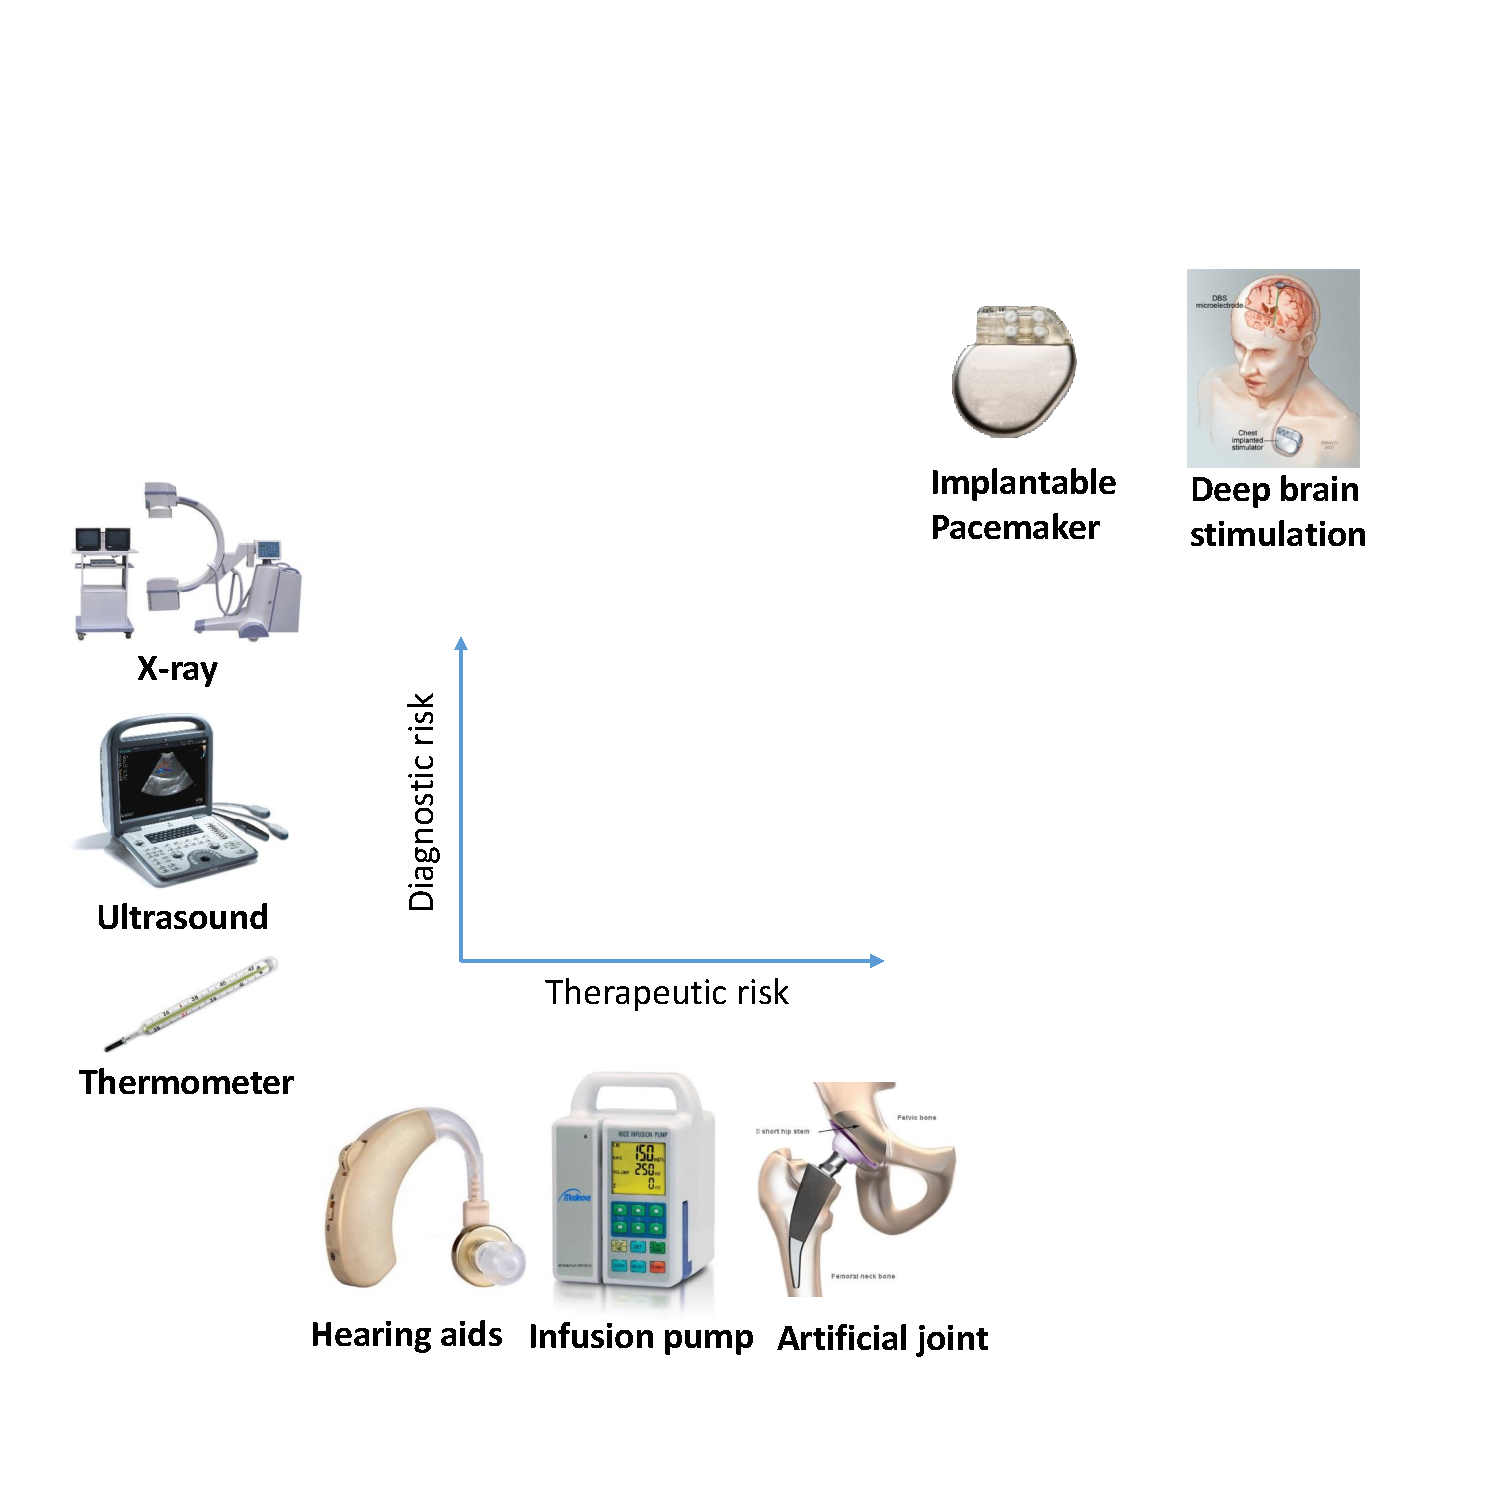
\includegraphics[width=\textwidth]{figs/devices_new.pdf}
		\caption{\small Figure of current medical devices}
		\label{fig:Cur}
\end{figure}


\section{Closing the Loop With the Patients}
Most medical devices operate with the patient in certain closed-loop manner. For diagnose-only devices, i.e. the X-ray machine, the physician operates the device to obtain patient data, perform diagnosis and deliver proper therapy to the patient (\figref{closed-loop}.(a)). For therapy-only devices, i.e. the infusion pumps, the physician operates the device to perform therapy on the patient according to previous diagnosis (\figref{closed-loop}.(b)). We denote these devices as \textbf{Open-loop Medical Devices} as there is no direct closed-loop interaction between the device and the patient. For open-loop devices, the safety of the patients is mostly guaranteed by the professionally-trained physicians in the loop. Device safety focus on providing accurate information to the physicians and faithfully operate as instructed by the physicians.

Among all the medical devices, there are devices with both diagnostic and therapeutic functions, i.e. implantable cardiac devices to treat cardiac arrhythmia, deep brain stimulation devices (\cite{Brain_sti}) to treat Parkinson's disease and artificial pancreas to treat Type 1 diabetes\footnote{The artificial pancreas is till under development by \cite{}}. These devices diagnose physiological conditions of the patient using sensory data, and deliver therapy accordingly (\figref{closed-loop}.(c)). These devices usually operate (semi-) autonomously with very little human intervention, thus malfunctions or inappropriate therapies from these devices cannot be corrected timely, which can cause serious adverse effects on patients' health. Therefore these devices are usually classified into the highest risk category and undergo the most stringent regulation. We denote them as \textbf{Closed-loop Medical Devices}. 
\begin{figure}[t]
		\centering
		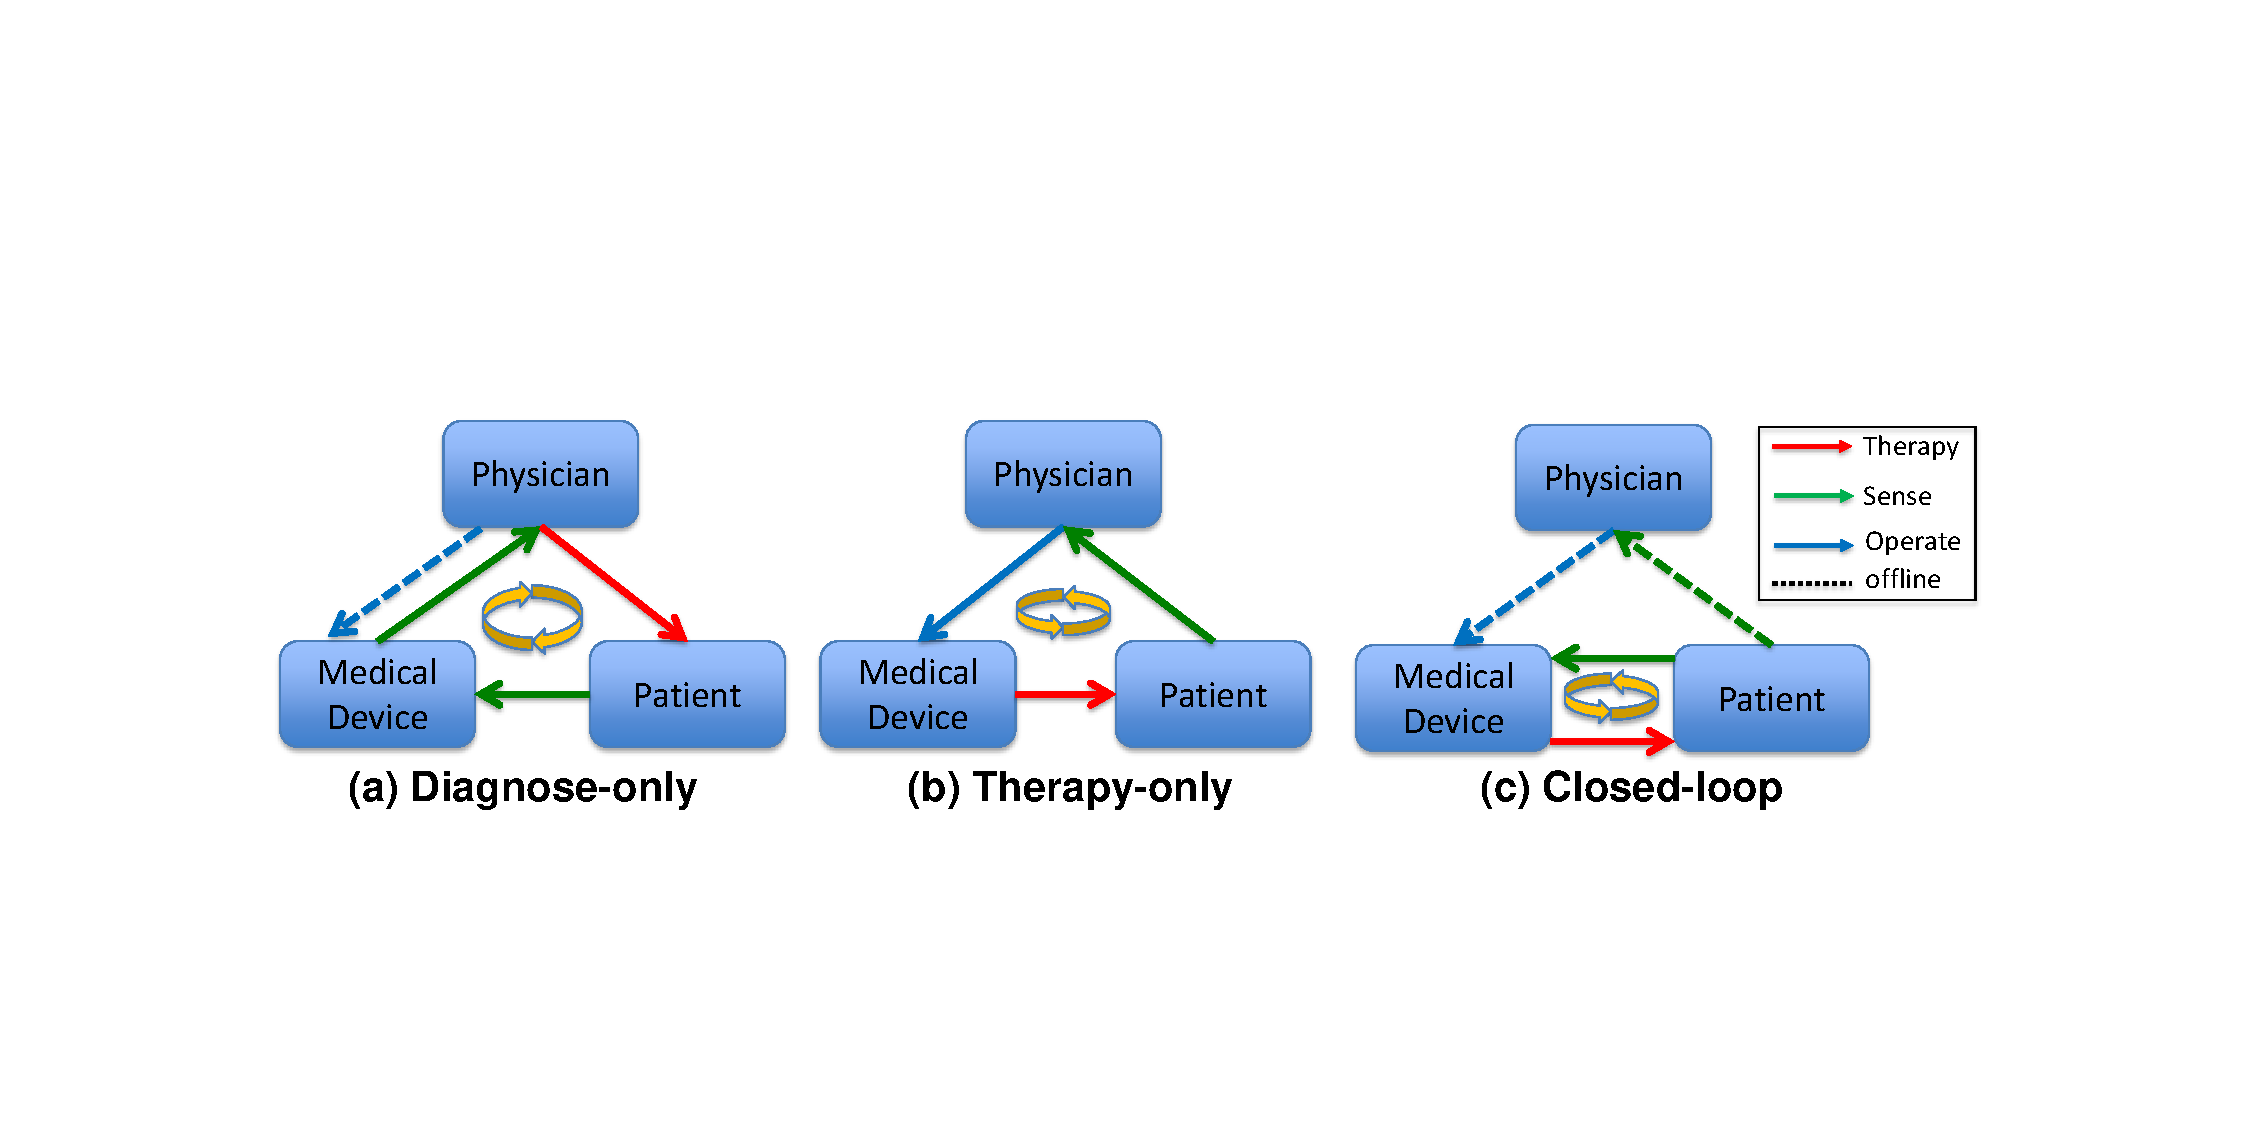
\includegraphics[width=\textwidth]{figs/closed-loop.pdf}
		\caption{\small Closing the Loop With the Patient}
		\label{fig:closed-loop}
\end{figure}
There are multiple challenges to develop safe and effective closed-loop medical devices:

\textbf{Closed-loop Interactions With Complex Physiology}\\
When using open-loop medical devices, the diagnosis and therapy decisions are made by medical professionals, who has abundant knowledge of human physiology. Therefore they are able to identify adverse health conditions and adjust the therapy accordingly. On the other hand, closed-loop medical devices have to make both the diagnosis and therapy decisions on their own. The domain expertise required to make those decisions has to be programmed into the device. It is impossible to encode all the knowledge of human physiology into the device. Therefore when conditions happen and are not programmed into the device, the device may deliver inappropriate therapy which can cause adverse effect on patient's health. 

With the development of new technology, new therapies to certain disease may arise and adopted by closed-loop devices. Certain closed-loop interactions between the device and the human physiology may not be well-understood, even to the medical professionals. Combinations of well-understood behaviors may also be the source for inappropriate therapies. In chapter \ref{ELT} we will demonstrate an example in which well-understood behaviors trigger unidentified inappropriate therapy by implantable pacemakers.

\textbf{Limited Diagnostic and Therapeutic Functions}\\
One fundamental rationale behind closed-loop medical devices is to enable the patients to live their normal lives without the dependance of cumbersome medical devices and/or the supervision of physicians. In fact, a large number of closed-loop medical devices are implantable devices. As a result, the sensing and therapy capabilities of the devices are limited, in order to increase portability and reduce invasiveness. Limited sensing capabilities may cause inaccurate diagnosis and therefore inappropriate therapy, as multiple conditions can map to the same sensor inputs. Due to limited therapy capabilities, there exists sub-optimal physiological conditions that are untreatable. The device may even trigger the conditions into less optimal conditions. In chapter \ref{mode_switch} we will demonstrate an example in which an untreatable condition is deteriorated into worse condition due to device interactions.

\textbf{Heavy Reliance on Software Control}\\\todo{I think we should not just focus on software so I put all these stats here instead of in front}
Due to the complexity of the diagnostic and therapeutic functions of the closed-loop devices, these functions are mostly controlled by their software components. 
Software embedded in a medical device, unlike electrical and mechanical components, does not fail due to corrosion, fatigue or have statistical failures of subcomponents. Software failures are uniquely sourced in the design and development of the system. %Unlike other industries such as consumer electronics where product life cycles are measured in months, software engineering for medical devices often spans a decade and must prioritize safety and efficacy over time to market. 
\begin{figure}[t]
		\centering
		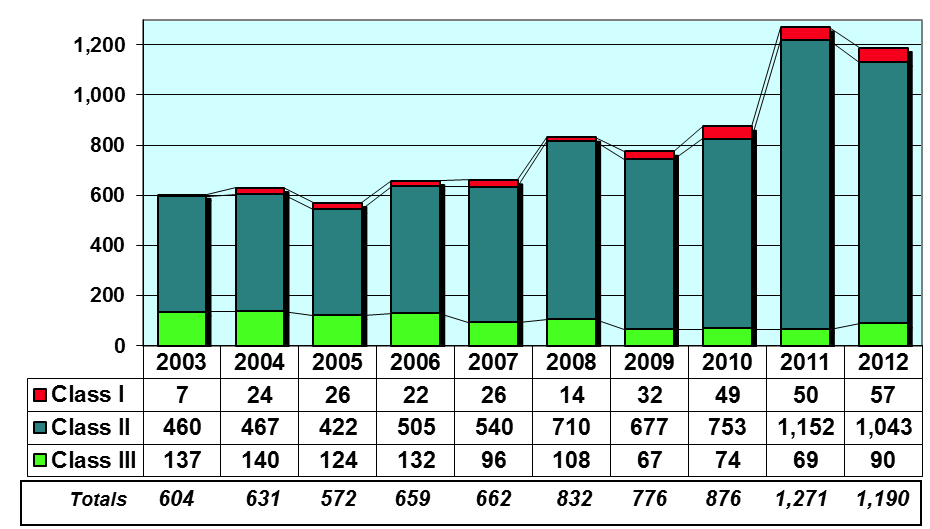
\includegraphics[width=0.8\textwidth]{figs/recalls.jpg}
		\caption{\small Figure of current medical devices}
		\label{fig:recalls}
\end{figure}
\begin{figure}[t]
		\centering
		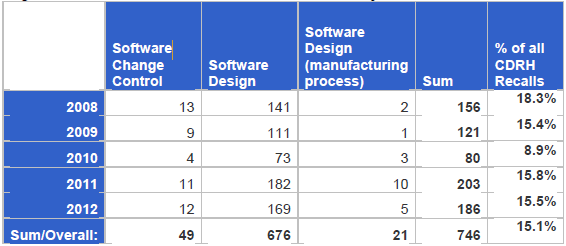
\includegraphics[width=0.8\textwidth]{figs/soft_recalls.jpg}
		\caption{\small Figure of current medical devices}
		\label{fig:soft_recalls}
\end{figure}
%  Over the course of the past four decades, cardiac rhythm management devices such as pacemakers and implantable cardioverter defibrillators (ICD) have grown in complexity and now have more than 80,000 to 100,000 lines of code (\cite{pauljones}). 
According to the US Food and Drug Administration, in 1996, 10\% of all medical device recalls were caused by software-related issues (\cite{medstats}). This percentage rose to an average of 15\% of recalls from 2008 to 2012 (\figref{soft_recalls}). Malfunctions of closed-loop medical devices usually have severe consequences, which will be categorized as \emph{Class I}, meaning there is a ``reasonable probability that use of these products will cause serious adverse health consequences or death.'' (\cite{medstats2,pacemakerrecalls,killedbycode}). 
	
\section{Regulation Efforts to Ensure Medical Device Safety}
The medical device industry is a regulated one to ensure the safety of the patients. The United States Food and Drug Administration (FDA) is the primary regulatory authority responsible for assuring the safety, efficacy and security of patients using medical devices. Based on the rationale that 1) manufacturers know their devices better than the regulator, and 2) the variety of medical devices requires a variety of approaches, the device manufacturers are responsibility to demonstrate the safety and efficacy of the medical devices. Manufacturers are required to complete pre-market submission before the devices can be released to the market. The level of requirements for the submission is determined by the safety classification of the devices. A set of general guidelines are recommended by the FDA (\cite{fda1, fda2, fda3}) which list the activities that need to be performed to ensure device safety. 

In safety-critical industries such as automotive electronics, avionics and nuclear systems, international standards are enforced for system development, evaluation, manufacturing and post-market changes (\cite{autosar,avsi}). This awareness is only beginning to enter the medical device industry as compliance with international standards are "recommended" in the aforementioned guidelines (\cite{formal_fda}). The basic rationale behind these standards is that: if all the risks/hazards of the device are identified and reasonably mitigated, and the device is developed with rigorous process, the device is reasonably safe. 

\figref{standards} demonstrates the fundamental standards to ensure medical device safety and their relationships. The IEC 60601 Medical Electrical Equipment - General requirements for basic safety and essential performance is a product safety standard that all electronic medical devices must comply to. There are emphasis on the safety of the software components. IEC 60324 specifies the processes and activities needed to perform during the software development life cycle to ensure software safety. 
Risk management is a core activity throughout the software development life cycle. ISO 14971 is specified for the application of risk management to medical devices. In addition, for each risk management activity of ISO 14971, ISO 80002-1 provides additional guidelines for the software component, which highlights and explains approaches to assuring that software safety is adequately addressed.
%The history of the FDA is a reactionary one, where each stage of evolution was in response to a major healthcare tragedy. 
\begin{figure}[t]
		\centering
		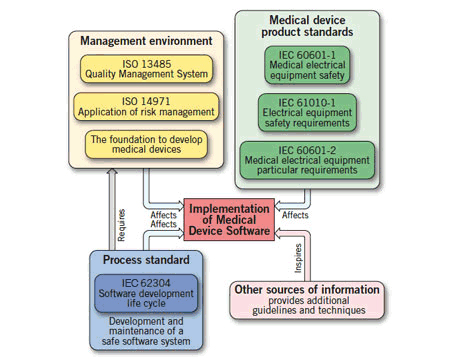
\includegraphics[width=0.8\textwidth]{figs/standards.pdf}
		\caption{\small International Standards Regarding Medical Device Safety}
		\label{fig:standards}
\end{figure}
\subsection{Risk Management}
Risk management includes risk analysis, risk evaluation and risk control. Fault Tree Analysis (FTA) is a common tool in risk analysis in which hazards of the system are first identified and the possible causes of the hazards are analyzed until the initial faults are reached. \figref{risks}.(a) demonstrate an example fault tree for automobile. The problem for fault tree analysis is that all possible causes are analyzed manually. In closed-loop medical devices, there may exist closed-loop interactions between the device and the patient that can cause certain hazard, but are unknown due to the limited physiological knowledge. \figref{risks}.(b) demonstrate a fault tree for a hazard of implantable pacemaker. There are several causes for undesirable fast ventricular rate. The well-understood cause is the intrinsic ventricular tachycardia (solid line). However, with pacemaker implanted, new mechanisms to cause hazard are introduced into the closed-loop system, as illustrated by the two branches with dotted lines. These two branches were not identified during the initial fault tree analysis, and were only identified after the devices have been released into the market, causing unnecessary adverse effects to the patients \cite{ELT}. Risks identified at this stage are also more costly to fix, increasing the cost for device development. \todo{Related to closed-loop model-checking}
\begin{figure}[t]
		\centering
		\includegraphics[width=\textwidth]{figs/fta_new.pdf}
		\caption{\small Fault Tree Analys (FTA) Examples. (a) FTA for a hazard for a car; (b) FTA for a hazard in implantable pacemaker}
		\label{fig:risks}
\end{figure}

After the fault tree has been constructed, probabilities for the initial faults are analyzed bottom up to calculate the probability of each hazard. The technique is called Failure Mode and Effects Analysis (FMEA). Then the risks are evaluated by assigning risk index to each hazard according to their occurrence and severity (\figref{risk_ana}). \todo{Related to requirement hierarchy}
\begin{figure}[t]
		\centering
		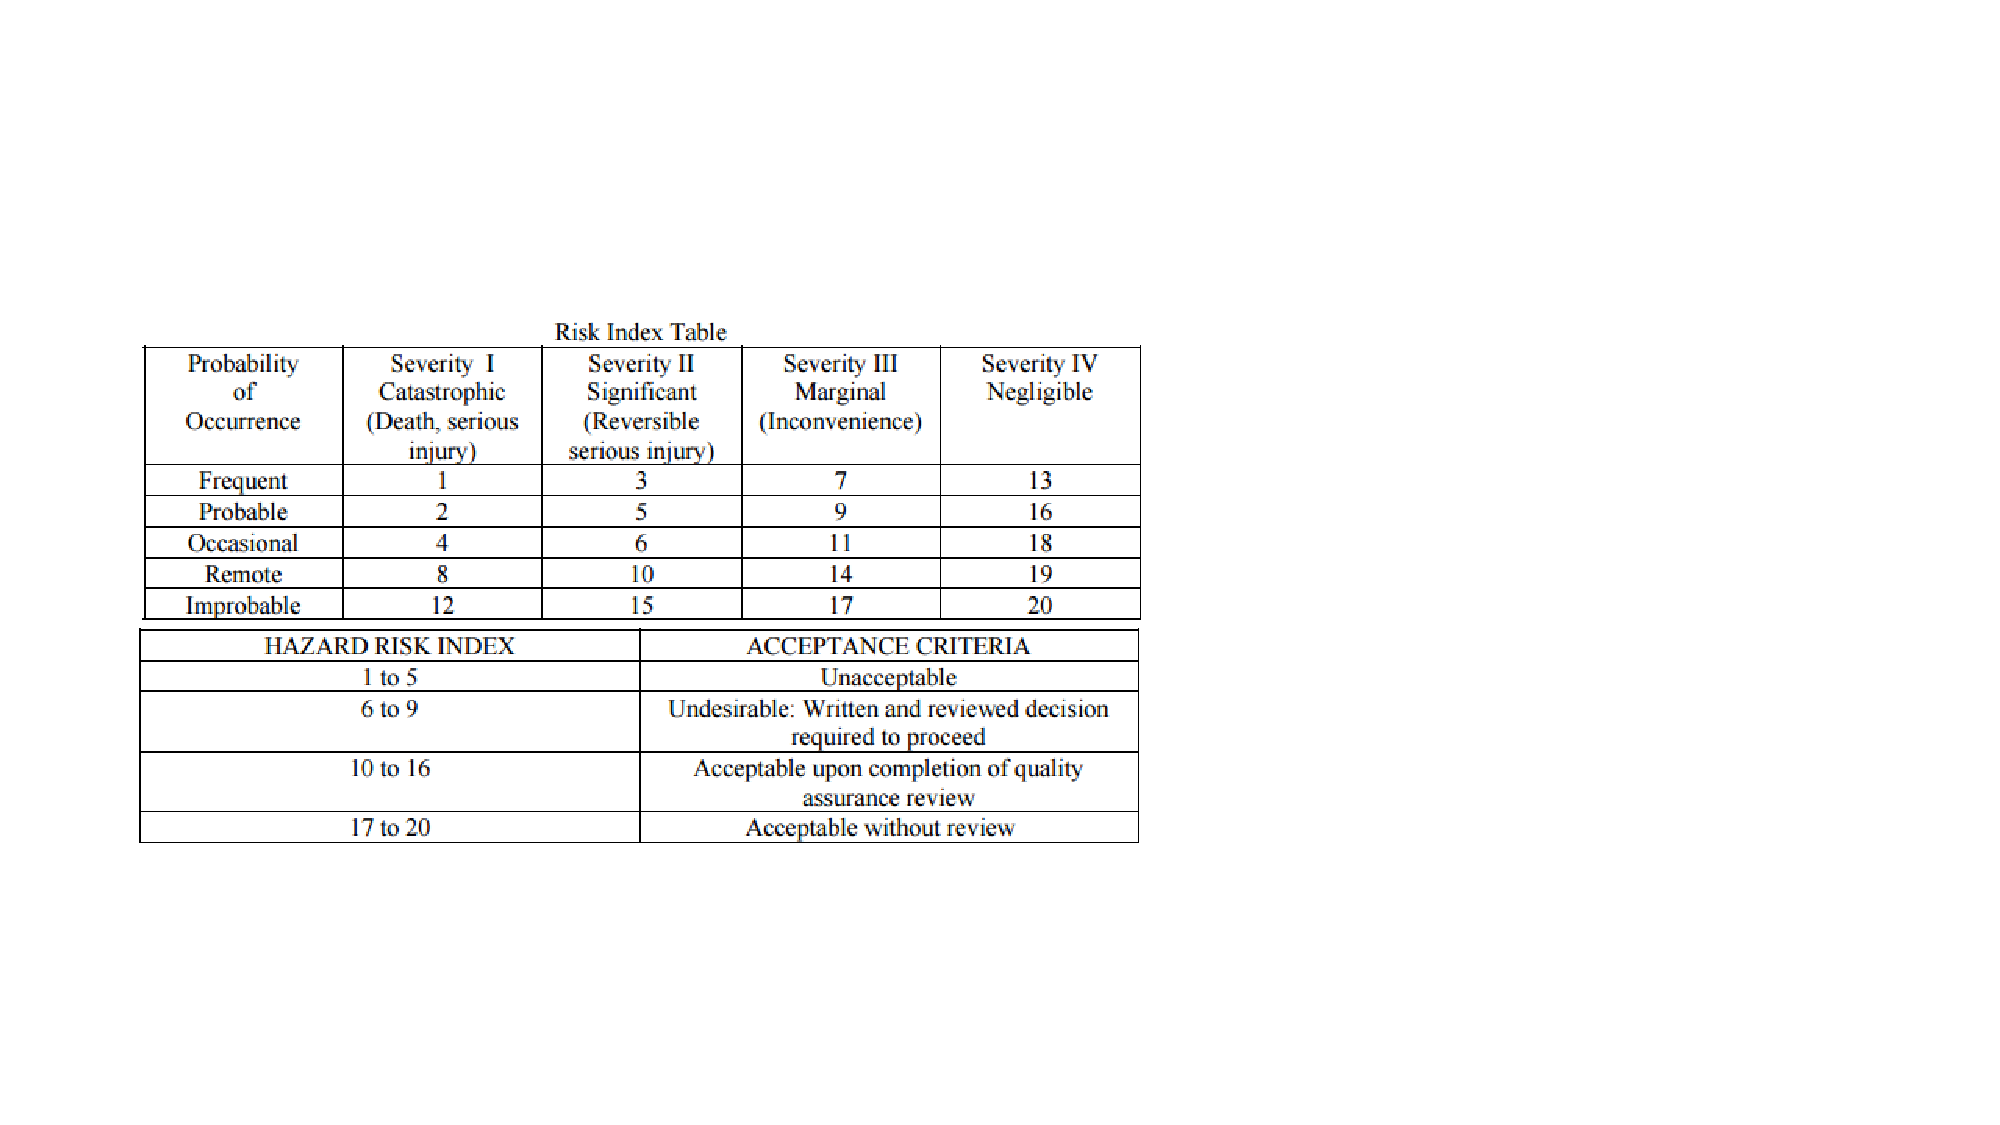
\includegraphics[width=\textwidth]{figs/risk_analysis.pdf}
		\caption{Top table: Risk index according to occurrence and severity. Bottom table: Risk control using risk index}
		\label{fig:risk_ana}
\end{figure}

After the risks are evaluated, different activities are required to mitigate the risks according to the risk index. After efforts made to reduce the risks, the risks should be re-evaluated to calculate the residual risk and analyze the risk/benefit. This is part of the risk control process.\todo{related to both the requirement hierarchy and model checking}
\subsection{Clinical Trials}
\todo{need some reference on this}Regardless of how rigorous the risk management and the device development process are, the devices have to be able to achieve their design goal on the real patient, which can only be evaluated in closed-loop with its physiological environment. Devices that have high risk factors, including the closed-loop medical devices, are required to submit clinical evidence for their safety and efficacy, often in form of clinical trials. In clinical trials the devices are used on carefully-selected population of patients following carefully-designed protocols, trying to obtain unambiguous results which can support the safety and/or efficacy of the devices. However, conducting clinical trials is very time consuming and expensive, and risks found during clinical trials are very expensive to fix. 
%Through the course of the 1980s, software began to play an increasing role in medical devices. Software, as it turns out, is one of those technologies not anticipated by prior regulation, and was waiting for its disaster to prompt regulatory action. It wasn't until the 1980s when a number of cancer patients received massive X-ray overdoses during radiation therapy with the Therac-25 linear accelerator. This lead to a number of investigations, perhaps the most thorough of which was that of \cite{therac}, which was rich with identified ways software could go wrong. Inadequate testing, dangerous code reuse, configuration management issues, inadequate manufacturer response, and failure to get to the root cause of the problem were among the leaders of the problems identified. The Therac-25 was an eye-opener for the FDA and legislators, and resulted in the Safe Medical Device Act of 1990. This finally required closer medical device tracking, post-market surveillance and recommendations on development, testing and validation of medical device software. \todo{Are these useful?}

%\subsection{Pre-market Submission Process}

%There are two processes through which a medical device can enter the market in U.S.: the Premarket Notification, also known as 510(k) \cite{510k}, and the Pre-Market Approval (PMA) \cite{PMA}. In a 510(k) submission the device manufacturers are only required to provide evidence that the device is \emph{substantial equivalent} to a \emph{predicate device}, which has been approved for the market. Therefore, the 510(k) submission does not directly require clinical evidence for the safety and effectiveness of the device, thus it is suitable for mostly low-risk devices like Class I and Class II devices.  The Pre-Market Approval (PMA) submission is a more stringent regulatory process in which direct clinical evidence is required to prove the safety and effectiveness of the device. However, not all Class III devices are subject to PMA submission. If a Class III device clears the 510(k) process and FDA has not requested PMA for that device, the device is still cleared for market release. A study shows that for Class III devices which PMA has been requested, the levels of evidence varies. Only 40\% of the PMA submissions are supported by controlled clinical trials, which provide the most rigorous clinical evidence \cite{cert_prob}. The lack of quality evidence is usually due to the high cost of the controlled clinical trials.

%\subsection{Safety and Efficacy Evidence}

%\todo[inline]{List of software standards}

%The FDA currently does not request or review the medical device software during pre-market submission. This is currently satisfied by the documentation of code inspections, static analysis, module-level testing and integration testing and their purpose is to establish ``reasonable assurance of safety and effectiveness''. These tests however fail to check for the correctness of the software and are largely open-loop tests that do not consider the context of the patient. Software is reviewed by the FDA only in the incident of a device recall. Software-related recalls are often issued in the form of \emph{Safety Alerts} by the %%%%%Food and Drug Administration (FDA) 
%FDA such as ``Safety alert - Pacemaker may revert to VVI mode at 70 beats/min if programmed to one of several specific ventricular pulse widths" (\cite{medstats}).


%\section{Challenges to Develop Safe Medical Device Software}
%\subsection{Safe Development Process vs. Safe Product}
%Conformance to the safety standards provides strong confidence on a safe development process. The belief is that a well-planned, systematic engineering process produces more reliable devices, especially if software is a component of the device (\cite{med-book}). However, there is no guarantee that safe process always yield safe devices. Recently there is growing interest on enforcing safety and efficacy evidence for the device itself. \cite{Wassyng} Due to the large variety of medical devices, there does not exist general safety and efficacy requirements that can be written into standard. As the result, evidence for product safety and efficacy varies in quality and organization. Assurance cases \cite{} have been proposed to help constructing safety arguments and organizing safety evidences. Assurance cases are currently "Recommanded" by FDA during regulation submission. (\cite{})


%\subsection{Multiple Stakeholders}
%For each medical device, there are 4 stakeholders: the regulator, the device manufacturer, the medical professional and the patient. All parties have the incentive to ensure the safety and efficacy of the device. With current regulation framework, the evidence for safety 
%\begin{figure}[t]
		%\centering
		%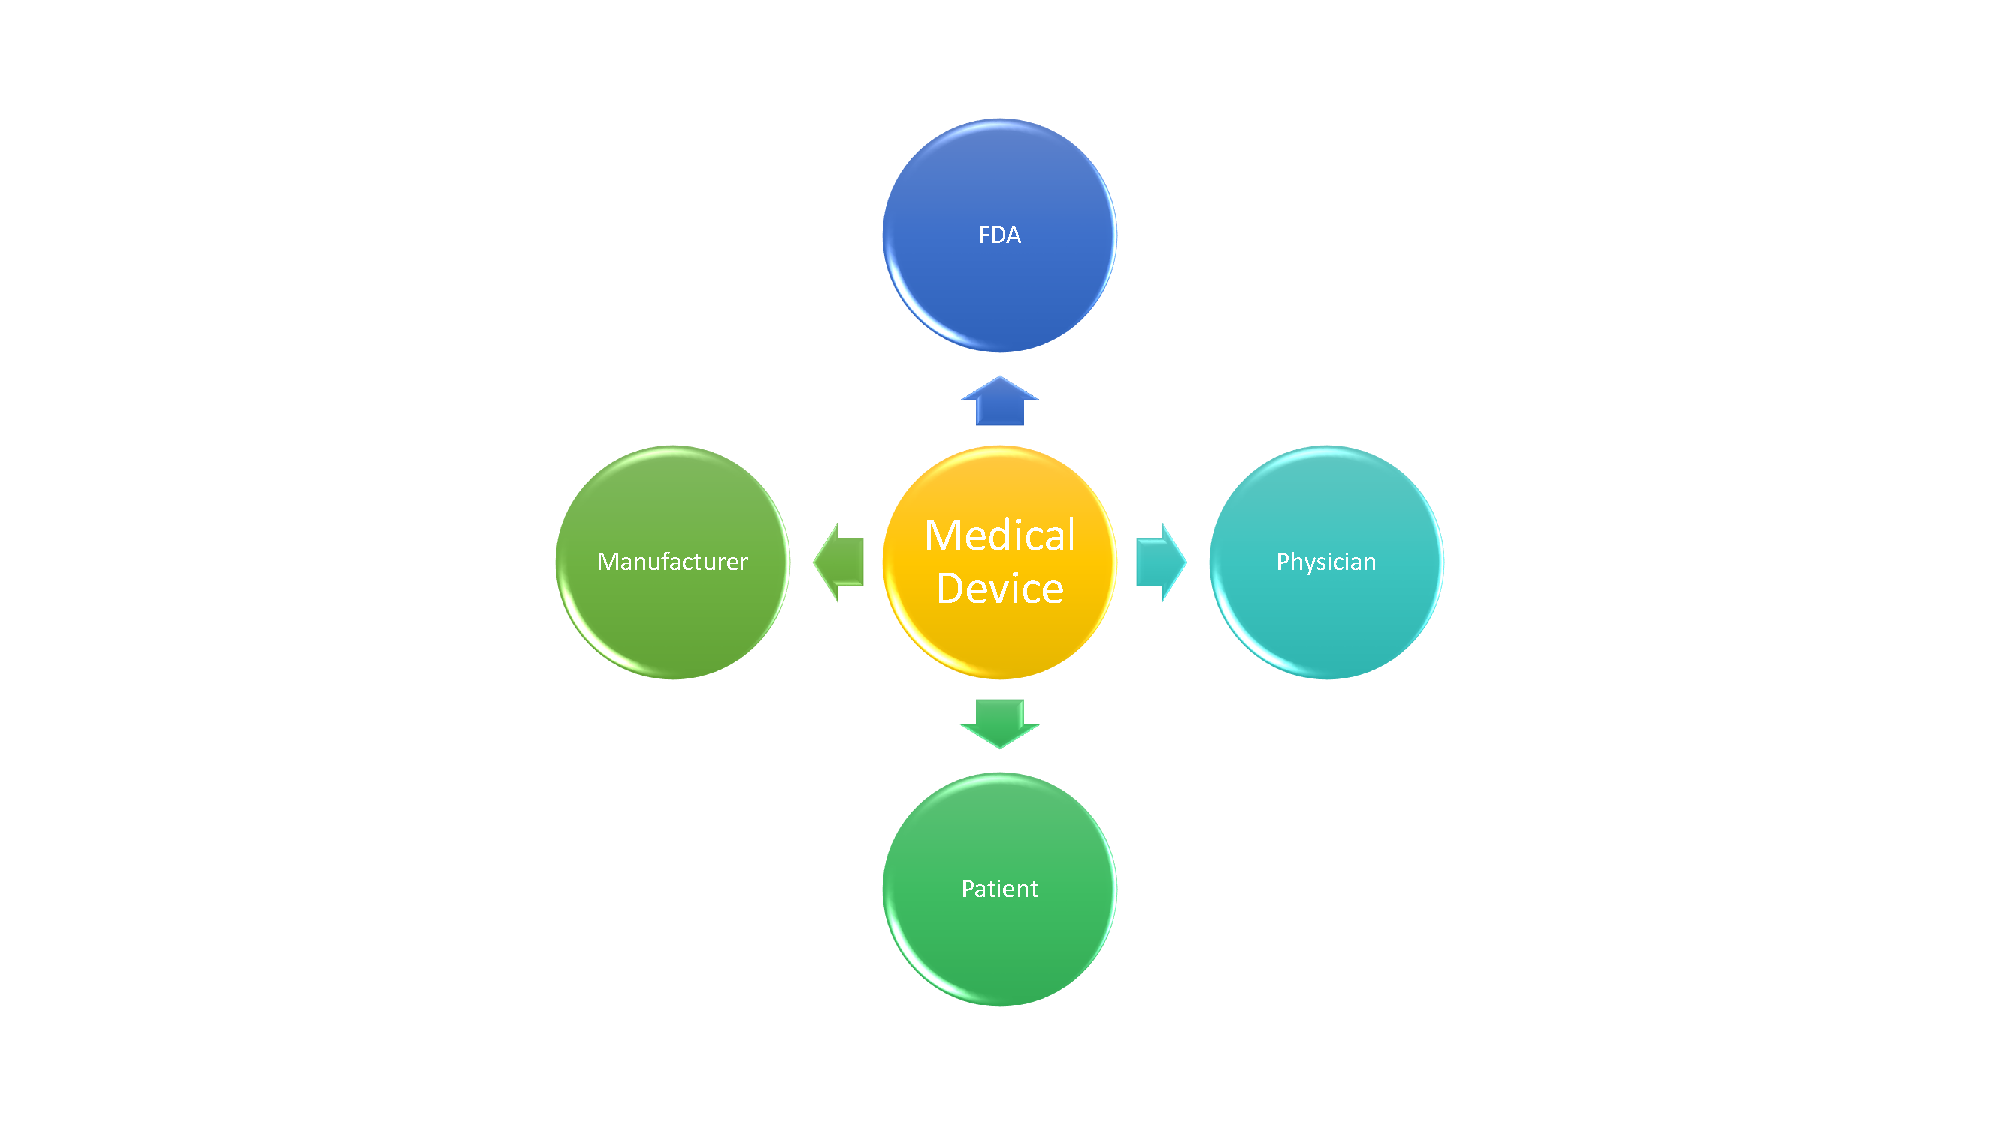
\includegraphics[width=0.8\textwidth]{figs/stakeholders.pdf}
		%\caption{\small Figure of current medical devices}
		%\label{fig:Cur}
%\end{figure}
%However, the medical domain presents its own unique set of challenges:\\
%\textbf{1. Closed-loop context:} Current evaluation of devices is open-loop and is unable to ensure the device never drives the patient into an unsafe state. Medical device testing and validation must thus be within the closed-loop context of the patient physiology. The context of the patient is a function of both the environment and the input from the device controller and must be captured by the device evaluation process.\\ 
%\textbf{2. Patient models:} There is a scarcity of patient models and clinically-relevant simulators for device design (\cite{pat-model}). High-fidelity models of interaction between the patient and device are needed to evaluate the safety and efficacy of device operation. Furthermore, these models must integrate the functional and formal aspects so that testing and verification are evaluated for the same patient states.\\
%\textbf{3. Adaptive patient-specific algorithms:} The therapy offered by the device must adapt to the environment and specific patient's condition. There is a need for validation algorithms to ensure that device control and optimization can cover large classes of patient conditions. 

%\section{The FDA and Medical Device Software}
%Before we delve into the current state of medical device software, it is useful to understand the evolution of the regulatory environment. 




%\section{Current Testing, Validation and Verification Approaches}
%In order to facilitate the early detection and correction of any software defects, the FDA has focused on infusion pumps due to the large number of recalls. In April 2010, the FDA began the ``Infusion Pump Improvement Initiative" which offers manufacturers ``the option of submitting the software code used in their infusion pumps for analysis by agency experts prior to premarket review of new or modified devices." 	\cite{}
%
%An effective software verification methodology is therefore needed for the risk analysis and certification of medical device software during the pre-market submission phase. While formal methods of verification are used for medical device software (\cite{challenge, challenge2, challenge3}), testing continues to be required because it can expose different kinds of problems (e.g. compiler bugs), can examine the program in its system context, and increases the diversity of evidence available. Testing for medical device software currently is ad hoc, error prone, and very expensive. Traditional methods of testing do not suffice as the test generation cannot be done independently of the current state of the patient and organ. The primary approach for system-level testing of medical devices is unit testing using a playback of pre-recorded electrogram and electrocardiogram signals (\cite{testing_imd, Vip}). This tests if the input signal triggers a particular response by the pacemaker, but has no means to evaluate if the response was appropriate for the patient condition. Furthermore, this approach of ``tape testing''\Hao{elaborate} is unable to check for safety violations due to inappropriate stimulus by the pacemaker. Pacemaker Mediated Tachycardia (PMT), a condition that is described later in this paper, is a strong example of why we need a model of the heart such as the one presented in this paper, which can be used for closed-loop system analysis. 
%PMT is a condition where the pacemaker inappropriately drives the heart-rate toward the upper rate limit. With a tape test, PMT would not occur and the response of the pacemaker could be classified as appropriate therapy.
%\begin{figure}[t]
		%\centering
		%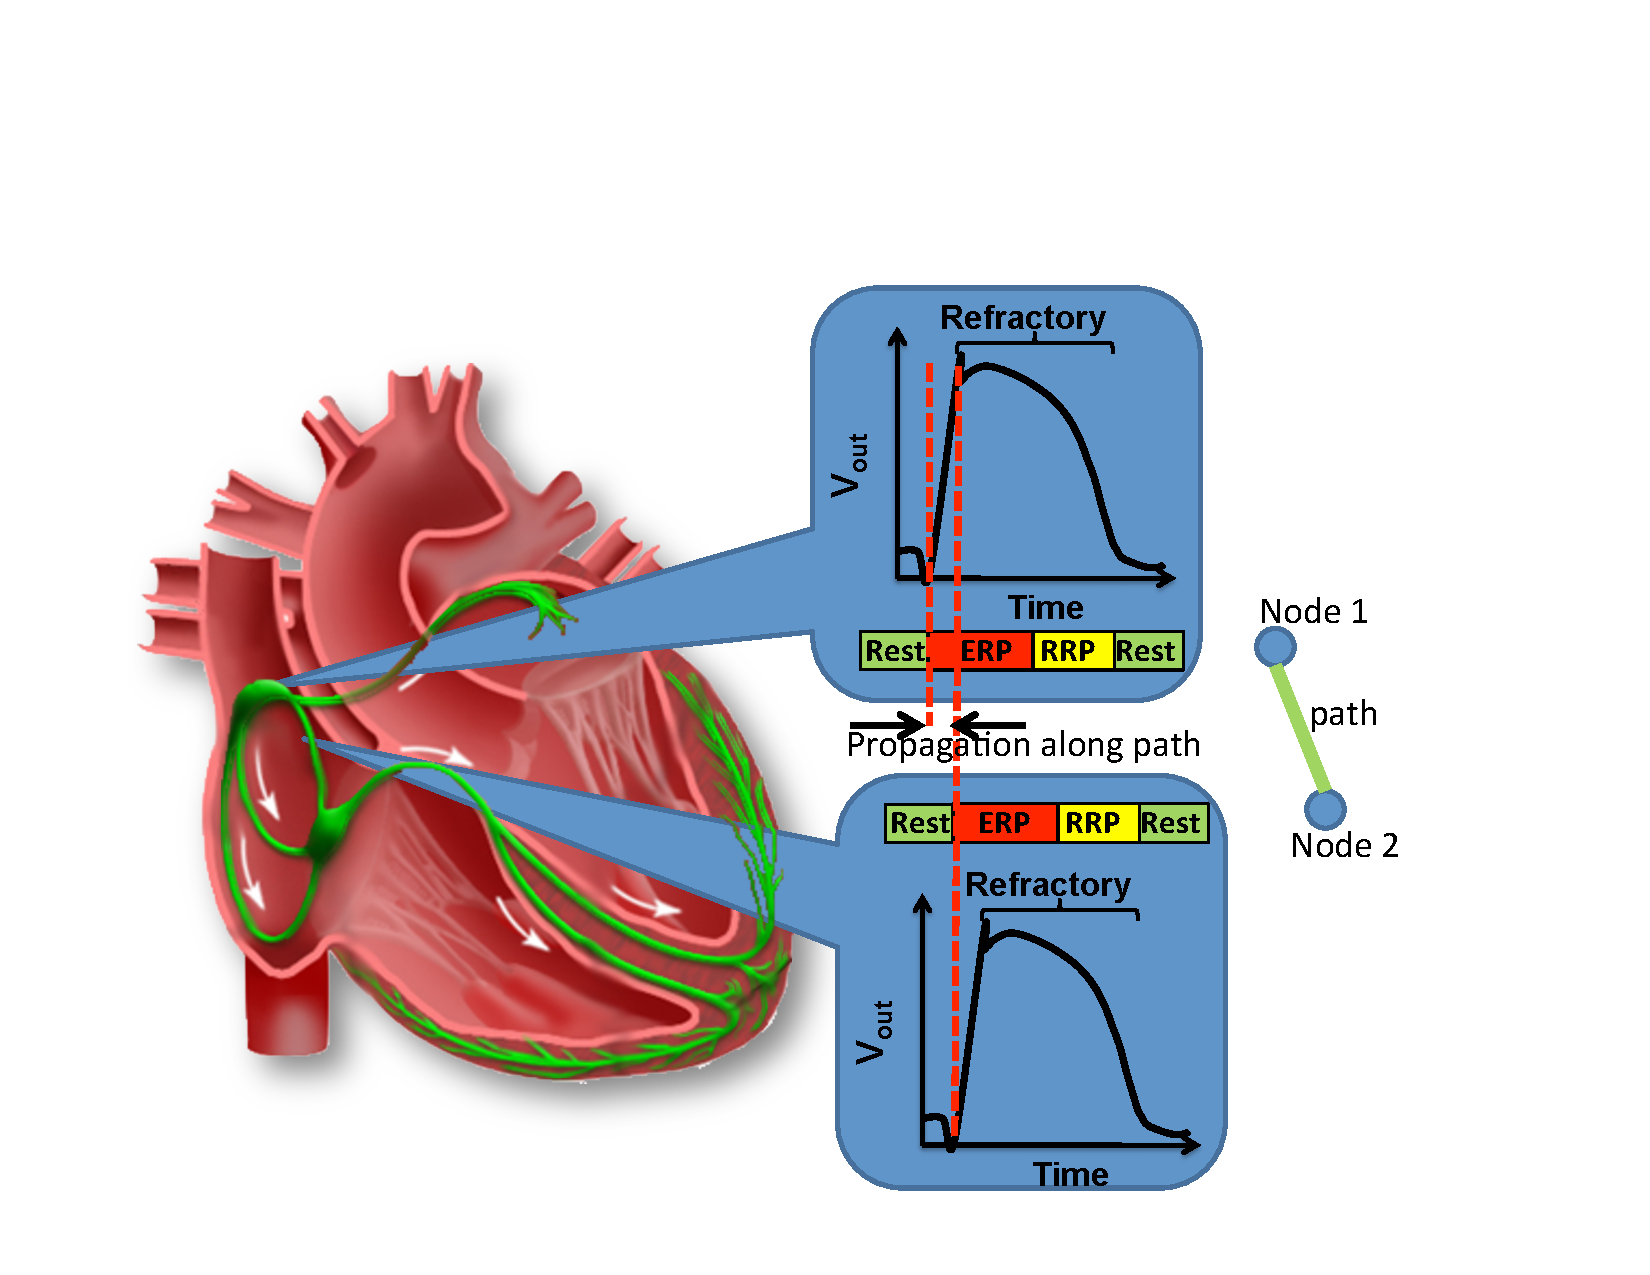
\includegraphics[width=0.8\textwidth]{figs/heartmodel.pdf}
		%%\vspace{-5pt}
		%\caption{\small By extracting timing and electric conduction information we model the signal activation, refractoriness and propagation across the heart tissue as a set of node and path automata.}
		  %%\vspace{-15pt}
		%\label{fig:heartmodel}
%\end{figure}
%As the testing environment (i.e., patient condition) is not entirely under the control of the tester, the problem changes significantly as a degree of nondeterminism is introduced in the process. Implantable medical devices are a primary example of Medical Cyber-Physical Systems where the safety and efficacy of the device and device software must be evaluated within a closed-loop context of the patient. The key challenge is in the generation of physiologically relevant tests such that the device does not provide inappropriate therapy, and does not adversely affect the safety of the patient. In addition, test generation must be interactive and adaptive such that the previous test stimulus affects the current state of the patient. The test generator must consider the current state when generating the next input in a way that advances the purpose of the test. The problem becomes one of the controller synthesis problems and cannot be addressed by an off-the-shelf model checker~\cite{rushby}.  
   %
%Formal methods have traditionally been used for verification of time-critical and safety-critical embedded systems \cite{form-meth}. Until recently, these methods have not been used for medical device certification. \cite{med-form3} presented the use of Extended Finite State Machines for model checking of a resuscitation device. Formal techniques have also been applied to improve medical device protocols (\cite{med-form2}) and safety (\cite{med-form1}), but the authors either used a simplified patient model or did not model the patient at all. 
\section{Improve Medical Device Safety with Model-based design}
Relying on clinical trials as the only closed-loop evaluation method to identify risks is not realistic. Model-based design has been proposed and applied in other industries like automobile (\cite{}), and can potentially help during the development process and provide extra confidence to the device before conducting clinical trials. However, unlike man-made systems like cars and aircrafts, physiological systems are less understood with larger variations. The lack of faithful models of physiological environment of the closed-loop medical devices is one of the reason that model-based design is not well-adopted in the medical device industry. 

With developments of computational tools and understanding of human physiology, computational models of human physiology have been developed which enable model-based closed-loop evaluations of the closed-loop medical devices. FDA is starting to recognize model simulation results as evidence for device safety and effectiveness. \cite{pancreas_paul} developed glucose-insulin models that can be used to evaluate control algorithms for artificial pancreas devices which can sense blood glucose and deliver insulin. Simulation results with the models have been recognized by FDA to replace animal trials, which significantly reduced cost (\cite{pancreas}).
\subsection{At Which Step Can We Help?}
Research results should fit in the framework in the real world.
Our work fits in the responsibilities of design validation teams in the device company.
Assume we have design artifacts like specifications (written form or model form), requirements, software or even physical devices

\section{Contributions}
In this paper we use implantable pacemaker as example to demonstrate how model-based design can help improve the safety and efficacy of the implantable pacemaker during software development. We demonstrate the development process from the perspective of the verification team of device manufacturers, therefore we assume to have full access to the pacemaker software design. The pacemaker software design is referenced from a dual chamber pacemaker from Boston Scientific (\cite{compass}).

Our proposed model-driven design (MDD) for closed-loop medical devices begins with developing heart models that can interact with real and modeled pacemakers (\cite{VHM_proc}). With the help of heart models, hazards themselves can be used as requirements directly and identify known and even unknown mechanisms that may trigger the hazards using techniques like model checking.

\todo{We may need to make another figure since this one does not show clearly how those activities fits in regulation}
As shown from the top of \figref{modeling_overview}, the heart-pacemaker closed-loop systems is first modeled abstractly to facilitate verification of the basic pacemaker design with maximum coverage (\cite{STTT13}). In our case, we use timed automata and the UPPAAL model checker at this design stage.

Next, the models are translated to more detailed models that take into account the complex dynamics of the heart and interaction with more detailed pacemaker model (\cite{vhm_ecrts10, vhm_embc11,vhm_iccps11}). We use Stateflow and Simulink at this design stage. These models are validated by physicians for their clinical relevance. The automatic model translation procedure, from UPPAAL to Stateflow, ensures that abstract models used for verification over-approximate the more detailed models used downstream (\cite{RTAS12}). Once the detailed models pass simulation-based testing with closed-loop dynamics, they are automatically generated into code and are subject to platform-level integration testing (\cite{vhm_website}). This MDD approach ensures the closed-loop safety properties are retained through the design toolchain and facilitates the development of verified software from verified models.
\begin{figure}[t]
		\centering
		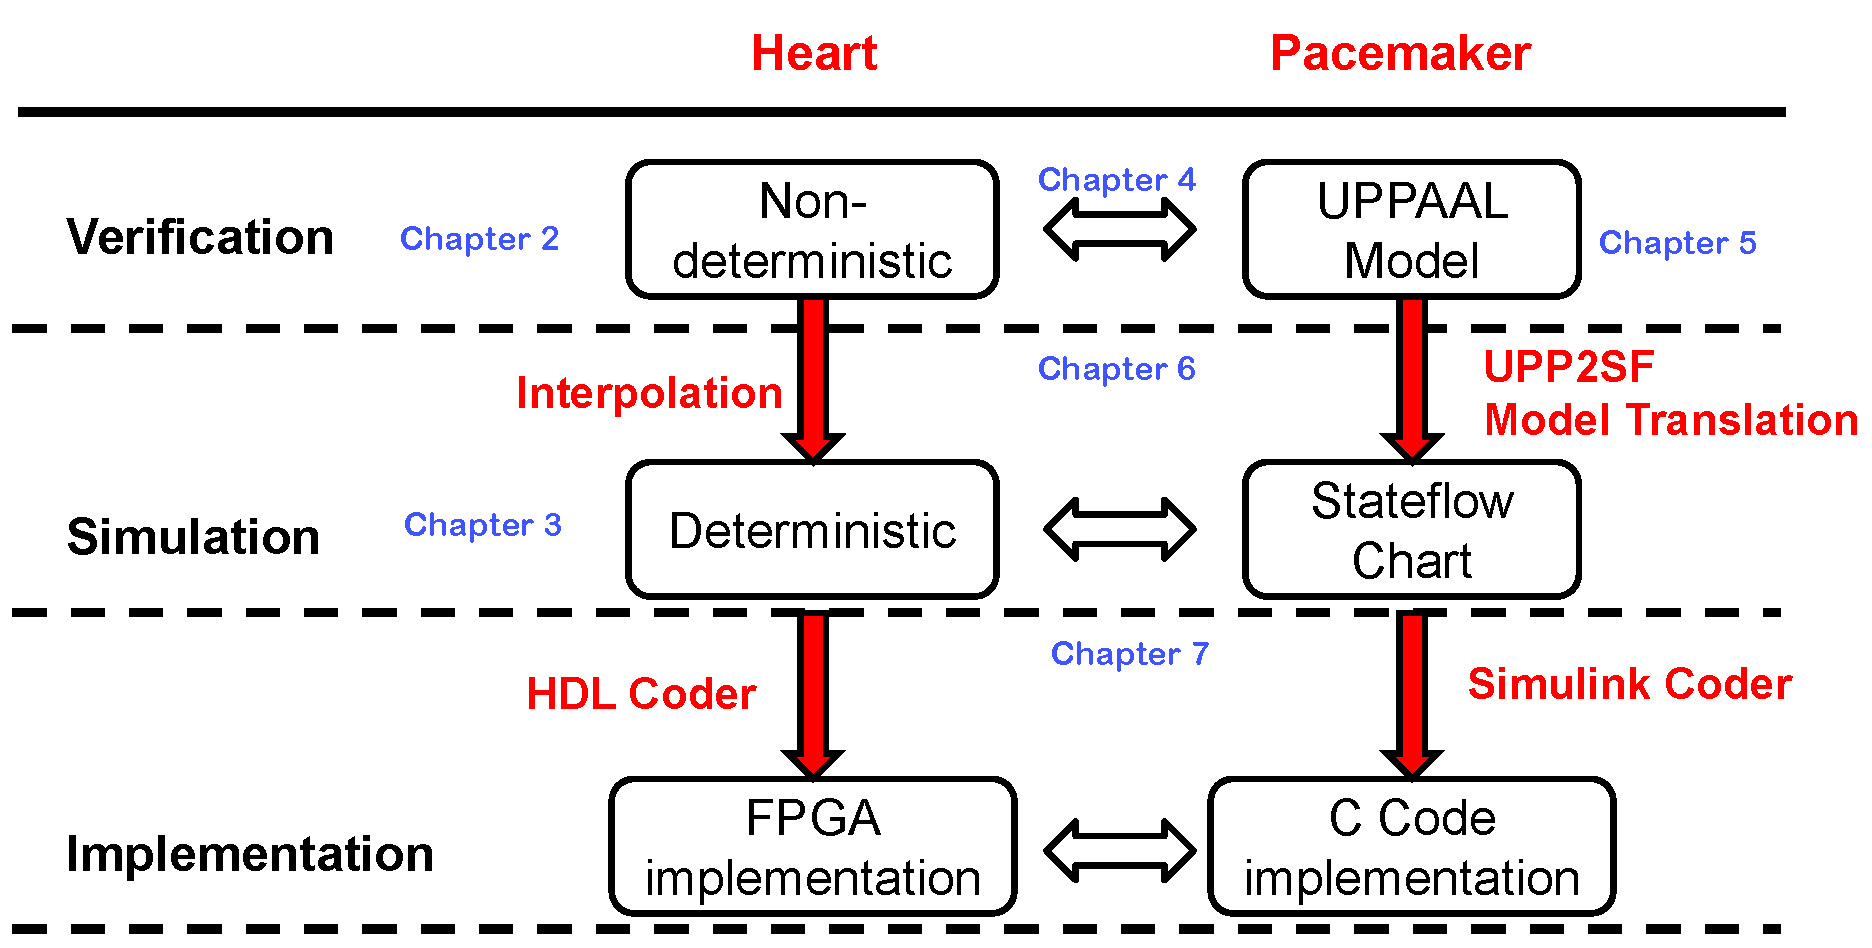
\includegraphics[width=0.8\textwidth]{figs/modeling_overview.jpg}
		%\vspace{-5pt}
		\caption{\small Model-driven design for verified models to verified code for the closed-loop heart and pacemaker system}
		  %\vspace{-15pt}
		\label{fig:modeling_overview}
\end{figure}

The focus of this effort is three-fold: (a) We developed an integrated functional (i.e., clinically-relevant) and formal (i.e., timed automata based) Virtual Heart Model  (VHM) (see \figref{heartmodel}) and a pacemaker device model for interactive and clinically relevant test generation.  (b) We provide a set of general and patient condition-specific pacemaker software requirements to ensure the safety of the patient is met under all cases, and (c) We provide a means to test and verify the closed-loop system over a variety of basic operation tests where the heart rate must be maintained, the atrial-ventricle synchrony must be enforced and complex closed-loop tests, where the pacemaker must not initiate tachycardia or perform improperly during lead displacement. With this approach of model-based testing, an executable functional model of the pacemaker is created at an early stage in the development process. This model-based methodology is an early step in addressing the urgent need for pre-market evaluation of medical device design and certification.


\section{Terminologies}
\todo{Should this come before or after the contribution section? it seems that the contributions have a good continuation from the problems}
Ensuring the safety of complex medical devices has drawn interest not only from stakeholders like regulators and industries, but also medical professionals and academia. Different communities have different interpretations over certain terminologies, causing misunderstandings. In this paper we adopt the terminologies from the regulation perspective, so that the results we have fit into the regulation framework. Most of the definitions are referred from the FDA guideline document General Principles of Software Validation (\cite{fda2}). Below are several terminologies that we use throughout the paper which worth clarifying.
\subsection{Requirements vs. Specifications}
By the definition of FDA (\cite{fda3}), the requirements of a system specify \textbf{what} the system should achieve and the specifications of a system specify \textbf{how} the system is designed to satisfy the requirements. For example, a requirement for an automobile is "Car should not hit objects". The corresponding specification can be "brake if the speed of the car is $x$ and the distance to the object is $y$". From the example we can see that a car satisfying its specification may not satisfy the requirement. In this paper, we use the word requirement in particular to denote the intended uses of the medical devices to improve physiological conditions.

\subsection{Validation vs. Verification vs. Testing}
As defined in \cite{fda2}, software validation is the confirmation by examination and provision of objective evidence that:
\begin{enumerate}
	\item software specifications conform to user needs and intended uses, and that
	\item the particular requirements implemented through software can be consistently fulfilled
\end{enumerate}
The first aspect ensures the device is safe and effective. The second aspect maintains the traceability of requirements throughout the development life cycle.
Software verification fulfills the second aspect of software validation by "providing objective evidence that the design outputs of a particular phase of the software development life cycle meet all of the specified requirements for that phase. "
\begin{figure}[t]
		\centering
		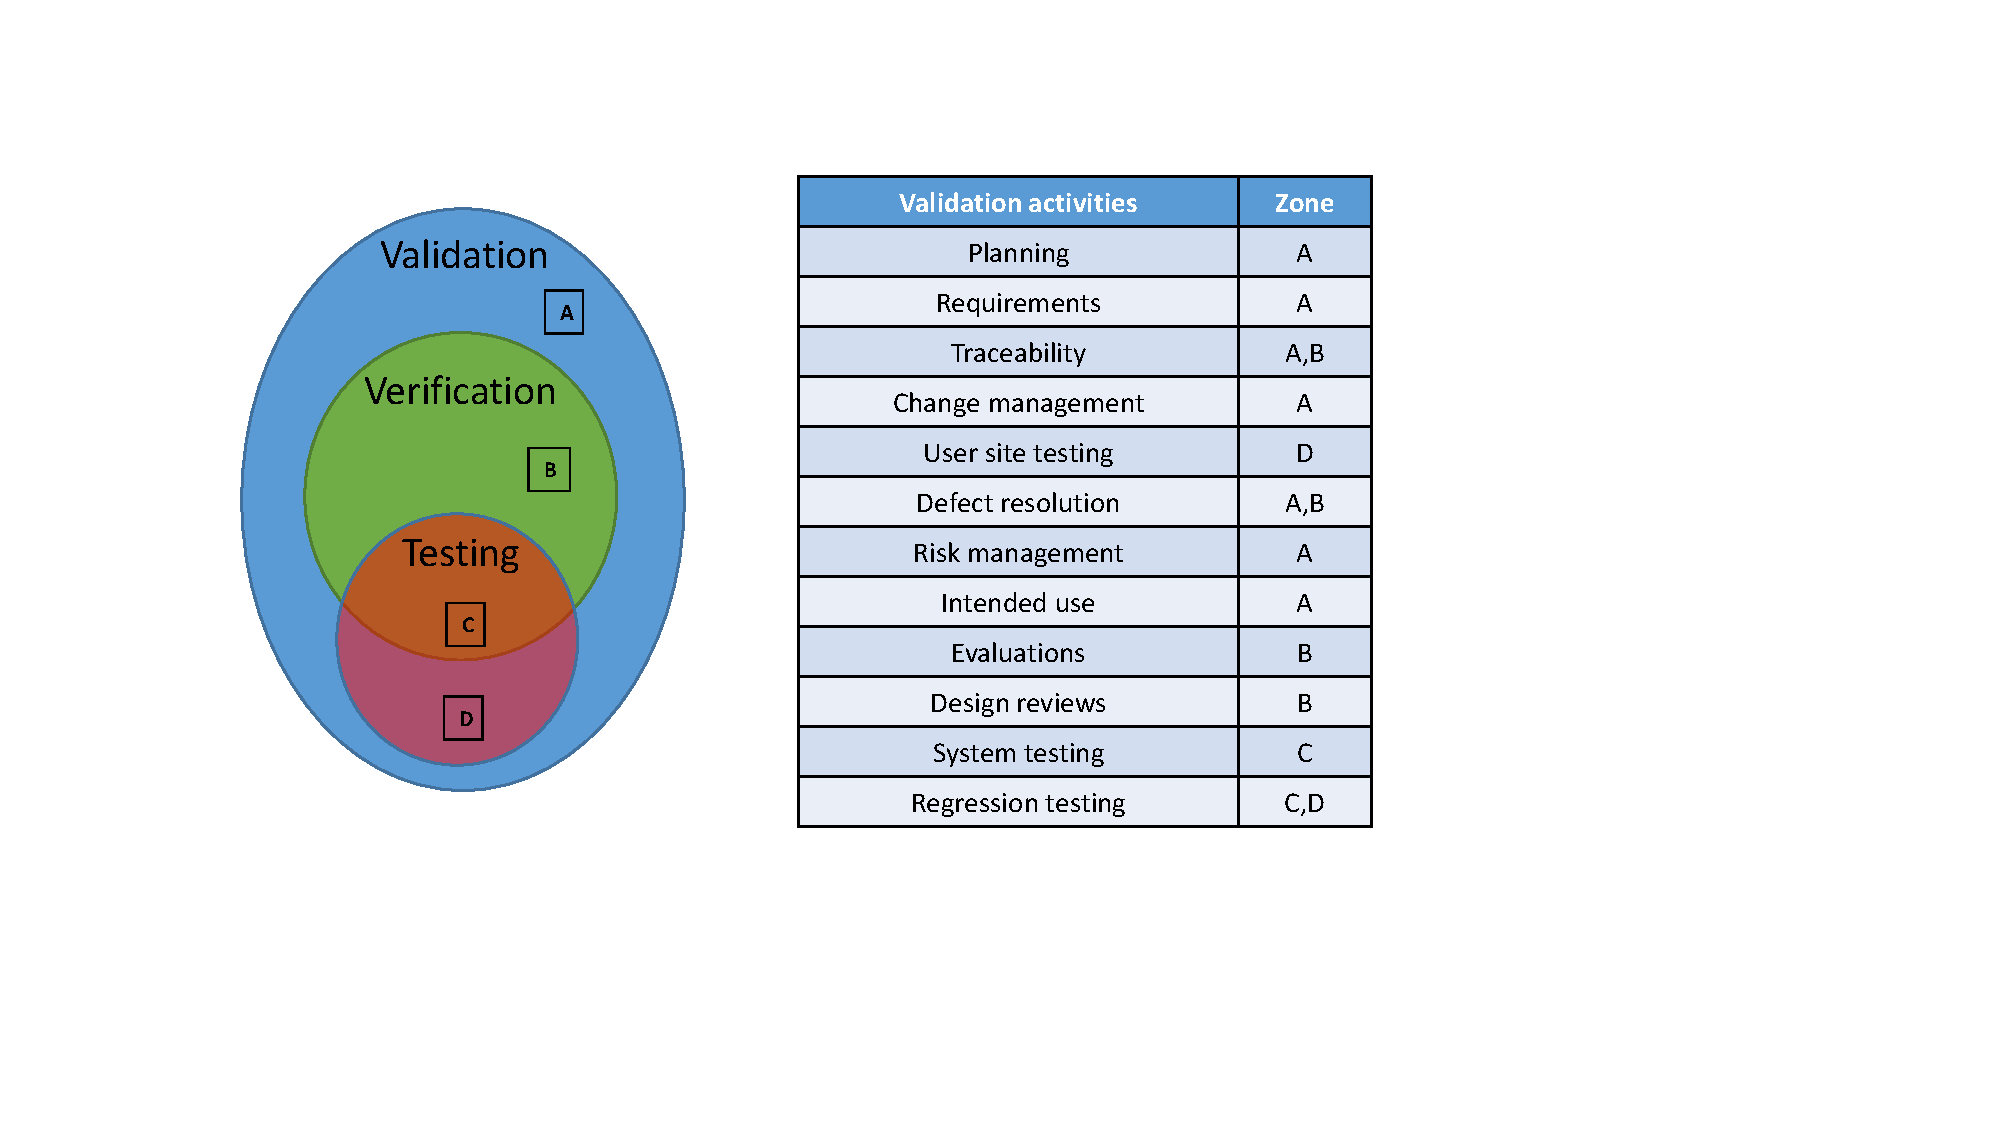
\includegraphics[width=\textwidth]{figs/validation.pdf}
		\caption{Validation activities during the software development life cycle (\cite{Vogel})}
		\label{fig:validation}
\end{figure}
Testing is the techniques that can be used for validation and/or verification. \figref{validation} illustrates the relationship between validation, verification and testing, and different activities during the software development life cycle to ensure the safety and effectiveness of the software.
\subsection{Closed-loop vs. Open-loop Evaluation}
In open-loop evaluation, i.e. open-loop testing, input sequences are send to the system and system outputs are compared with expected outputs. In open-loop testing, the system outputs do not affect the inputs afterward. In closed-loop evaluation, the environment of the system is taken into account. System outputs affect the state of the environment and thus affect the input sequences. For closed-loop medical devices, clinical trials are currently the most common closed-loop evaluation method. Enable closed-loop evaluation at model level requires models of the environment, which is human physiology for closed-loop medical devices.

Closed-loop evaluation does two things in model-based design 1) Enforce environmental constraints so that the test space is smaller and the test cases are physiological relevant. 2) Execution traces can be better interpreted as the physiological models encode domain knowledge. 
%%Through each of the chapters to follow, we cover different aspects of modeling the physiological system and the device, validating the models, running model checking on the closed-loop system and testing the deterministic systems derived from the abstract models. With the goal of 


\chapter{Understanding and Modeling the Physiological Environment}
\begin{itemize}
		\item How the device interacts with the environment?
		\item How much details should the environment models capture?
    \item What are the different modeling philosophies when developing environment models for different applications?
\end{itemize}

Medical devices are designed to interact with the human body aiming to improve physiological conditions of the patients. The knowledge of  the physiological context and how it can be changed by the devices is essential for 1) constructing physiological models; 2) understanding and encoding physiological requirements; 3) evaluating the closed-loop interactions between the human body and the devices. It is important to understand and model the physiological environment of the device at the level that 1) unnecessary details unrelated to the interaction between the device and the human are abstracted away, and 2) essential details required to differentiate different patient conditions are maintained.

Models (especially environment models) should be designed in accordance with their respective applications. During model-based development of medical devices, the environment model can be used for 1) closed-loop testing and 2) closed-loop model checking. Each application has different focus thus has very distinct requirements for the models. These requirements will affect the basic properties of the models, including 1) model complexity, 2) model identifiability etc. 

\textbf{Model Complexity} is generally measured in terms of the size of state space and/or computation complexity of state transitions, which affects the computation cost (memory and time) for closed-loop verification. The complexity requirements of an environment model is usually determined by 1) The complexity of the interactions between the environment model and the system model and 2) The complexity of the environment condition specified in the physiological requirements.

\textbf{Model Identifiability} is a metric of the feasibility/difficulty of identifying model parameters from data. It affects the validity of the model which is a key element for closed-loop verification. Model identifiability is generally affected by 1) Model complexity and 2) Data availability/quality. In general, the more complex the model structure is, the harder the model can be fully identified. There are two methods for model construction: non-parametric modeling in which no prior knowledge is assumed and the model construction is purely data-driven, and parametric modeling in which prior knowledge of the system is taken into account. For physiological modeling the data is generally scarce and there are abundant literature providing prior knowledge of the environment, it is more intuitive to use parametric modeling approaches.


In the following sections, we introduce the physiological context that the pacemaker operates in, and how to construct heart models for closed-loop verification of implantable pacemaker. Note that for two different applications the models are constructed differently as we address their respective requirements for environment models. 
\begin{figure}[!t]
\centering
		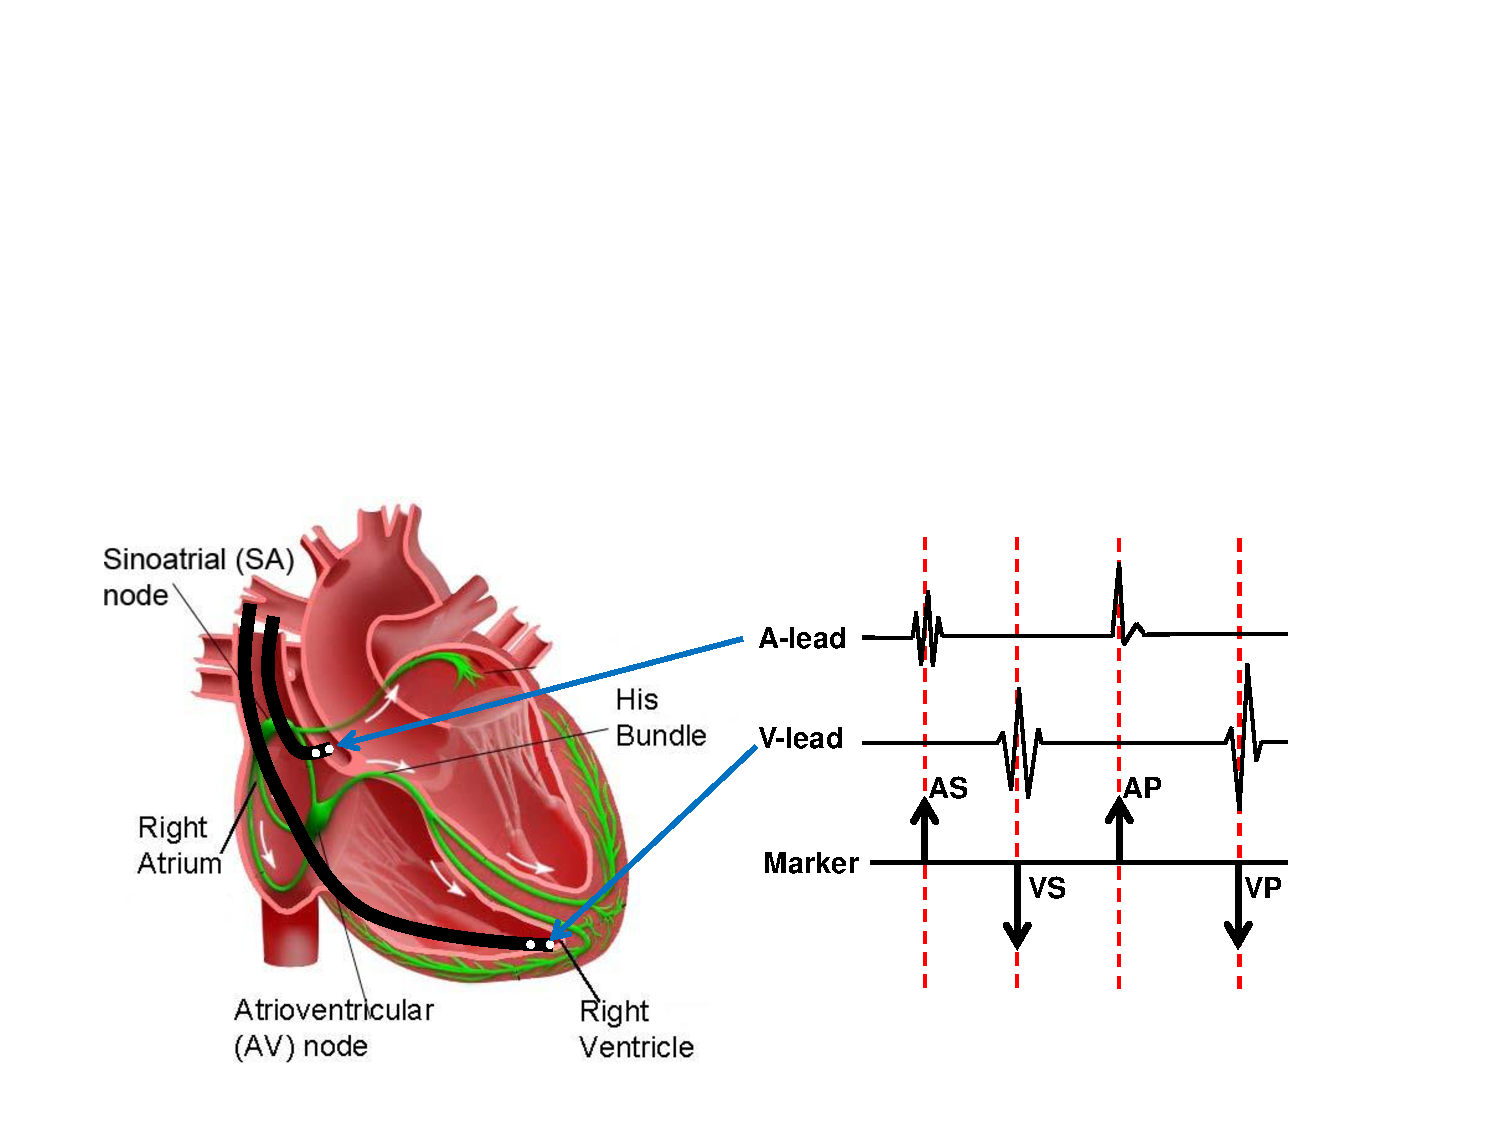
\includegraphics[width=0.9  \textwidth]{figs/egm.pdf}
		
%\vspace{-10pt}
\caption{\small }
\label{fig:probes}
%\vspace{-15pt}
\end{figure} 
\section{Physiological Context for Implantable Pacemaker}
The heart generates periodic electrical impulses to control heart rates according to physiological needs. These impulses conduct through the heart, triggering coordinated muscle contractions and pump blood to the rest of the body. The underlying pattern and timing of these impulses determine the heart's rhythm and are the key to proper heart functions. Derangements in this rhythm are referred to as \emph{arrhythmia}, which impair the heart's ability to pump blood and compromise the patients' health. Arrhythmia are categorized into so-called \textsf{Tachycardia} and \textsf{Bradycardia}. Tachycardia features undesirable fast heart rate which results in inefficient blood pumping. Bradycardia features slow heart rate which results in insufficient blood supply. Bradycardia are due to failure of impulse generation with anomalies in the SA node, or failure of impulse propagation where the conduction from atria to the ventricles is delayed or blocked. 

The electrical activities of the heart can be monitored and used to diagnose arrhythmia. The most well-known method is Electrocardiogram (ECG or EKG), which measure the integration of electrical activities of the heart measured along different axis on the body surface. The electrical activities can also be measured by inserting electrodes through the vein into the heart. The electrodes are placed against the inside heart wall and localized electrical activities can be measured. (\figref{probes}.a) Physicians can also deliver pacing sequence through the electrodes to explore the heart conditions. This procedure is referred to as Electrophysiological (EP) Testing  (\cite{josephson}) and the signals are referred to as electrograms (EGMs) (\figref{probes}.b). %The timing and morphology of the  ECG and EGM singnals can be used to diagnose arrhythmia.

%Implantable pacemakers follow the principle of EP testing. For a dual chamber pacemaker, two leads are inserted into the right atrium and right ventricle, respectively. The pacemaker senses the intrinsic generation and conduction of the electrical signals in the two chambers and deliver electrical pacing when the heart rate and/or atria-to-ventricles conduction interval are abnormal.
The implantable cardiac pacemakers are rhythm management devices designed to treat bradycardia. A typical dual chamber pacemaker has two leads inserted into the heart through the veins which can measure the local electrical activities of the right atrium and right ventricle, respectively. According to the timing between sensed impulses the pacemaker can deliver electrical pacing to the corresponding chamber to maintain proper heart rhythm.
\begin{figure}[!t]
\center
%\vspace{-10pt}
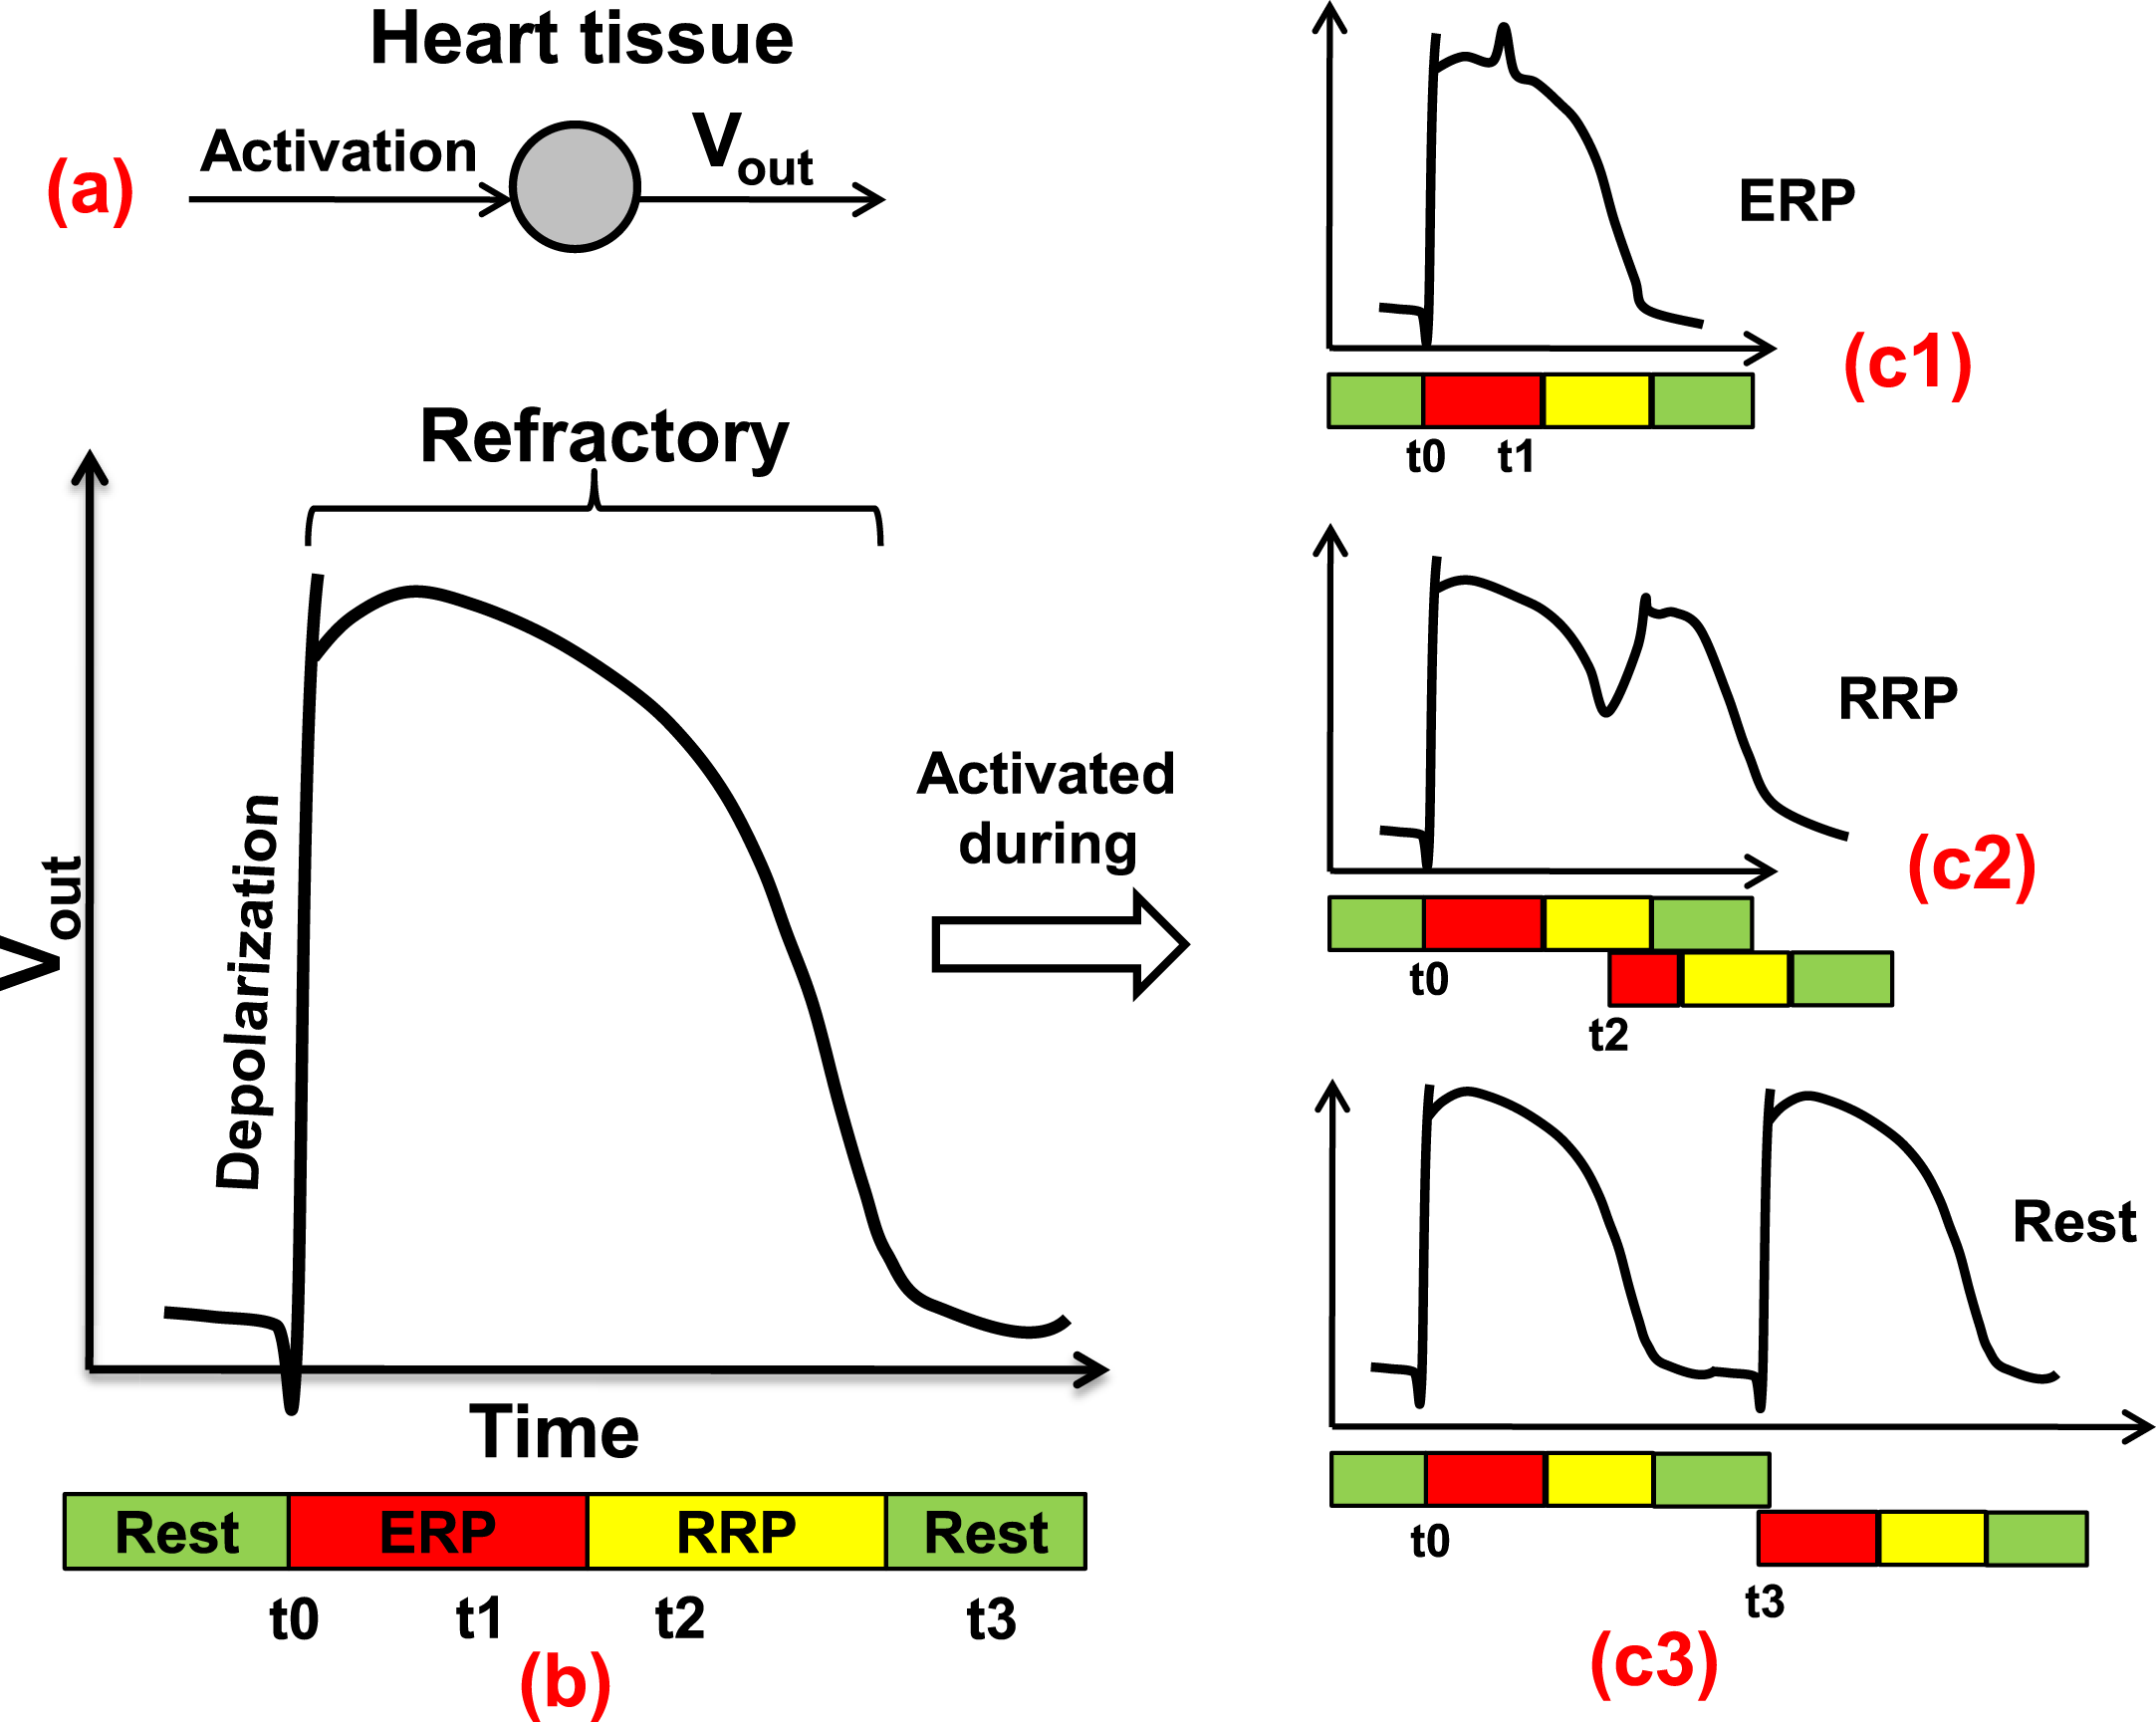
\includegraphics[width=0.7\textwidth]{figs/refractory.png}
%\vspace{-10pt}
\caption{(a) The generation of Action potential; (b) Action potential; (c1) The second activation arrived during ERP; (c2) Arrived during RRP; (c3) Arrived after refractory.}
\label{fig:refractory}
%\vspace{-10pt}
\end{figure} 
\subsection{Cellular Level ElectroPhysiology}
The contraction of heart muscles can be triggered by external voltage applied to the cell. After the activation, a transmembrane voltage change over time can be sensed due to ion channel activities, which is referred to as an Action Potential (\figref{refractory}(a)). The upstroke of the action potential is called depolarization, during which the muscle will contract. The voltage change caused by the depolarization will depolarize the cells nearby, which causes an activation wave across the heart. After the depolarization there is a refractory period during which the cell recovers to the pre-excitation state and the voltage drops down to the resting potential. The refractory period can be divided into \emph{Effective Refractory Period (ERP)} and \emph{Relative Refractory Period (RRP)} (\figref{refractory}(b)). During ERP, the cell cannot be depolarized due to the lack of the ion. As the result, the activation wave will be "blocked" at the tissue during ERP (\figref{refractory}(c1)). During RRP, the cell is partially recovered and the cell can be depolarized. However, the new action potential generated by the depolarization will have different morphology, thus affecting the refractory periods of the tissue and conduction delay of the activation wave (\figref{refractory}(c2)). \figref{refractory}(c1)-(c3) show the action potential shape change and corresponding timing change in refractory periods when the cell is activated at time stamp $t1$, $t2$, $t3$ after the initial activation $t0$. 



\subsection{Electrical conduction system of the heart}
Heart tissue with different timing parameters assemble the electrical conduction system to ensure coordinated contraction of the heart. First, specialized tissue at the Sinoatrial (SA) node periodically and spontaneously self-depolarizes. This is controlled by the nervous system and the SA node is the primary and natural pacemaker of the heart. The activation signal then travels through both atria, causing contraction and pushes blood into the ventricles. Then the activation is delayed at the Atrioventricular (AV) node which allows the ventricles to fill fully. The fast-conducting His-Purkinje system then spreads the activation signal within both the ventricles. The simultaneous contraction of the ventricle muscles will push the blood out of the heart.
%\begin{figure*}[!t]
%\centering
		%\subfigure [\small]{			
		%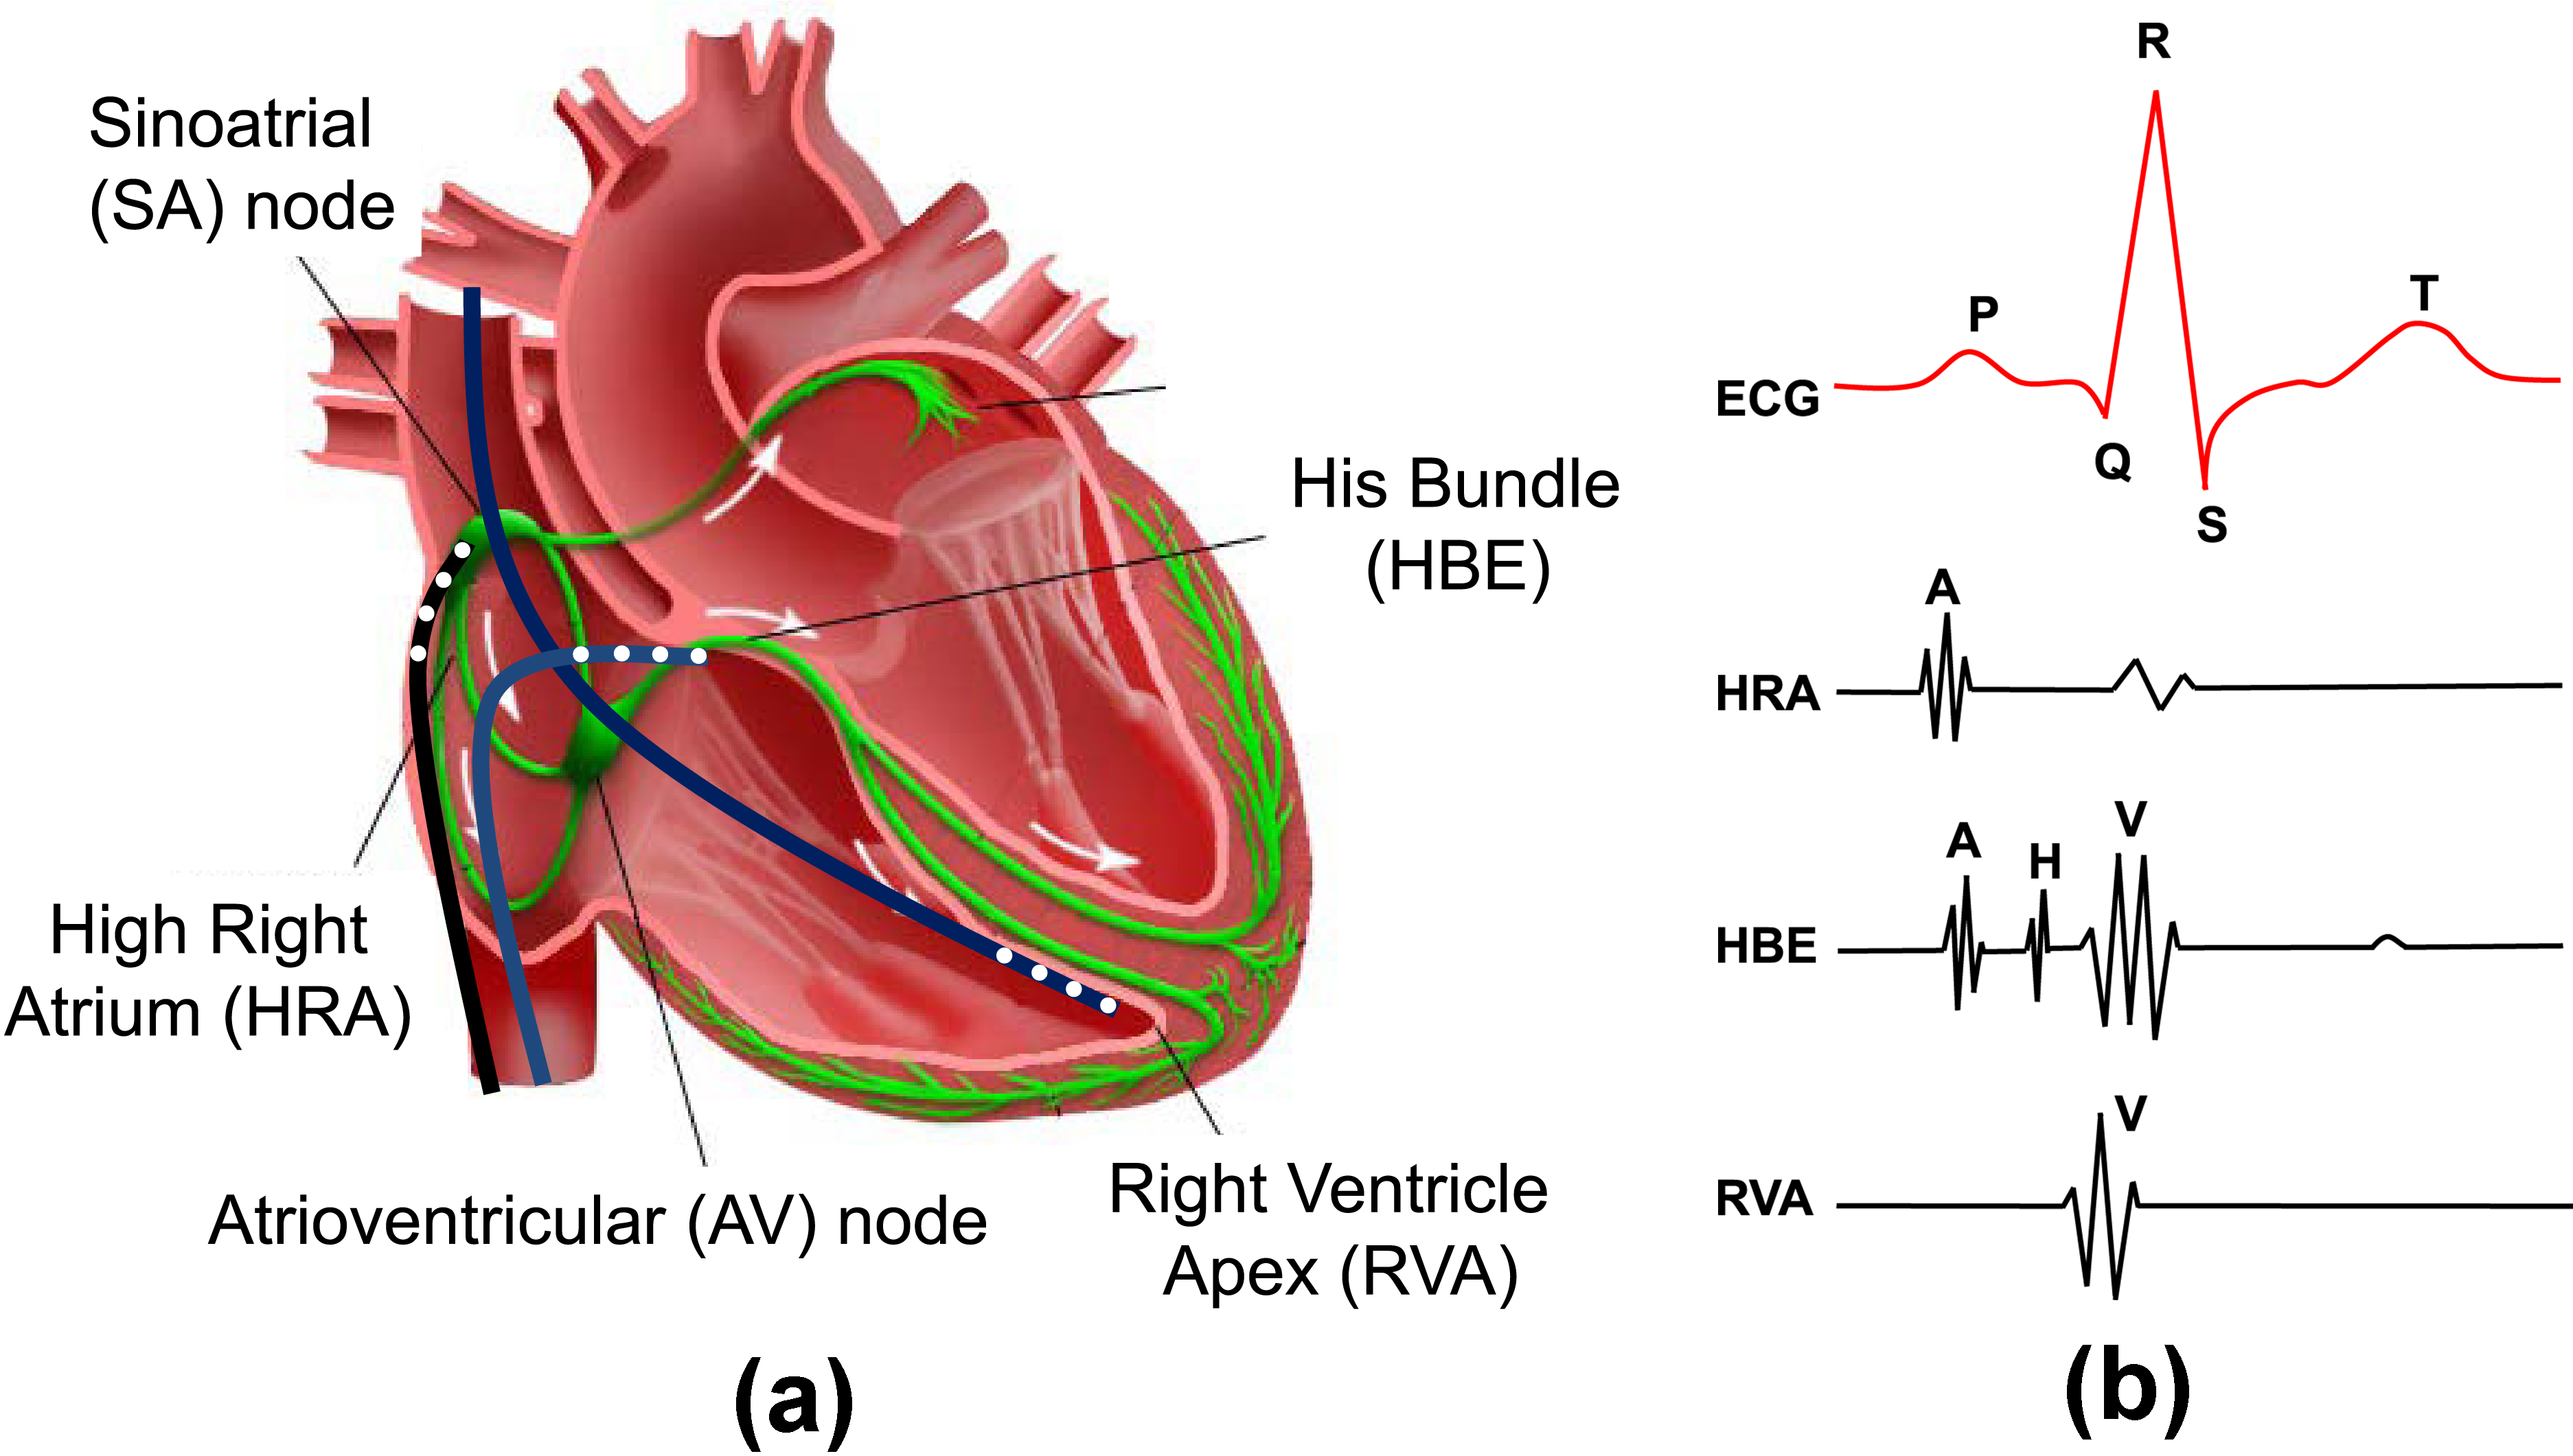
\includegraphics[width=0.3  \textwidth]{figs/probes.png}
		%\label{fig:probes}
		%} 
%
		%\subfigure [\small] 
		%{
		%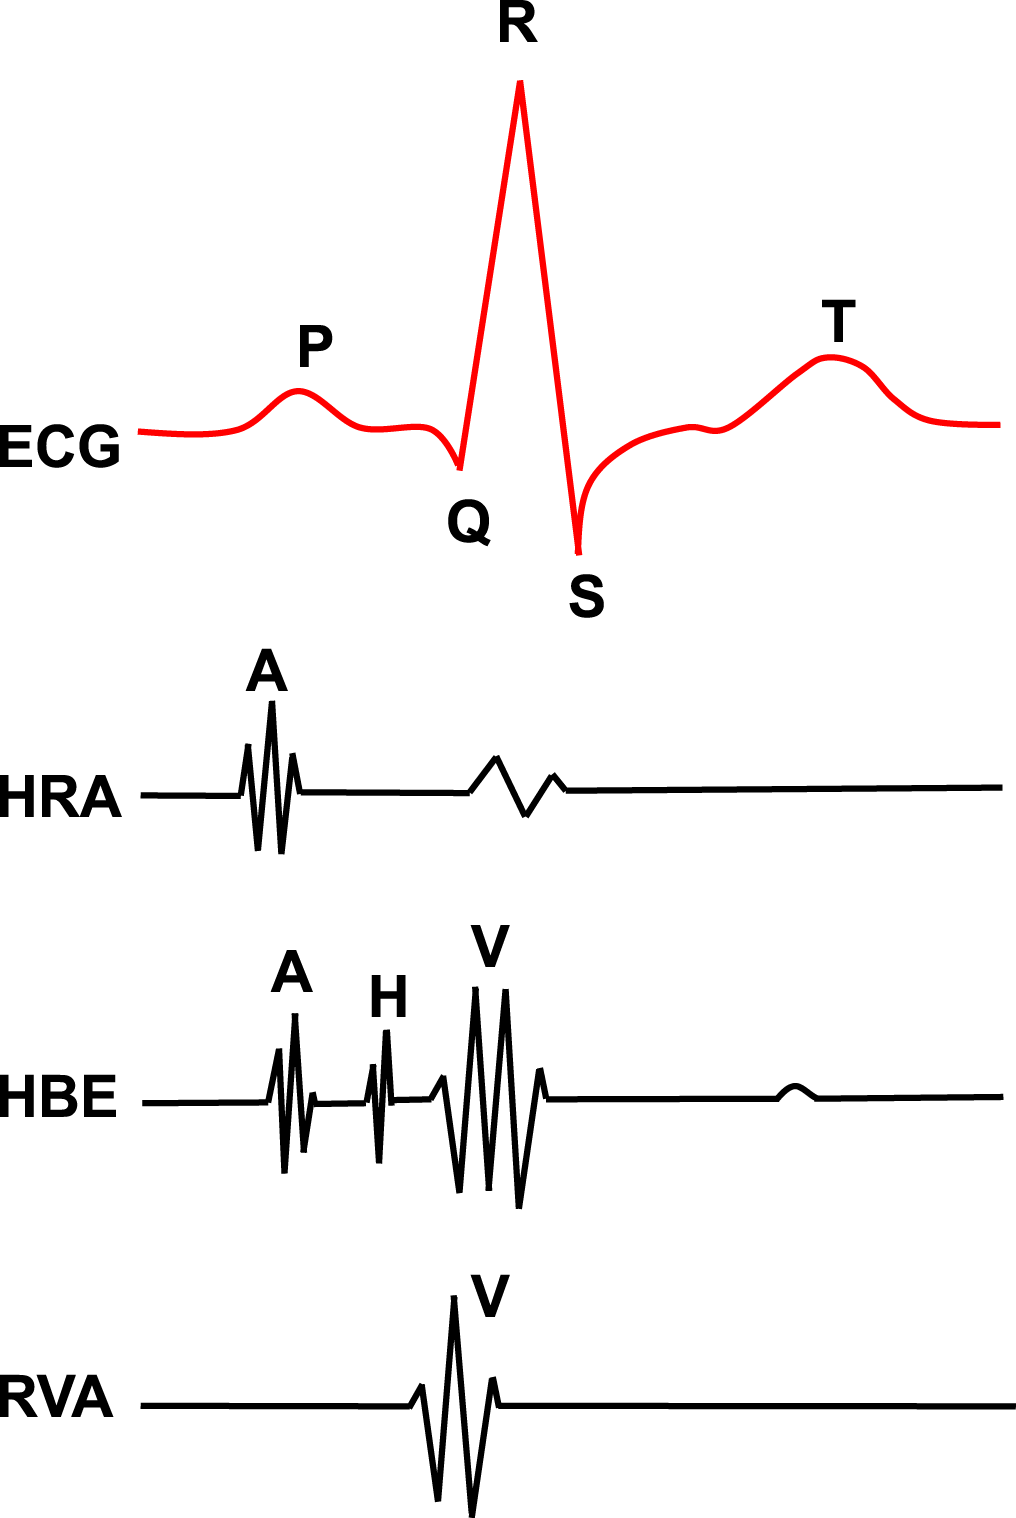
\includegraphics[width=0.2\textwidth]{figs/egm.png}
		%\label{fig:egm}
		%} 
%%\vspace{-10pt}
%\caption{\small (a) Node automaton. Dotted transition is only valid for pacemaker tissue like SA node; (b) Path automaton; (c) Model of the electrical conduction system of the heart using a network of node \& path automata~\cite{vhm_ecrts10}.}
%%\vspace{-15pt}
%\end{figure*} 

%\section{Electrophysiological Testing}
%\Hao{A figure for heart and pacemaker}

%\chapter{Modeling the Physiological Environment}
%\begin{itemize}
	%\item How to encode domain knowledge of the physiological environment into models?
    %\item What are the applications that the models will be used?
    %\item What are the differences in terms of environment models between model checking and simulation?
    %\item How to balance complexity and expressiveness of the model?
%\end{itemize}

%In the following sections, we demonstrate how to construct heart models for closed-loop verification of implantable pacemaker. Note that for two different applications the models are constructed differently as we address their respective requirements for environment models. 


\section{Heart Models For Closed-loop Testing}
%\begin{itemize}
	%\item Why the models at this level have to be deterministic? Where can they be used?
    %\item How electrophysiology reflects the functions of the heart?
    %\item How to encode these knowledge into models?
    %\item Why VHM has the right level of details for pacemaker verification?
    %\item How VHM interacts with pacemaker?
    %
%\end{itemize}
During closed-loop testing, the devices interact with the environment (or its models) under different environmental conditions. The closed-loop executions are monitored and violations of safety/efficacy requirements are reported. In model-based closed-loop testing, the environment models are expected to mimic the behaviors of actual environment and its interaction with the device. Thus the environment models are in general deterministic so that the execution traces are reproducible. Complex dynamics during state transitions also need to be captured to validate violations within longer executions traces. 

\subsection{Modeling Philosophy}

\textbf{Interface to the device: }The pacemaker can only sense and actuate from two locations within the heart, the spatial fidelity requirement for the heart model is thus low. The diagnosis of heart conditions only relies on the timing of the electrical events, thus the behaviors of the model can be reduced to timing only, if a temporal model of the heart is rich enough to represent majority of heart conditions. \\
\textbf{Model expressiveness: }Electrophysiology (EP) is an active field in cardiology based on the fact that the mechanical functions of the heart are largely correlated with the electrical activities. During an EP testing procedure, the physicians diagnose heart conditions by examining the patterns and intervals of local electrical activations (temporal) measured from electrodes placed into different locations of the heart (spatial). 

Based on the analysis above, an EP-based spatial and temporal model of the heart is capable of representing the electrical behaviors of different heart conditions, and more importantly, their interaction with a pacemaker. 

\subsection{Heart Model Components}
We introduce the model components that can be used to configure heart models corresponding to different heart conditions. As introduced in Chapter 2, the action potential of a heart tissue has 3 timing periods during which the tissue responds to external electrical stimuli differently. We use an extended timed-automata formulation (\cite{timed_automata}) to model the timing behaviors of a heart tissue during each cycle. We refer the tissue model as \emph{Node automaton} and \figref{node_automata} shows the structure of a node automaton $i$. 3 states correspond to 3 timing periods of the action potential. From \textsf{Rest} state, the node can either self activate or activated by external stimuli (Act\_node) and go to \textsf{ERP} state. During \textsf{ERP} state the node does not respond to external stimuli (blocked). During \textsf{RRP} state, the node can still be activated and go to \textsf{ERP} state, however the ERP period and the conduction delay of the tissue are affected by the "earliness" of the activation arrived during the RRP period, which is tracked by a shared variable $C(i)$. The new ERP period is determined by a function over clock value $g(f(t))$ which mimic the beat-to-beat dynamics described in \cite{josephson}. The function $g$ and $f$ are given by:
\begin{equation} \label{factor}
						f(t) = 1-t/Trrp
						\end{equation}
and
%  The AV node has a different profile than the other tissue. The ERP period increases rather than decreases when activated during its RRP (~\cite{josephson}).
\begin{equation} \label{earliness_noAV}
						g(x) = \left\{
						\begin{array}{lr}
						
						T_{min}+(1-(1-x)^3)\cdot (T_{max}-T_{min}), i=AV\\
						T_{min}+(1-x^3)\cdot (T_{max}-T_{min}),i\neq AV
			
						
						\end{array}
						\right.
						\end{equation}  
where $T_{min}$ and $T_{max}$ are the minimum and maximum value for \emph{Terp} of the tissue.
\begin{figure*}[!t]
\centering
		\subfigure [\small]{			
		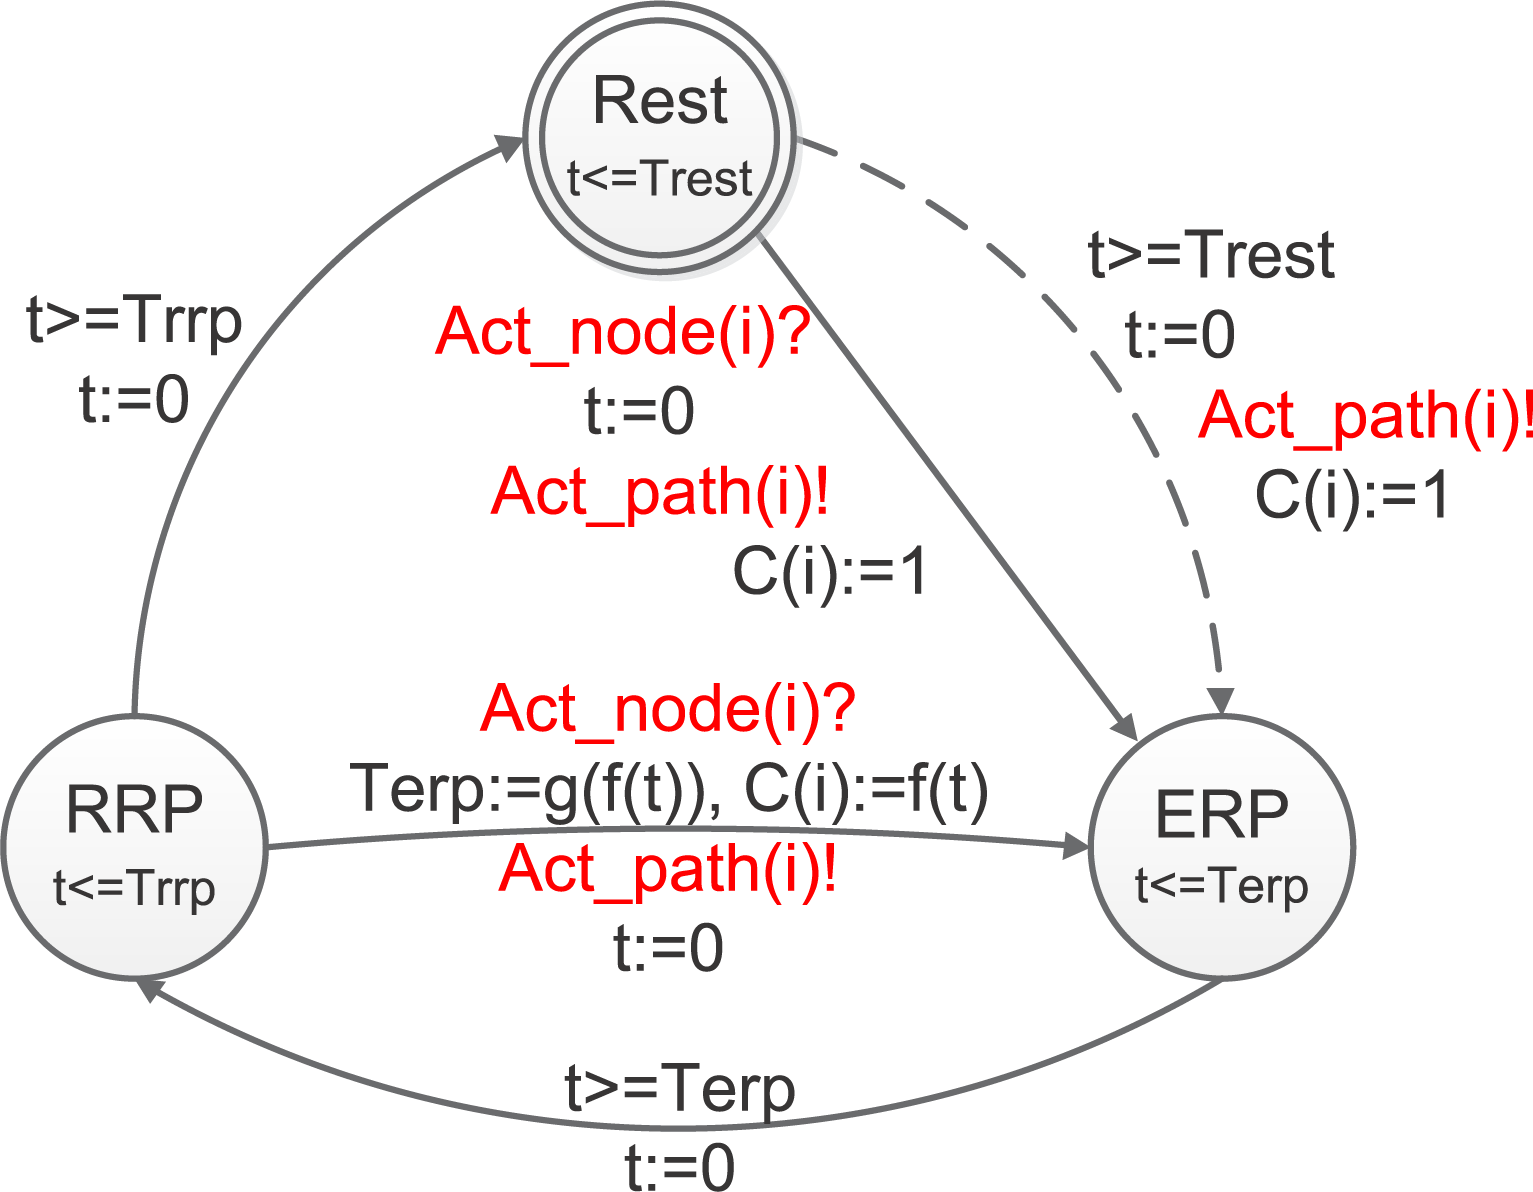
\includegraphics[width=0.35\textwidth]{figs/node_aut.png}
		\label{fig:node_automata}
		} 
%	\hspace{.1in}%
		\subfigure [\small] 
		{
		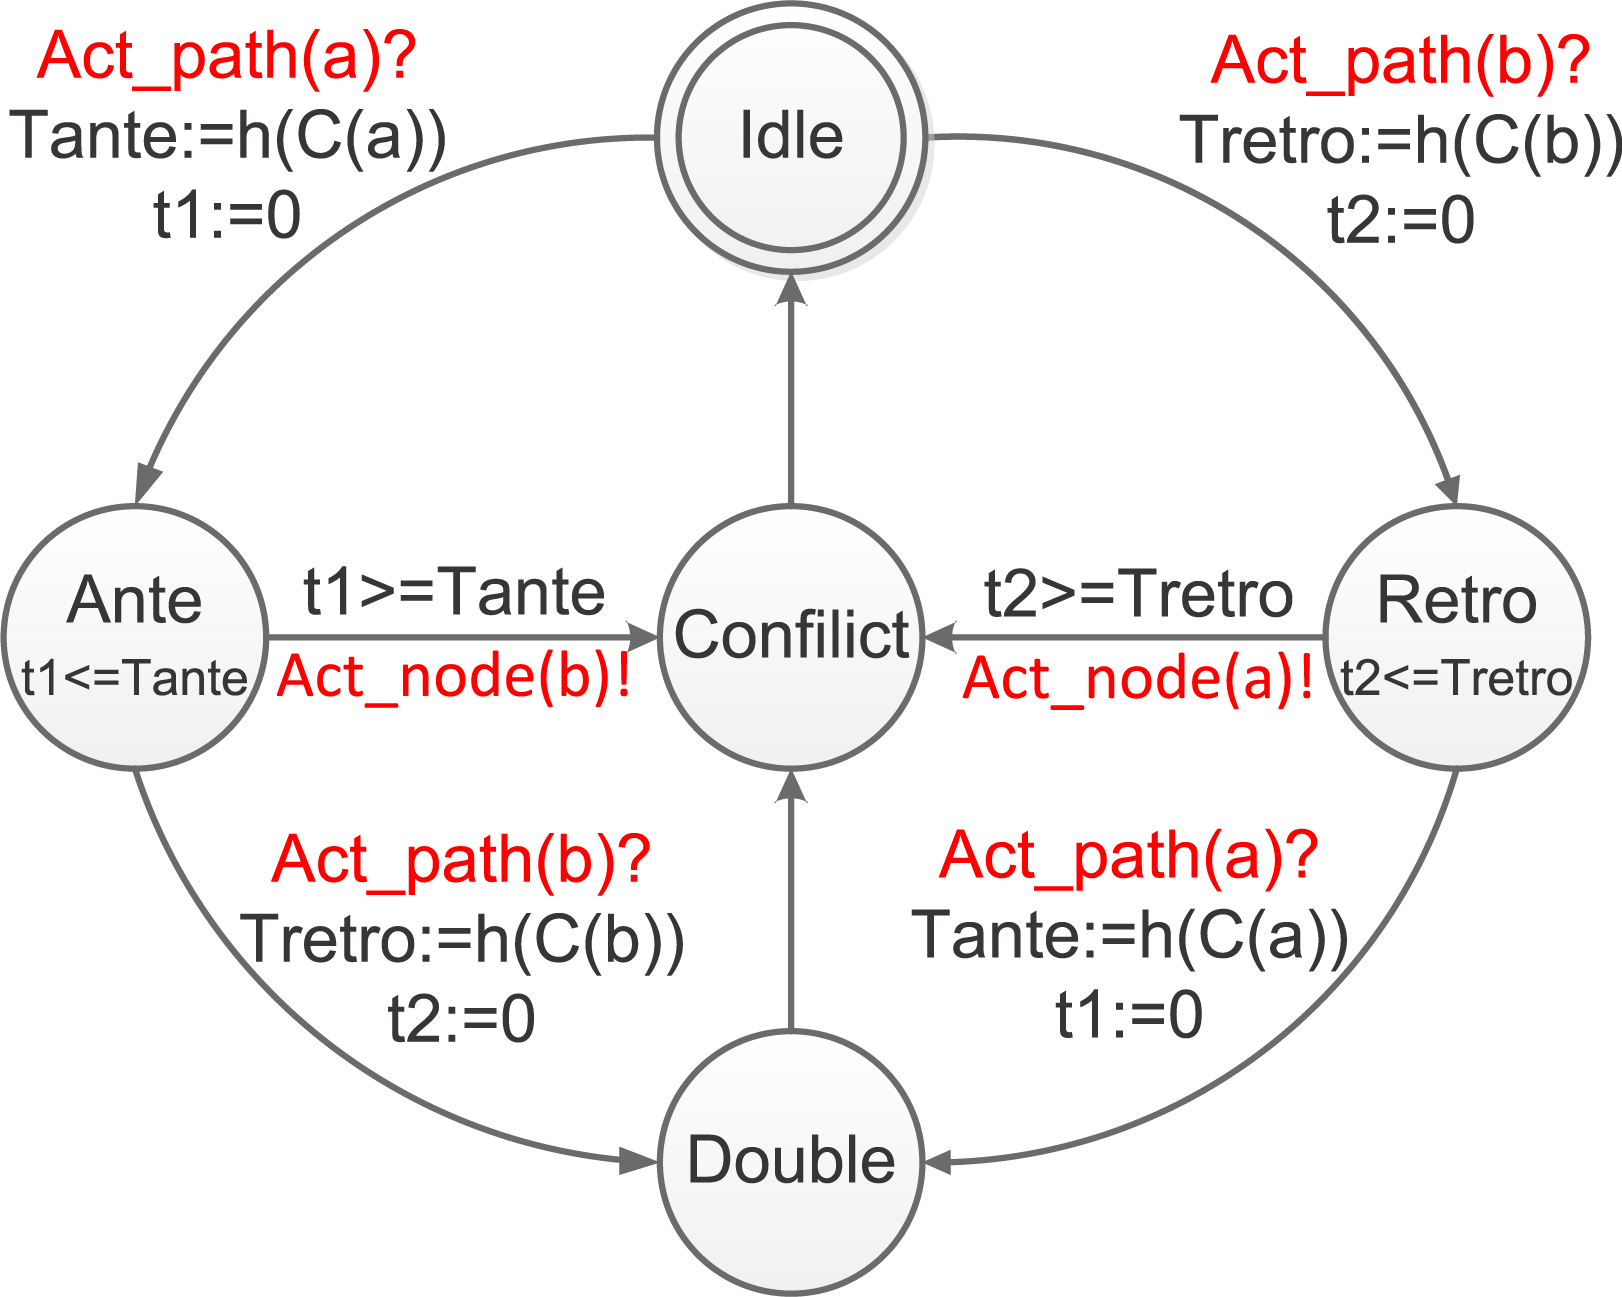
\includegraphics[width=0.35\textwidth]{figs/path_aut.png}
		\label{fig:path_automata}
		} 
		\subfigure [\small] 
		{
		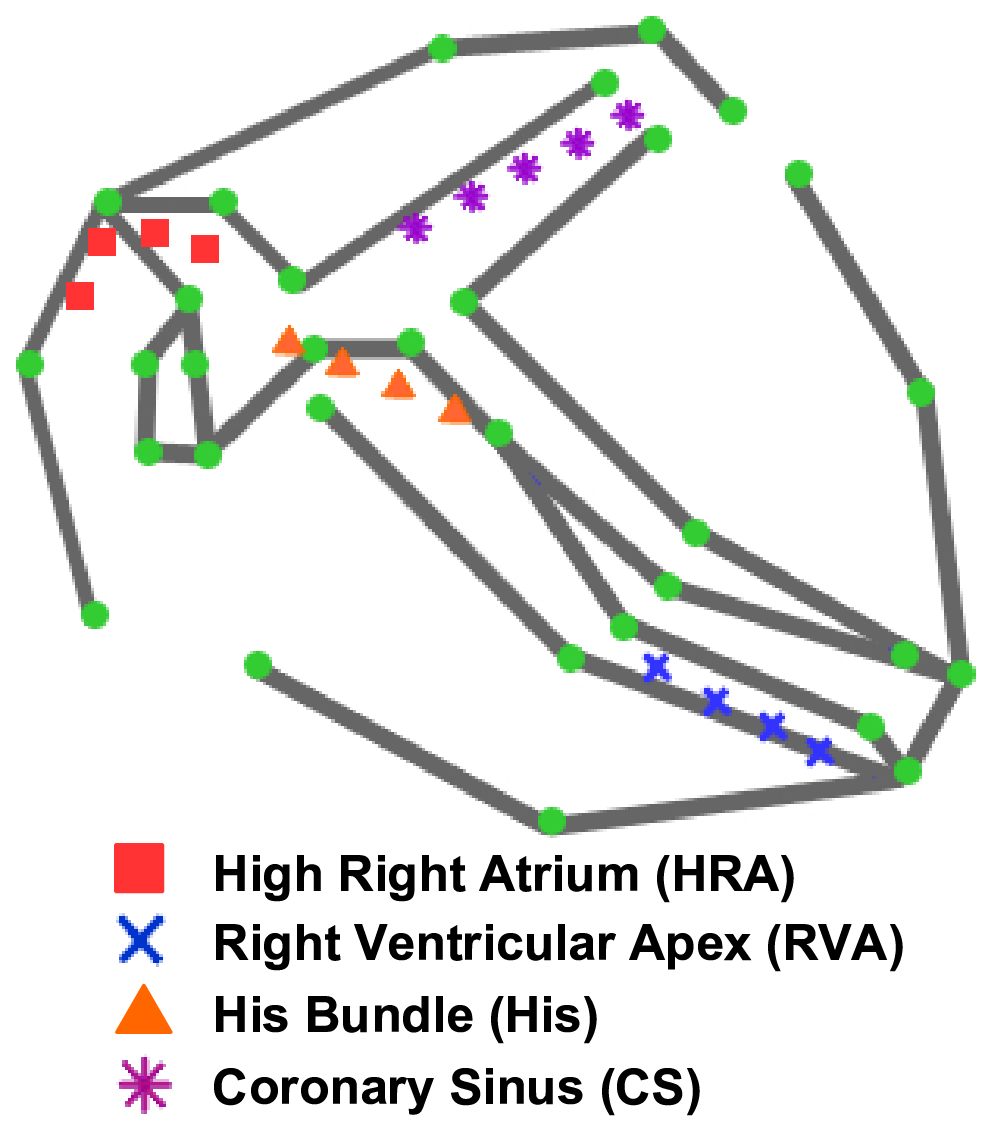
\includegraphics[width=0.2\textwidth]{figs/gen_setup.png}
		\label{fig:general_setup}
		} 
\label{fig:h_automatas}
%\vspace{-10pt}
\caption{\small (a) Node automaton. Dotted transition is only valid for pacemaker tissue like SA node; (b) Path automaton; (c) Model of the electrical conduction system of the heart using a network of node \& path automata ~\cite{vhm_ecrts10}.}
%\vspace{-15pt}
\end{figure*} 

Due to the limited number of observable points within the heart, modeling every tissue of the heart and its full anatomy is unnecessary and unfeasible. In our heart models, only self-activating tissue and key hubs of the electrical conduction system are modeled as node automata. The electrical conduction through the tissue between nodes are abstracted using \emph{path automata}. The path automata can be used to represent structural or topological (functional) electrical connections between nodes. \figref{path_automata} shows a path automaton connecting node a and b.

The initial state of a path automaton is \emph{Idle}, which corresponds to no conduction. The states corresponding to the two conduction directions are named after the physiological terms: Antegrade (Ante) and Retrograde (Retro). These states can be intuitively described as forward and backward conductions. If \emph{Act\_path} event is received from one of the nodes connected to it, the a transition to \emph{Ante} or \emph{Retro} state correspondingly will occur in the path automaton. At the same time the clock invariant of the state is modified according to the shared variable \emph{C(a/b)}. This corresponds to the change of the conduction delay that is caused by the early activation. Similar to node automaton, the changing trend is extracted from clinical data and the function $h$ is defined as:
\begin{equation} 
						h(c) = \left\{
						\begin{array}{lr}
						
						path\_len/v\cdot (1+3c), i=AV\\
						path\_len/v\cdot (1+3c^2), i\neq AV
						\end{array}
						\right.
						\end{equation}
where $path\_len$ denotes the length of the path and $v$ is the conduction velocity.

After \emph{Tante} or \emph{Tretro} time expires, the path automaton sends out \emph{Act\_node(b)} or \emph{Act\_node(a)} respectively. A transition to \emph{Conflict} state occurs followed by the transition to \emph{Idle} state. The intermediate state \emph{Conflict} is designed to prevent back-flow, where the path is activated by the node \emph{b} it has just activated. If during \emph{Ante} or \emph{Retro} state another \emph{Act\_path} event is received from the other node connected to the path automaton, a transition to \emph{Double} state will occur, corresponding to the two-way conduction. In this case, the activation signals eventually cancel each other and the transition to \emph{Idle} state is taken.

\subsection{Modeling the Electrical Conduction System}
The node and path automata are the basic building blocks for heart modeling. Different hearts under different conditions have different timing parameters and/or different conduction topology. We connect node and path automata with different timing parameters into a network to represent different heart conditions. (\figref{general_setup}) 

\subsection{Interaction With The Heart Model}
In EP testing and pacemaker application, the local electrical activities, measured as electrogram (EGM) signals, are used to diagnose heart conditions. During heart model construction, we can assign a node automaton at electrode locations and the transitions to the ERP state can be used to represent the local activation events. In a more general setup where electrodes are assigned anywhere within the heart model, a probe model is designed to generate synthetic EGM signals using temporal information and spatial information from the network of node and path automata. \figref{egm_s} shows the morphology of EGM signal changes with different conduction velocity and probe configurations. Due to space limitation, detailed description of the probe model can be found in \cite{vhm_embc11}.

\begin{figure}[!t]
\center
%\vspace{-15pt}
		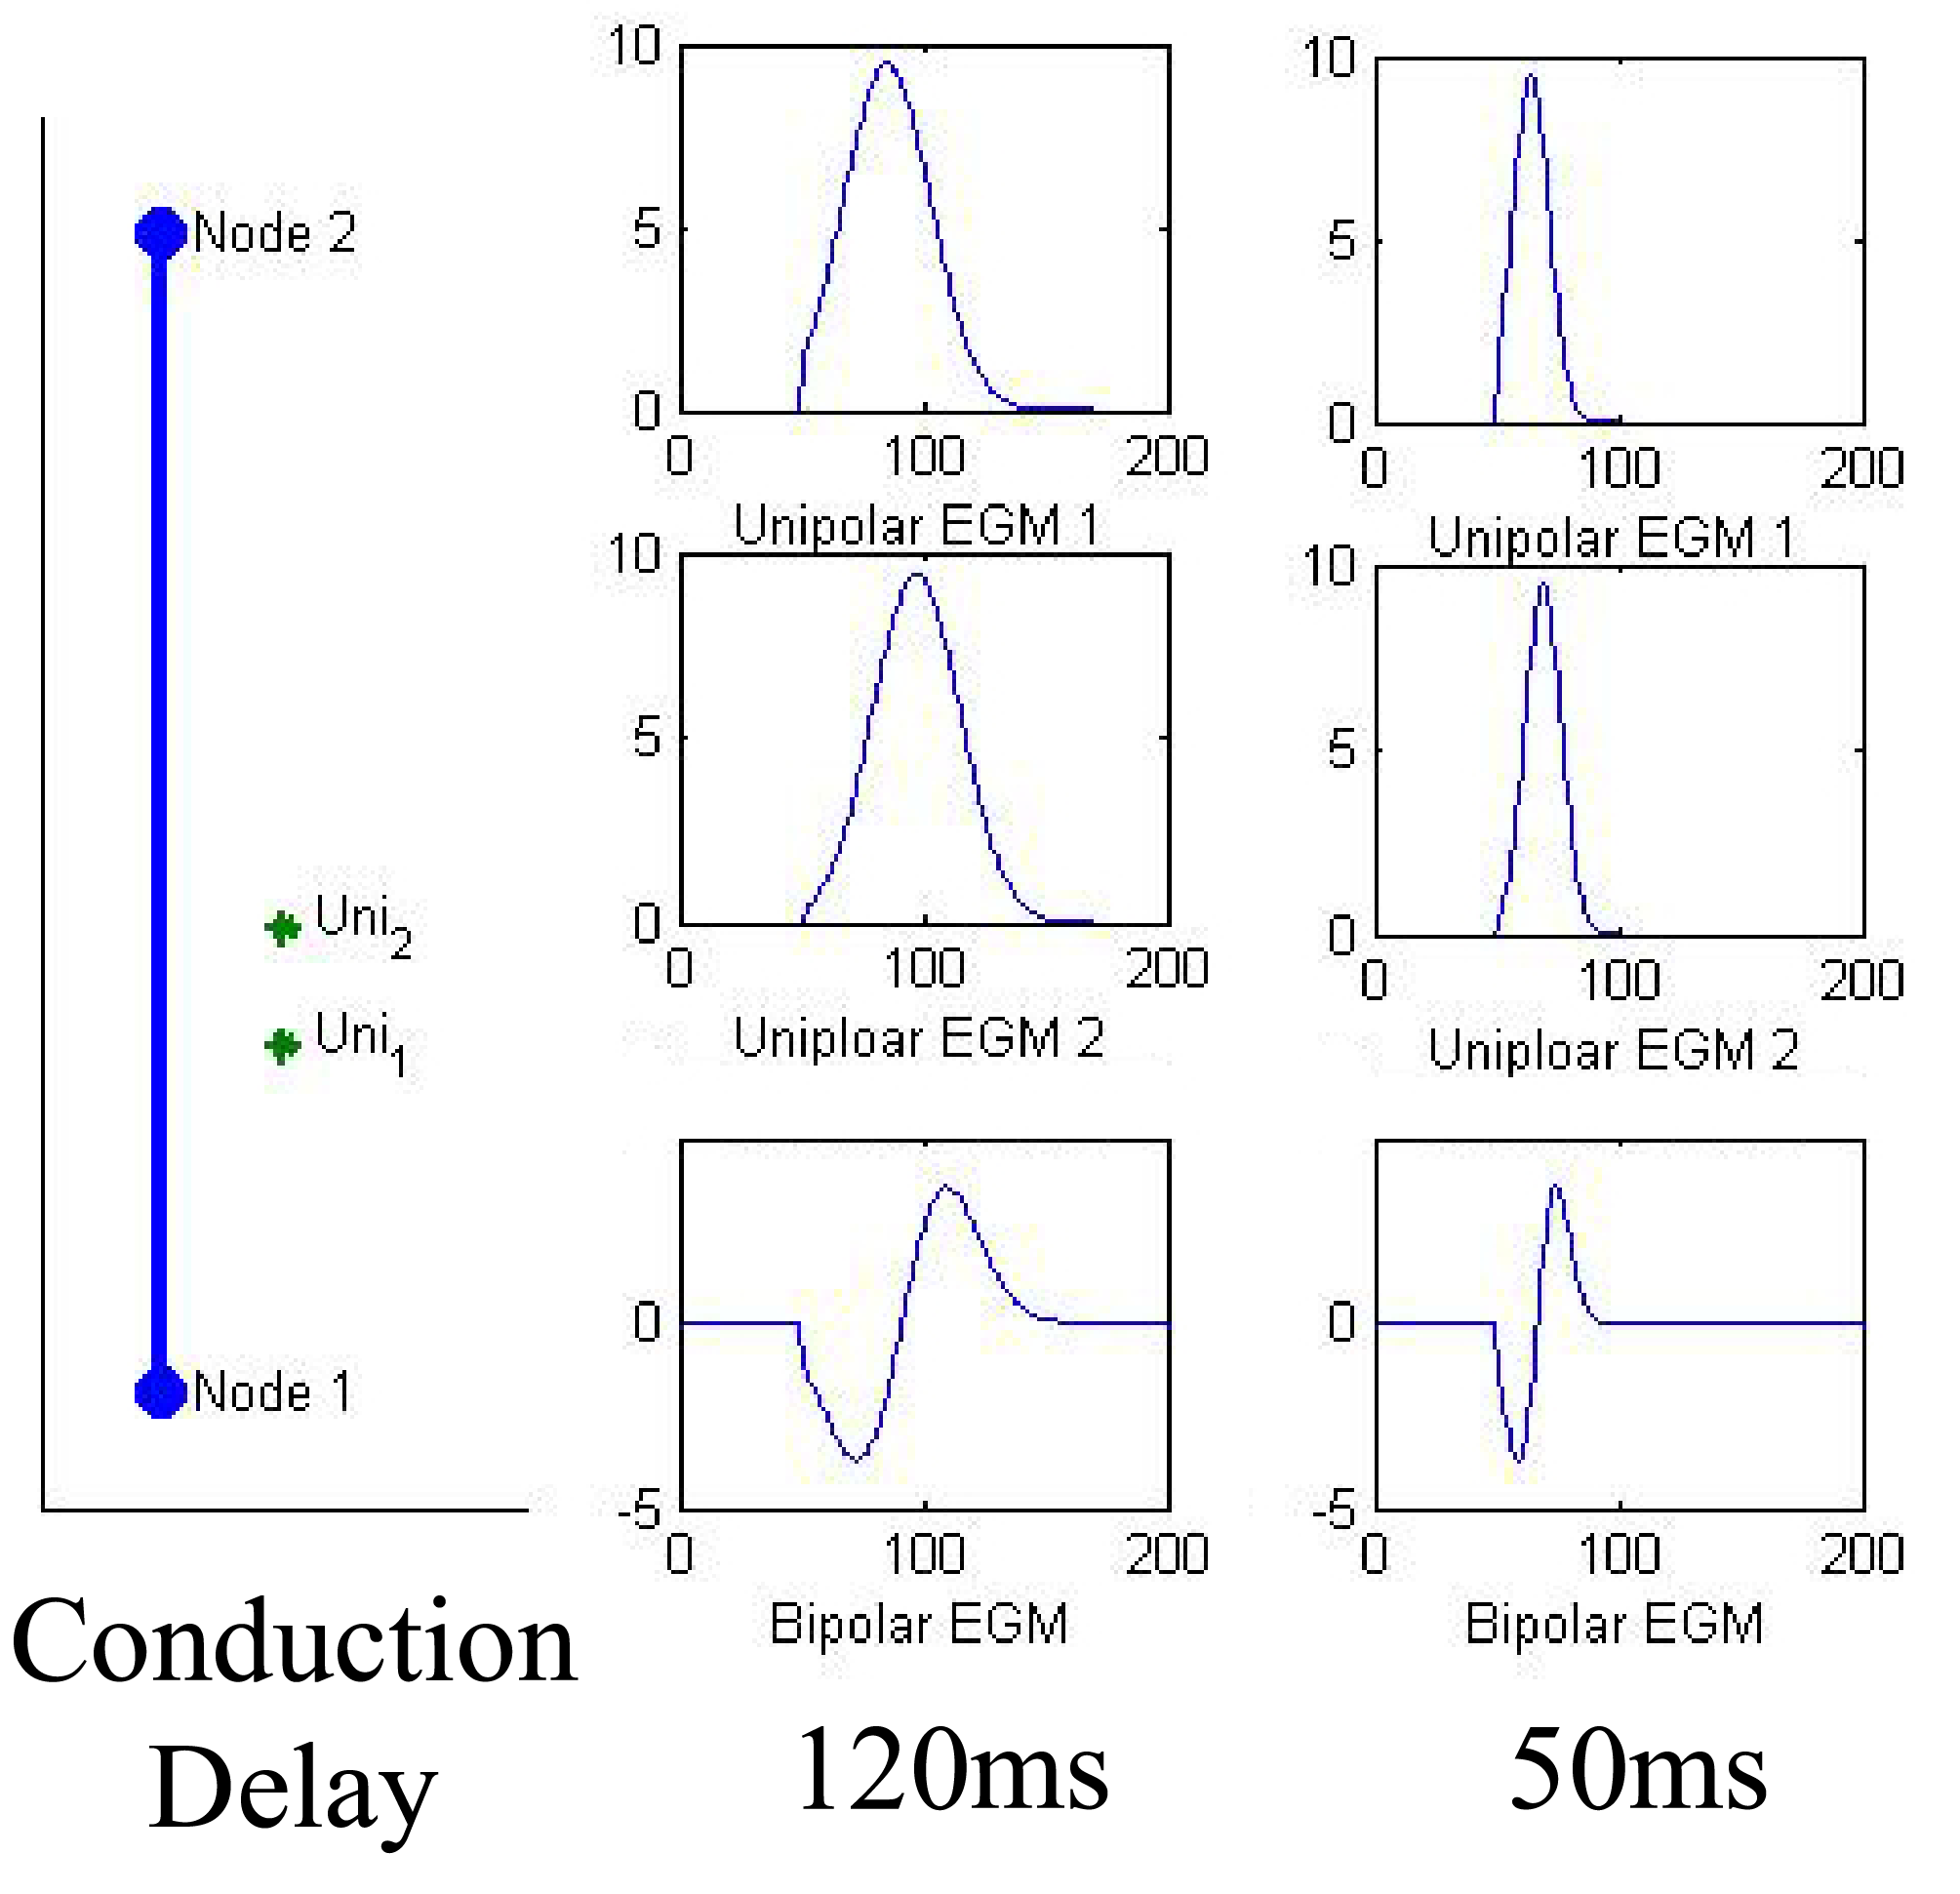
\includegraphics[width=0.45\textwidth]{figs/fig7.png}
%\vspace{-10pt}
\caption{The influence of conduction velocity and probe configuration on the EGM morphology. The left columns show the placement of probes in relation to the path; the right columns show the functional EGM.}
\label{fig:egm_s}
%\vspace{-15pt}
\end{figure}

\section{Non-deterministic Models for Closed-loop Model Checking}
%\begin{itemize}
	%\item What does nondeterminism do? Where can these model be used?
    %\item How to replace complex dynamics of the deterministic models with nondeterminism?
    %\item What are the abstraction rules that can be applied to the heart models and what are their physiological basis?
    %\item How to encode the information loss during each abstraction steps?
%\end{itemize}
During closed-loop model checking, the whole closed-loop state space of the device and the environment is mathematically explored against physiological requirements. The  ideal environment models should be: 1) simple enough to avoid the state space explosion problem, 2) general enough to cover possible physiological conditions, 3) complex enough to represent any specific physiological conditions. It is obvious that no single model can achieve all 3 properties. A rigorous framework should be adapted so that appropriate models are selected for corresponding requirement.
\subsection{Modeling Philosophy}
\textbf{Model Formalism: }Choosing an appropriate formalism for the physiological models is important as the formalism determines the closed-loop state space and the feasibility/efficiency to do model checking. Pacemaker utilize the timing of local electrical events to diagnose heart conditions. It is therefore intuitive to use timed-automata models of the heart. Timed-automata is also compatible with model checking tools like UPPAAL (\cite{uppaal_tut}) so that the whole closed-loop state space can be explored.\\
\textbf{Model Coverage: }Pacemakers are designed to treat bradycardia, however not only should the pacemakers maintain appropriate heart rate when the intrinsic rate is low, but also shall not degenerate other heart conditions. Even for the same patient the condition also changes over time that has to be taken into account. In order to achieve safety across all possible heart conditions, the heart models used during closed-loop verification should be able to cover all possible heart behaviors, more precisely, their mapping to pacemaker inputs. Over-approximation (\cite{CEGAR}) with non-determinism can be used to simplify model structure while covering larger variety of environmental behaviors. Techniques like model-checking can then be used to examine the whole closed-loop state space for property violations.\\ 
\textbf{Ambiguity Due To Low Sensing Capability: }The sensing resolution of pacemakers is low, in terms of the number of sensing location (2 leads), as well as the information obtained from each sensing location (binary events). If abstraction rules utilize the fact that different heart conditions may generate exactly the same input sequence to the pacemaker, there will be ambiguities on concretizing abstract closed-loop executions. For certain conditional requirements, it is important to differentiate all possible concrete executions corresponding to an abstract execution. As the result, the heart model(s) should have the capability to differentiate these heart conditions when verifying certain properties.\\
\textbf{Information Lose During Abstraction: }While over-approximation achieves simplicity and coverage, it also inevitably introduces invalid behaviors into the model which can cause false-negatives and false-positives during model checking. To solve this problem, more refined models of the heart should be available which can differentiate and eliminate invalid executions when necessary to avoid false-positives.

The most challenging aspect during closed-loop model checking is environment model abstraction and refinement. In \cite{STTT13} we developed a series of heart model abstractions at various abstraction levels. The models are abstracted using abstraction rules derived from physiological knowledge, thus ensuring that each abstraction step covers more physiological conditions. The models in adjacent abstraction levels also satisfy \textsf{timed-simulation} relationship (\cite{simulation}) to ensure complete coverage in the more abstract model. In the rest of the section, we briefly discuss the modeling process and the domain knowledge used. The detailed abstraction and proof for simulation relationship can be found in \cite{STTT13}.
\begin{figure}[!t]
\center
%\vspace{-10pt}
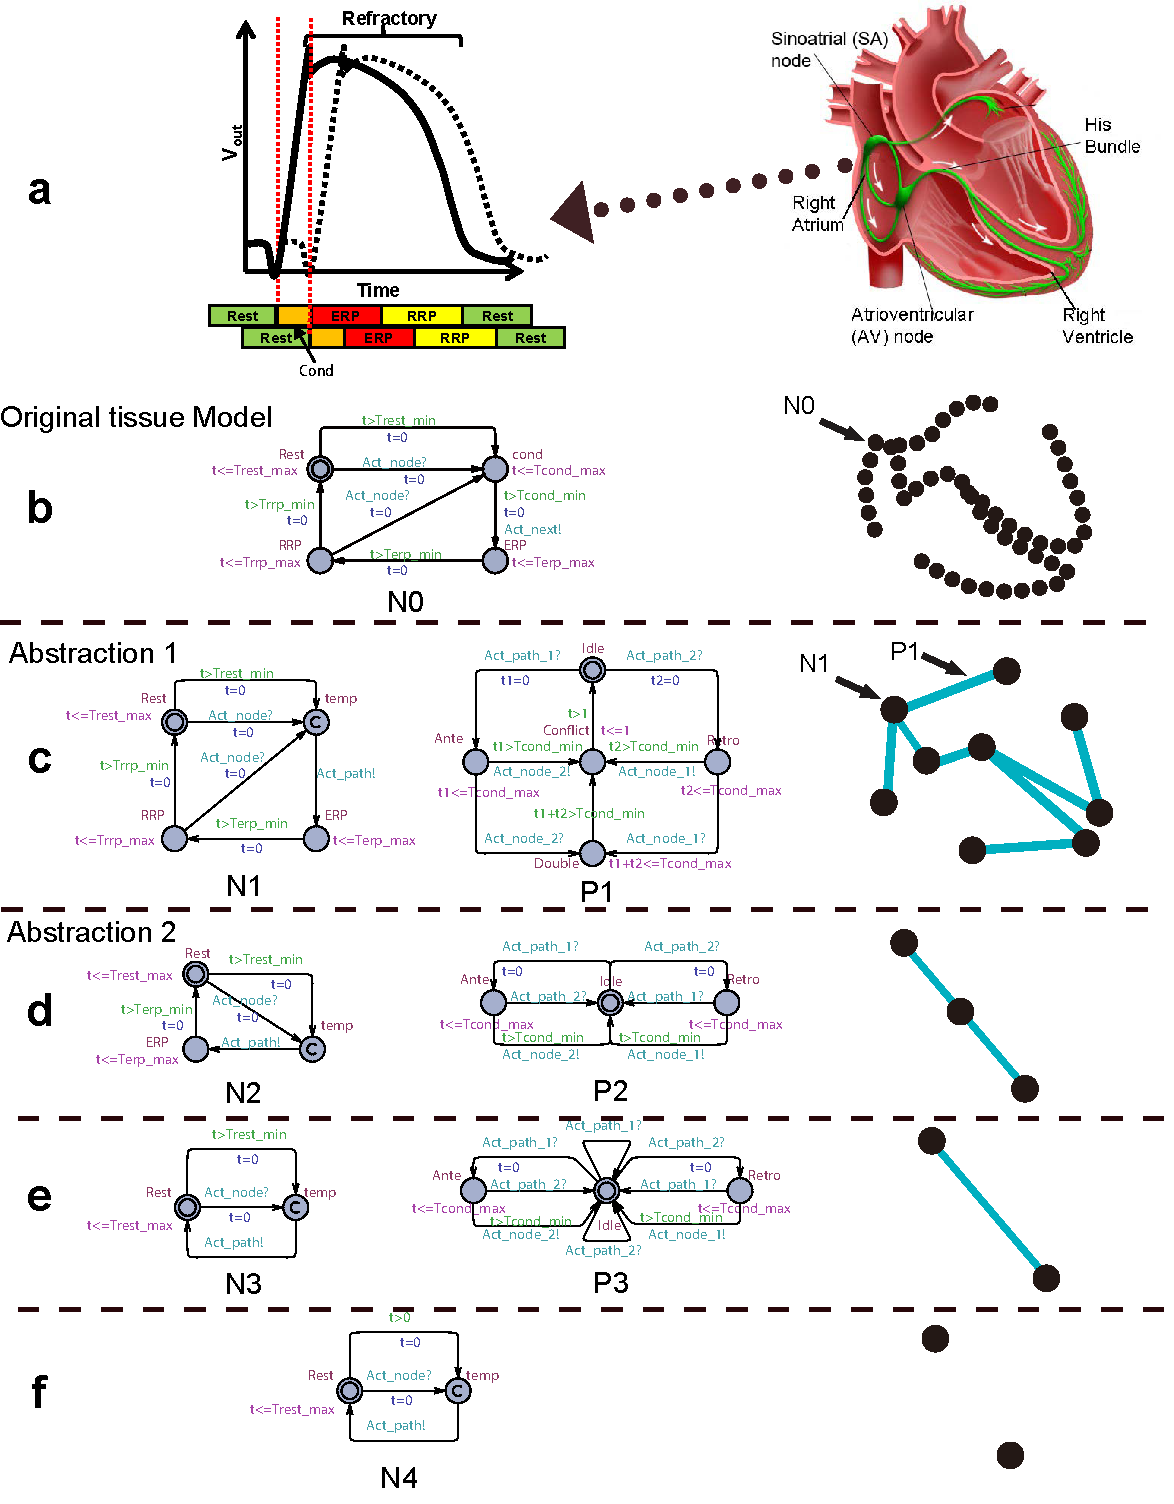
\includegraphics[width=0.9\textwidth]{figs/Heart_abs.pdf}
%\vspace{-10pt}
\caption{(a) The generation of Action potential; (b) Action potential; (c1) The second activation arrived during ERP; (c2) Arrived during RRP; (c3) Arrived after refractory. (\cite{STTT13})}
\label{fig:HM_abs}
%\vspace{-10pt}
\end{figure} 
\subsection{Initial Abstraction}
For the initial heart model, spatially we assume that every heart tissue are modeled. Temporally we model each heart tissue as an automaton $N0$ shown in \figref{HM_abs}.b. The beat-to-beat dynamics of heart tissue discussed in the last section is abstracted using non-determinism, as the ERP period and conduction delay of the tissue are non-deterministically chosen from ranges instead of deterministic functions. The model covers all possible timing behaviors of a heart tissue. 

\subsection{Abstract Conduction Delays With Paths}
At the first abstraction step, we seperate the conduction delay (modeled by the cond state in $N0$) from the new node automata $N1$ and model the conduction between two nodes using path automaton $P1$. Since the beat-to-beat dynamics are abstracted with non-determinism, the RRP state is merged with the Rest state in $N1$. 

we only model the following kinds of heart tissue with node automata and abstract other heart tissue with path automata:
\begin{itemize}
	\item Self-depolarizing tissue
    \item Tissue with long ERP period
    \item Tissue forming conduction loops
\end{itemize}

\subsection{Merging}
abstract heart tissue
% \subsubsection{Abstracting Beat-to-beat Dynamics}
% \subsubsection{Abstracting Conduction Delays with Path}
% \subsubsection{Merging Activation-generating Nodes}
% \subsubsection{Replace ERP Blocking With Non-deterministic Conduction}
% \subsubsection{Replace }



\chapter{Identifying and Validating the Environment Model }

Physiological models are developed to represent certain clinical conditions common across a population of patients, or the condition of a specific patient. Consequently, the structure of the model and corresponding parameters have to be identified. This information can be obtained from electrogram data collected during medical procedures and from physiological literature in which population data has been analyzed and summarized. Due to limited interactions with the patient (e.g. during a device implantation procedure or an ablation procedure), currently the quality and quantity of patient-specific physiological data is sparse as there is generally not enough information to identify all the parameters in the model.  A model with the spatio-temporal structure that is similar to the conduction patterns in the heart helps simplify the process of identifying the model parameters. A rigorous procedure for the model identification step is an important contributor to the model validation step. In this chapter, we aim to answer the following questions:
%%It is essential to choose the right level of abstraction so that the model is identifiable (to a large extent). Having physiological correspondence for the model structure and parameters can also simplify the identification process. 

\begin{itemize}
	\vspace{-5pt}
	\item What is the importance of model identification for closed-loop simulation and model checking?
	\vspace{-5pt}
    	\item How are models identified from patient data and patient population parameters?
\end{itemize}

In the following section, we briefly discuss our model identification effort for heart models used in two closed-loop verification applications, and their corresponding challenges. This is followed by the procedures to validate the heart models before they are used for closed-loop verification and testing of the pacemaker.
\begin{figure}[!t]
\centering
		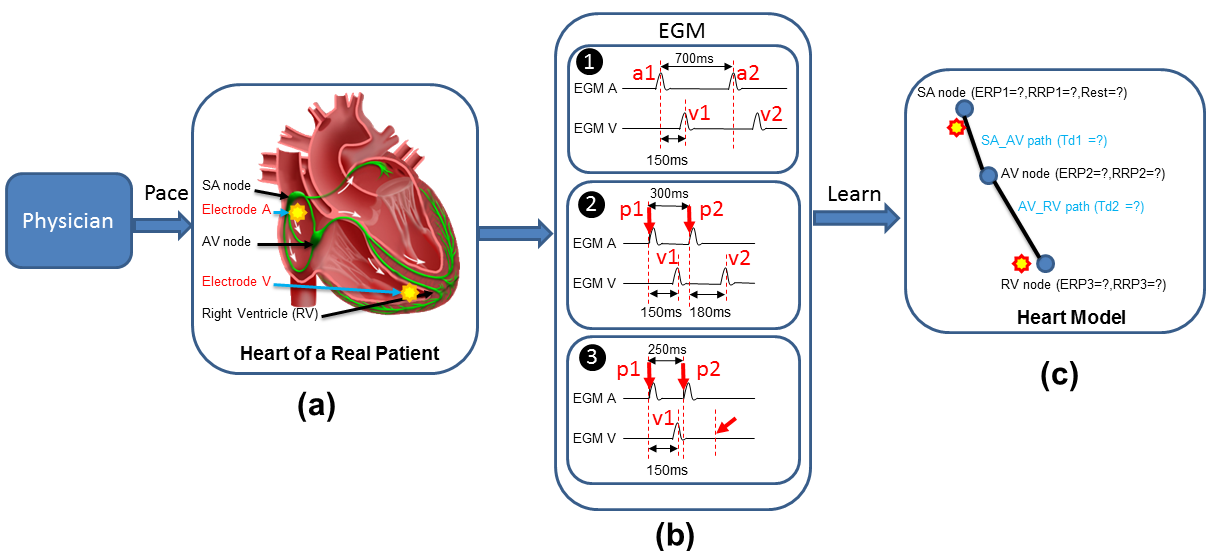
\includegraphics[width=0.9  \textwidth]{figs/modelID.png}
		
%\vspace{-10pt}
\caption{\small (a) The illustration of the probe locations. (b) Multiple pacing sequences with different timing outcomes. (c) The heart model with undecided parameters}
\label{fig:modelID}
%\vspace{-15pt}
\end{figure} 

\section{Heart Model Identification for Closed-loop Simulation}
In closed-loop simulation, a deterministic heart model should be identified to represent a specific patient under a certain heart condition. The constraints for model parameters can be obtained from patient data with \emph{Electrophysiological (EP) Testing}. During EP testing, the physician delivers electrical pacing sequences from electrodes placed inside the patient's heart to instigate responses along fast and slow conduction pathways. The observed patterns and timing of electrical events are used to extract extract conduction and propagation properties of different tissue regions across the myocardium. Since the goal for any EP testing procedure is not to determine all the timing parameters for a patient, the amount of parameters that can be identified from the patient data is limited.    

\figref{modelID} illustrates how timing parameters can be extracted during an EP testing procedure. \figref{modelID}(a) shows a setup with two electrodes placed in the right atrium and right ventricle of the heart respectively. EGM signals can be measured from these two electrodes (\figref{modelID}(b)). The physician delivers long and short interval pacing sequences through the electrodes which may trigger different responses along different conduction pathways from the patient's heart. \figref{modelID}(c) shows a heart model structure with unknown parameter values. By analyzing the \emph{timing} and \emph{pattern} of the EGM signals we extract constraints on the heart model parameters. In EGM sequence 1, the interval between two intrinsic activations $a1$ and $a2$ in EGM A is 700ms, so we have:
$$ERP1+RRP1+Rest=700ms$$
The interval between $a1$ and $v1$ is 150ms, so we have:
$$Td1+Td2=150ms$$
In EGM sequence 2, the pacing interval from Electrode A is 300ms. By observing that the interval between $p1-v1$ is less than the interval between $p2-v2$, we know that $p2$ arrives during the RRP period of the AV node. So we have:
$$ERP1+RRP1\leq 300ms$$
In EGM sequence 3, the pacing interval is further reduced to 250ms. There is no $v2$ corresponding to $p2$, indicating $p2$ arrives during the ERP period of the AV node. So we have:
$$ERP1\leq 250ms$$
Each experiment provides additional time constraints for model parameters. By systematically conducting experiments certain model parameters can be uniquely identified within a relatively tight range. However, even with simplified model structure like the one in the example, not all model parameters can be uniquely identified due to limited number of electrodes and limited number of experiments during a real procedure.






\subsection{Heart Model Identification in Closed-loop Model Checking}
In model checking, the heart models have simpler structure and fewer parameters due to non-deterministic abstraction. The placement and connectivity of nodes and paths in the heart models are developed to be consistent with EP practice. This way, each node and path automata and their timing parameters have physiological correspondence to parameters found in literature (\figref{intervals}). The range for non-deterministic parameters directly corresponds to the range for possible values of the respective physiological parameters. Therefore, model identification for model checking is much simpler and . 

\begin{figure}[!t]
\centering
		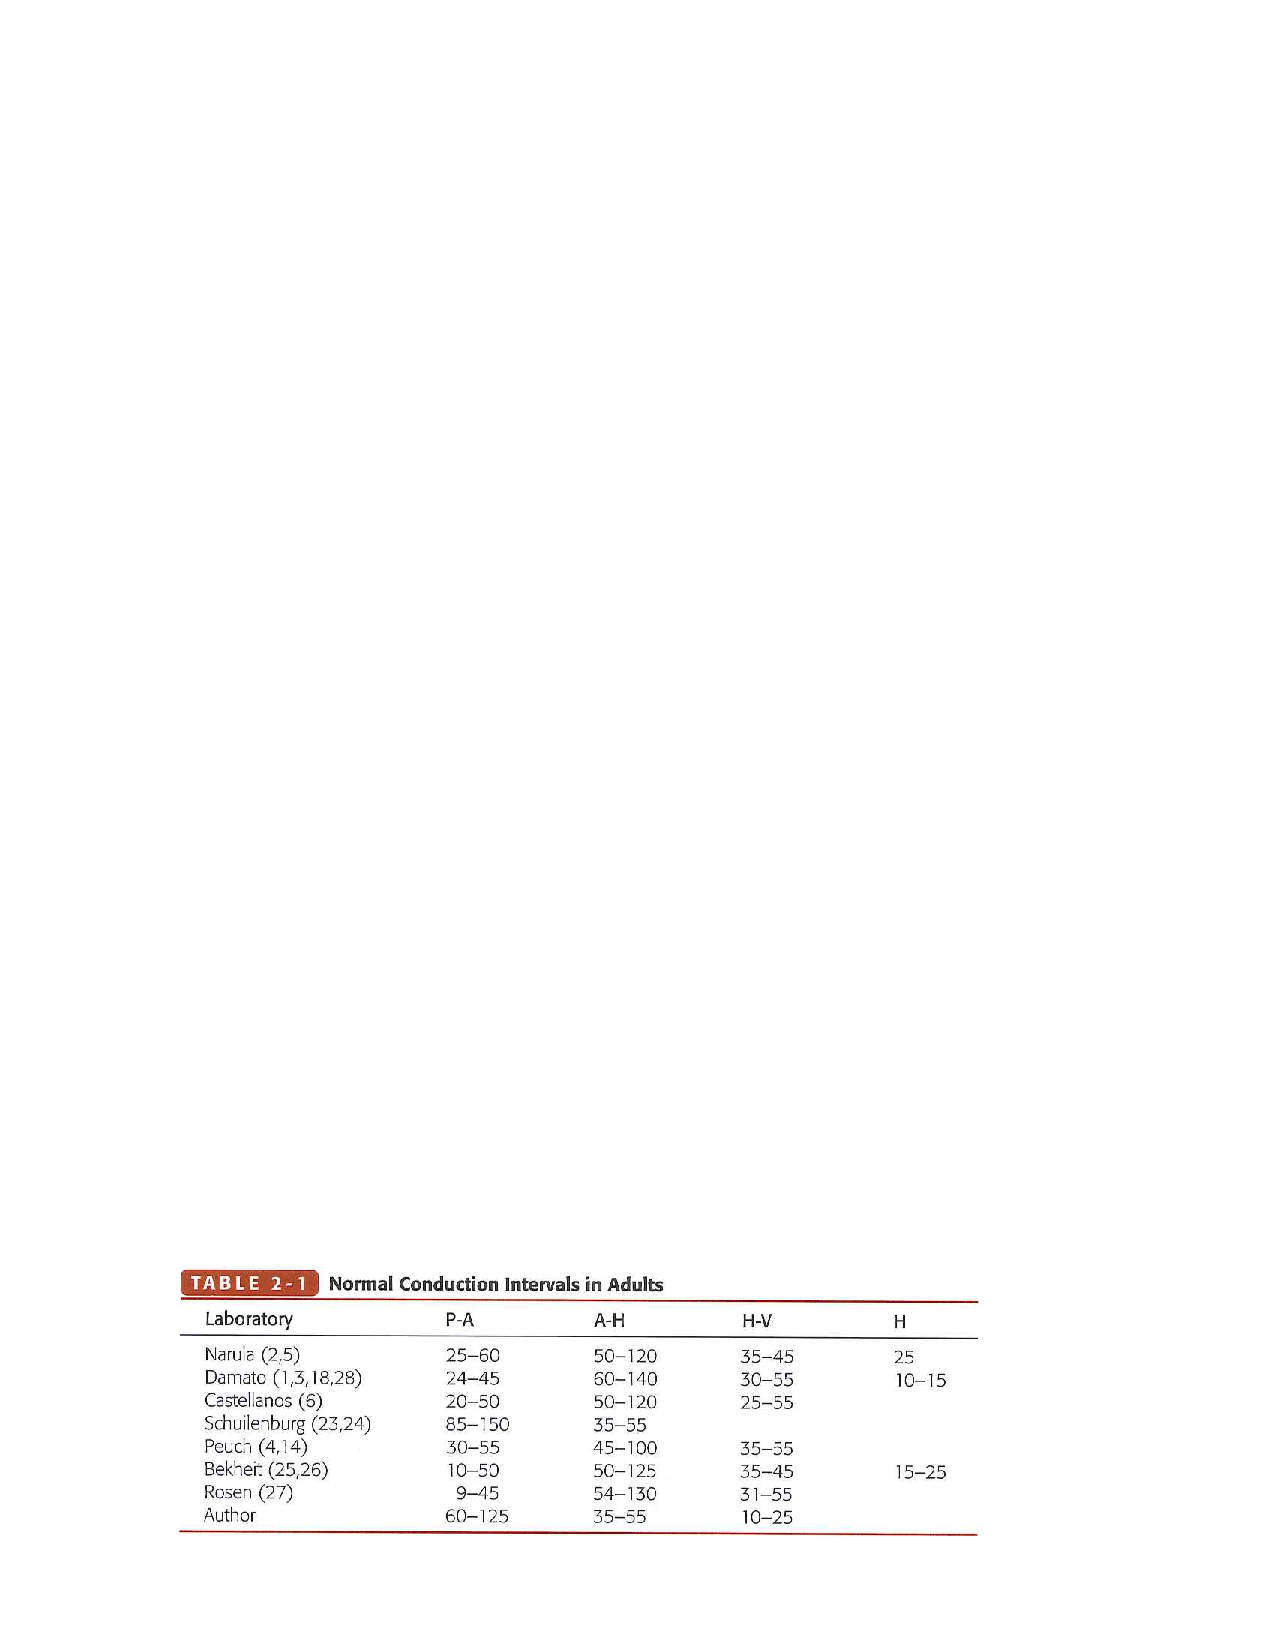
\includegraphics[width=0.8\textwidth]{figs/intervals.pdf}
		
%\vspace{-10pt}
\caption{\small Timing intervals measured during clinical studies \cite{josephson}}
\label{fig:intervals}
%\vspace{-15pt}
\end{figure} 



%%%%%%%%%%%%%%%%%%%%%%%%%%%%%%%%%%%%%
%%%%%%%%%%%%%%%%%%%%%%%%%%%%%%%%%%%%%


\section{Validating the Environment Model}
%The validity of the environment models affects the validity of the closed-loop verification results. 
Since models are approximations of the actual environment, there are always discrepancies between the model and the actual patient (group). The challenge then is to evaluate the confidence in the safety guarantees that model-based closed-loop verification can provide. The metric and process to validate the environment model is different for the two applications of heart modeling: in closed-loop model checking, the model's \textbf{coverage} on environmental behaviors is more important, while in closed-loop simulation, the \textbf{accuracy} of the model is more important. In this chapter, we aim to answer the following questions and use our heart models as examples to demonstrate different validation procedures which improve the fidelity of the environment model. 
\begin{itemize}
	\vspace{-5pt}
	\item What are the different methods to validate physiological models?
	\vspace{-5pt}
	\item How much confidence is sufficient from the model validation process?
\end{itemize}

\subsection{Validating Models for Closed-loop Simulation}
A physiological model is considered valid for closed-loop simulation if (a) it is capable of generating the same output as the patient given the same input; and (b) it is general enough to represent other patients with similar conditions by adjusting its parameters. The second point is to ensure that the model successfully captures the underlying mechanism instead of over-fitting the data. In the following example we demonstrate the capability of our heart models to model certain heart conditions according to the mechanism described in physiological literature, and the model exhibits expected output given the proposed inputs.

%To use a physiological model for closed-loop simulation, there are two levels of validity: 1) model a patient with certain heart condition, 2) model a \em ph{specific} patient with certain heart condition. Level 1 validity ensures that the model successfully models the underlying mechanism of the heart condition, while level 2 validity guarantees the capability of the model to generate same data as the corresponding patient given the same input. Note that satisfying level 2 without satisfying level 1 may result in over-fitting.
\begin{figure}[!t]
\centering
		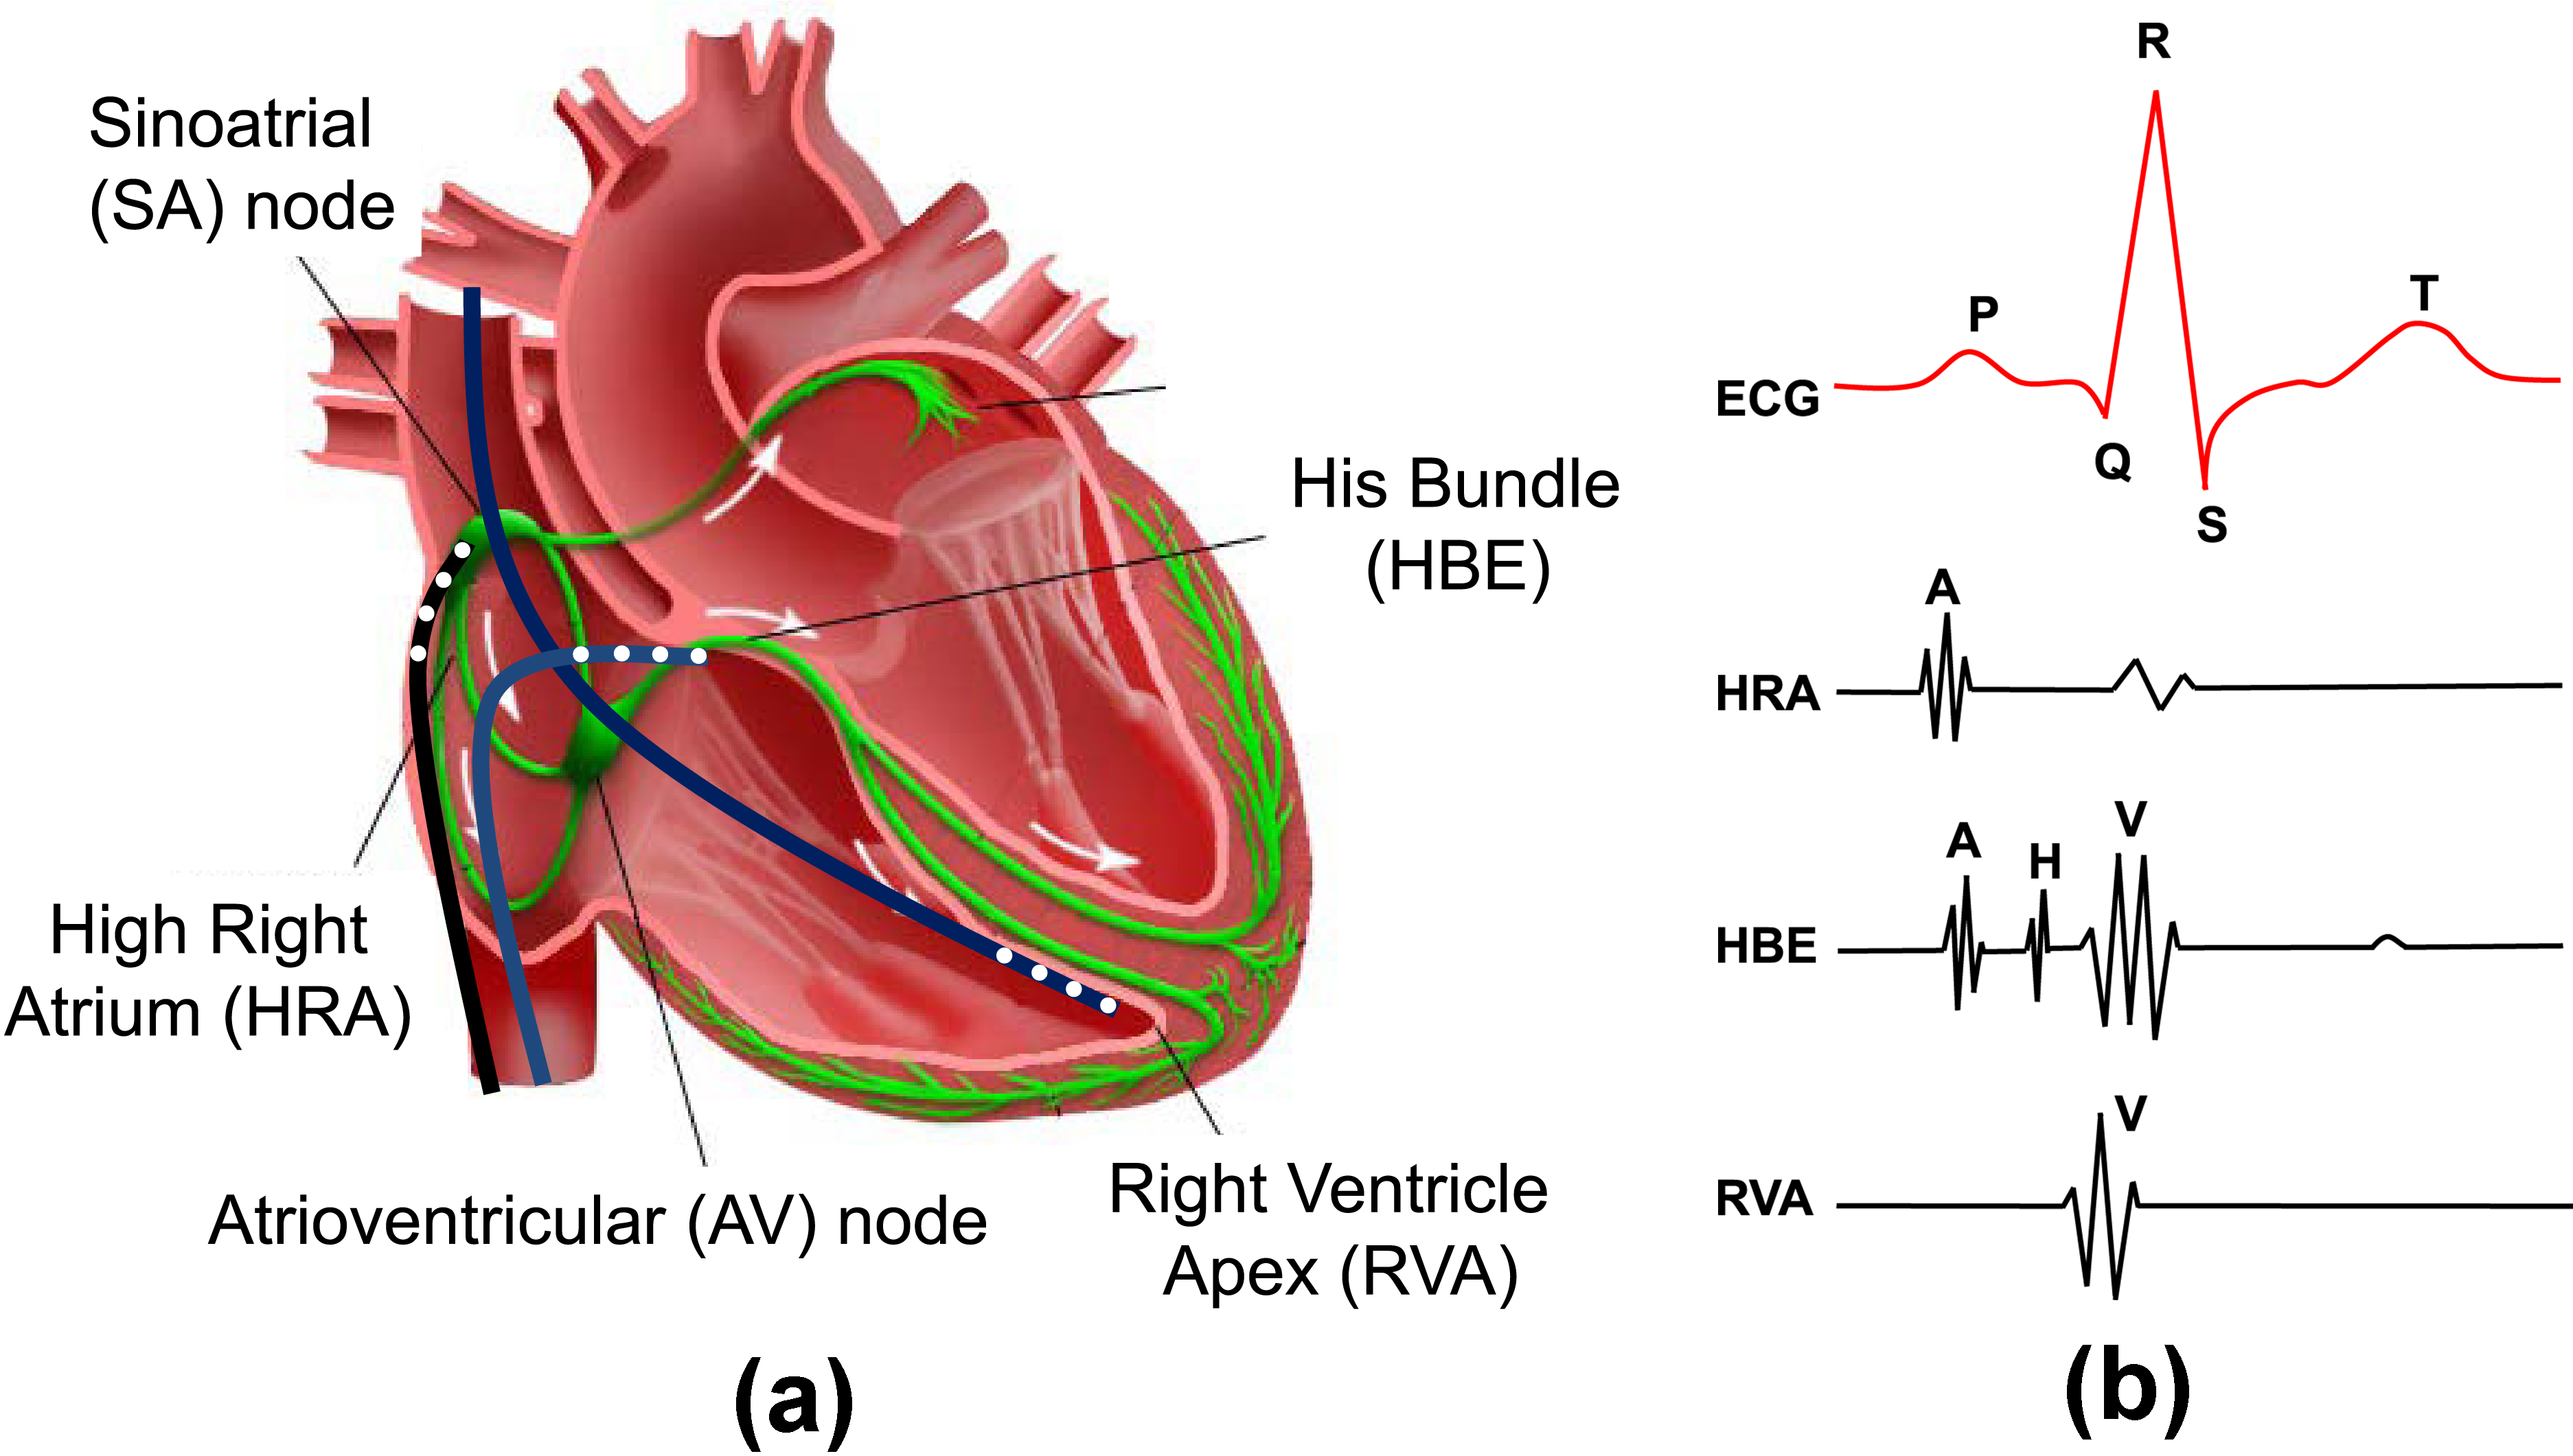
\includegraphics[width=0.9  \textwidth]{figs/probes.png}
		
%\vspace{-10pt}
\caption{\small (a) Probe locations for a general EP testing procedure. (b) EGM signals measured from the probes}
\label{fig:egm}
%\vspace{-15pt}
\end{figure} 

During an EP testing procedure, the physician place catheters inside the patient's heart to observe local electrical activities from different locations of the heart. The His bundle catheter (HBE) is particularly important when evaluating the atria-to-ventricle conduction path (\figref{egm}). For each A to V conduction there are 3 impulses which correspond to atrial contraction (A), His bundle activation (H) and ventricular activation (V).  In this case study, two pacing signals $a1$ and $a2$ are delivered to the heart from the HRA catheter. By gradually decreasing the pacing interval in each test, certain tissue along the A-V conduction path will be activated during its refractory period, thus affecting the conduction delay further down the conduction path and change the intervals between the impulses. \figref{book_1}.a shows the relation between pacing interval ($a1$-$a2$) and corresponding intervals between A, H and V impulses. On the left side it shows that interval $H_1-H_2$ and $V_1-V_2$ decrease but remain equal as the pacing interval decreases, indicating the tissue with the longest refractory period along the path is not between the His Bundle and the ventricles. When the pacing interval decreases to 350ms both intervals increases, indicating that the RRP of certain tissue has been reached and the tissue is between the atria and the His bundle. On the right it shows that the $A_2-H_2$ interval increases as the pacing interval decreases, which further proves the hypothesis that the AV node, which is between the atria and the His bundle has the longest refractory period along the A-V conduction path. We configured our heart model such that the AV node has the longest refractory period and performed the same study by decreasing the pacing interval. The result shows the exact same trend as the real patient (\figref{type_1}).
\begin{figure*}[!t]
\centering
		\subfigure 	[\small] 
		{
		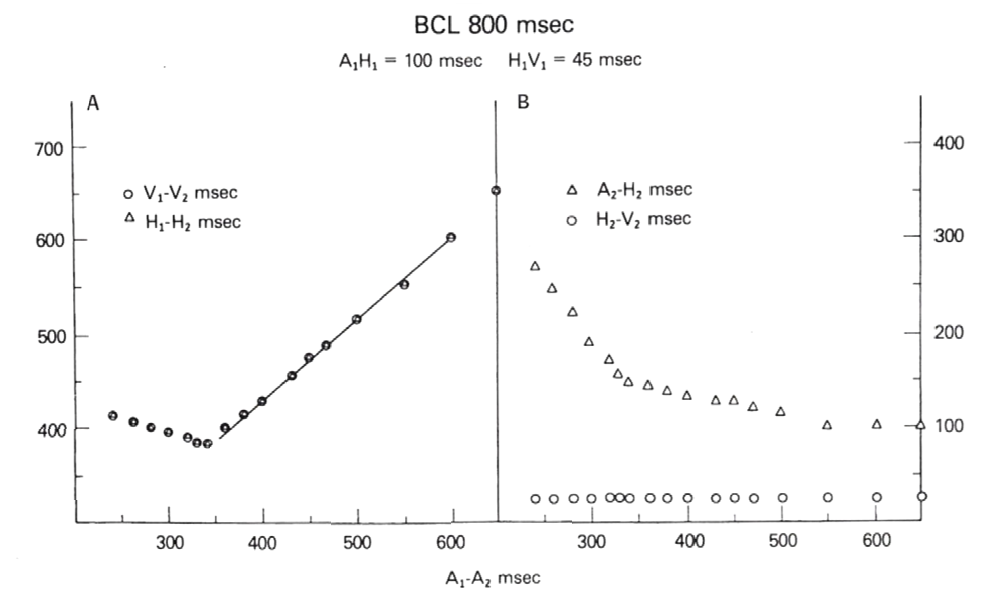
\includegraphics[width=0.5\textwidth]{figs/book_1.png}
		\label{fig:book_1}
		} 
		\subfigure [\small ] 
		{	
			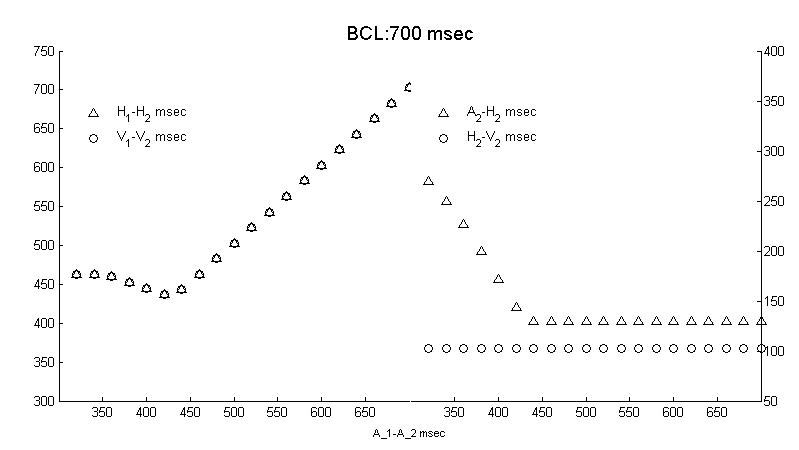
\includegraphics[width=0.45\textwidth]{figs/type_1.png} 
			\label{fig:type_1}
		}
\label{fig:Case_1}
%\vspace{-5pt}
\caption{\small Key interval values when the coupling interval shortens for (a) a real patient (\cite{josephson}) and (b) in heart model simulation (\cite{vhm_ecrts10}).}
%\vspace{-15pt}
\end{figure*} 


% \begin{figure}[\b]
% 	\center
% 	\vspace{-20pt}
% %	\includegraphics[width=0.49\textwidth]{figs/AV_reentry_circuit.pdf}
% 	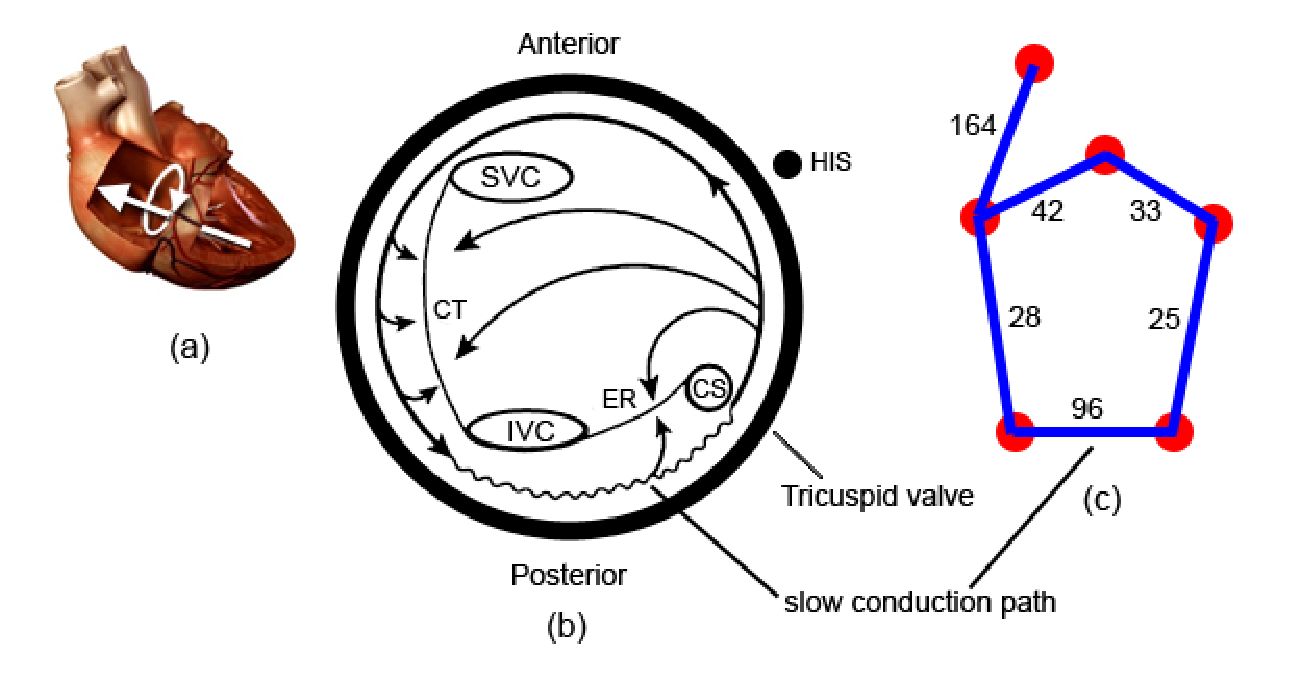
\includegraphics[width=0.5\textwidth]{figs/AFL_circuit.pdf}
% 	\center
% 	\vspace{-15pt}
% 	\caption{(a) The straight arrow shows the view of the AFL circuit from the right ventricle through the tricuspid valve into the right atrium, while the curved area shows the direction of conduction. (b) The circuit is bounded by the eustachian ridge (ER), connecting the  inferior vena cava (IVC) and the coronary sinus (CS), as well as the crista terminalis (CT), connecting the superior vena cava (SVC) and the IVC. The wavy line shows slow conduction through the CTI, bounded by the ER and the tricuspid valve (\emph{Adapted from} \cite{AFL_diag}). (c) The AFL circuit in the VHM extrapolates nodes and paths from the true physiology. The numbers show the values of conduction timers in the paths, with corresponding slow conduction path on the bottom.}
% 	\label{fig:AFL}
% \end{figure}

\subsection{Validating Models for Closed-loop Model Checking}
In model checking, a lot of complex dynamics of the environment are abstracted so that the environment model covers large number of environmental behaviors using non-determinism. The validity of the model is obtained by a valid initial model and a rigorous abstraction processes. In \cite{STTT13}, we started with a valid detailed deterministic model (as described above) and by applying different abstraction steps we were able to generate a series of non-deterministic heart models. Between each abstraction step, the heart models satisfy a timed simulation relationship (\cite{simulation}) which is described below. The timed simulation guarantees all behaviors are covered in the mode abstract model.

For two timed automata $T^1=\left\langle S^1,S_0^1,\Sigma^1,X^1,inv^1,E^1\right\rangle$ and $T^2=\left\langle S^2,S_0^2,\Sigma^2,X^2,inv^2,E^2\right\rangle$, a timed simulation relation is a binary relation $\textsf{sim}\subseteq \Omega^1\times \Omega^2$ where $\Omega^1$ and $\Omega^2$ are sets of states of $T^1$ and $T^2$. We say $T^2$ \textsf{time simulates} $T^1$ ($T^1 \preceq_t T^2$) if the following conditions holds:
\begin{itemize}
	\item Initial states correspondence: $(\left\langle s_0^1,\textbf{0}\right\rangle,\left\langle s_0^2,\textbf{0}\right\rangle)\in \textsf{sim}$
	\item Timed transition: For every $(\left\langle s_1,v_1\right\rangle,\left\langle s_2,v_2\right\rangle)\in\textsf{sim}$, if $\left\langle s_1,v_1\right\rangle\xrightarrow{\delta}\left\langle s_1,v_1+\delta\right\rangle$, there exists $\left\langle s_2,v_2+\delta\right\rangle$ such that $\left\langle s_2,v_2\right\rangle\xrightarrow{\delta}\left\langle s_2,v_2+\delta\right\rangle$ and \\$(\left\langle s_1,v_1+\delta\right\rangle,\left\langle s_2,v_2+\delta\right\rangle)\in\textsf{sim}$.
	\item Discrete transition: For every $(\left\langle s_1,v_1\right\rangle,\left\langle s_2,v_2\right\rangle)\in\textsf{sim}$, if $\left\langle s_1,v_1\right\rangle\xrightarrow{\sigma}\left\langle s_1',v_1'\right\rangle$, there exists $\left\langle s_2',v_2'\right\rangle$ such that $\left\langle s_2,v_2\right\rangle\xrightarrow{\sigma}\left\langle s_2',v_2'\right\rangle$ and $(\left\langle s_1',v_1'\right\rangle,\left\langle s_2',v_2'\right\rangle)\in\textsf{sim}$.
\end{itemize}


 

\chapter{Physiological Requirements}

Physiological requirements for medical devices specify the closed-loop conditions that the device is designed to achieve with its outputs to the patient. Unlike \emph{specifications} which specify desired device actions in response to the inputs from the patients, physiological requirements focus on the conditions of the patient with and without the device, which would indicate whether the device has fulfilled its intended goals. In this chapter, we address the following questions:
\begin{itemize}
	\vspace{-5pt}
	\item How requirements are different from specifications?
	\vspace{-5pt}
 	\item How can the requirements be represented?
	\vspace{-5pt}
	\item Are all requirements equally important?
\end{itemize}

% \begin{itemize}
% 	\item In contrast to specifications
%     \item Specified on physiological conditions during closed-loop interaction between the patient and the device.
%     \item Timing requirements
%     \item Monitor construction
% \end{itemize}

The most basic requirement for a pacemaker is to maintain the ventricular rate above a minimum level. The corresponding physiological requirement is:
\noindent
 \emph{The interval between two ventricular contractions should always be less or equal to 1000ms.} 

Note that this requirement focuses only on the condition of the patient (ventricular contractions), and there is no mention of the operation of the pacemaker or how the pacemaker should achieve the requirement. Here $1000ms$ is a patient-specific parameter. An example specification of a single chamber pacemaker corresponding to the requirement is:  
\noindent
\emph{If there is no sensed ventricular event 1000ms since the last ventricular event (sensed or paced), the pacemaker should deliver ventricular pacing.}
 
The specification is described using the terminology internal to the pacemaker software (paced and sensed events), and specifies the action of the pacemaker corresponding to certain inputs. For more complex requirements, multiple specifications have to work together to achieve the requirement. Therefore there may exist executions that satisfy all the specifications but not the corresponding requirement. Verifying physiological requirements requires knowledge of the physiological condition and how device interacts with the physiological environment, thus can only be performed in closed-loop. 

Devices are designed to improve certain physiological conditions, the performance of the devices is evaluated on the difference between the patient conditions without the device and with the device. The device should also avoid deteriorating certain patient conditions, thus physiological requirements are specified in the form of:
$$C_{pre}\rightarrow C_{post}$$
in which $C_{pre}$ is the physiological conditions without the device,  and $C_{post}$ is the physiological condition with the device. For model-based closed-loop verification, $C_{pre}$ is often in form of a set of constraints on patient parameters. As a special case, $C_{pre}$ can equal to $true$, means that $C_{post}$ should be satisfied under all possible conditions.

One of the challenges for developing medical device software is to convert physiological requirements, which are generally informal descriptions of physiological conditions, into mathematical descriptions that can be used by verification tools.  In model-based verification, these physiological conditions are mapped onto constraints on model parameters. %In the following section, we use the heart model as example to show this process.

While the device is to aid the physiological function under certain conditions, it must deal with all possible environment conditions. However, in certain extreme conditions, not all physiological requirements can be satisfied due to the limitations of device function. It is thus intuitive to assign priorities to the requirements and assess the capability of the device to prioritize more important requirements in these scenarios. 

We use pacemaker as example to demonstrate how to convert physiological descriptions into mathematical requirements and how priorities of the requirements affect the verification process.

%For convenience, requirements are usually specified with binary results (satisfied/unsatisfied). quantitative
\noindent
\textbf{1. Encoding Physiological Conditions:}  \figref{state} lists example heart conditions and their corresponding constraints on heart model parameters.
\begin{figure}[!t]
	\center
	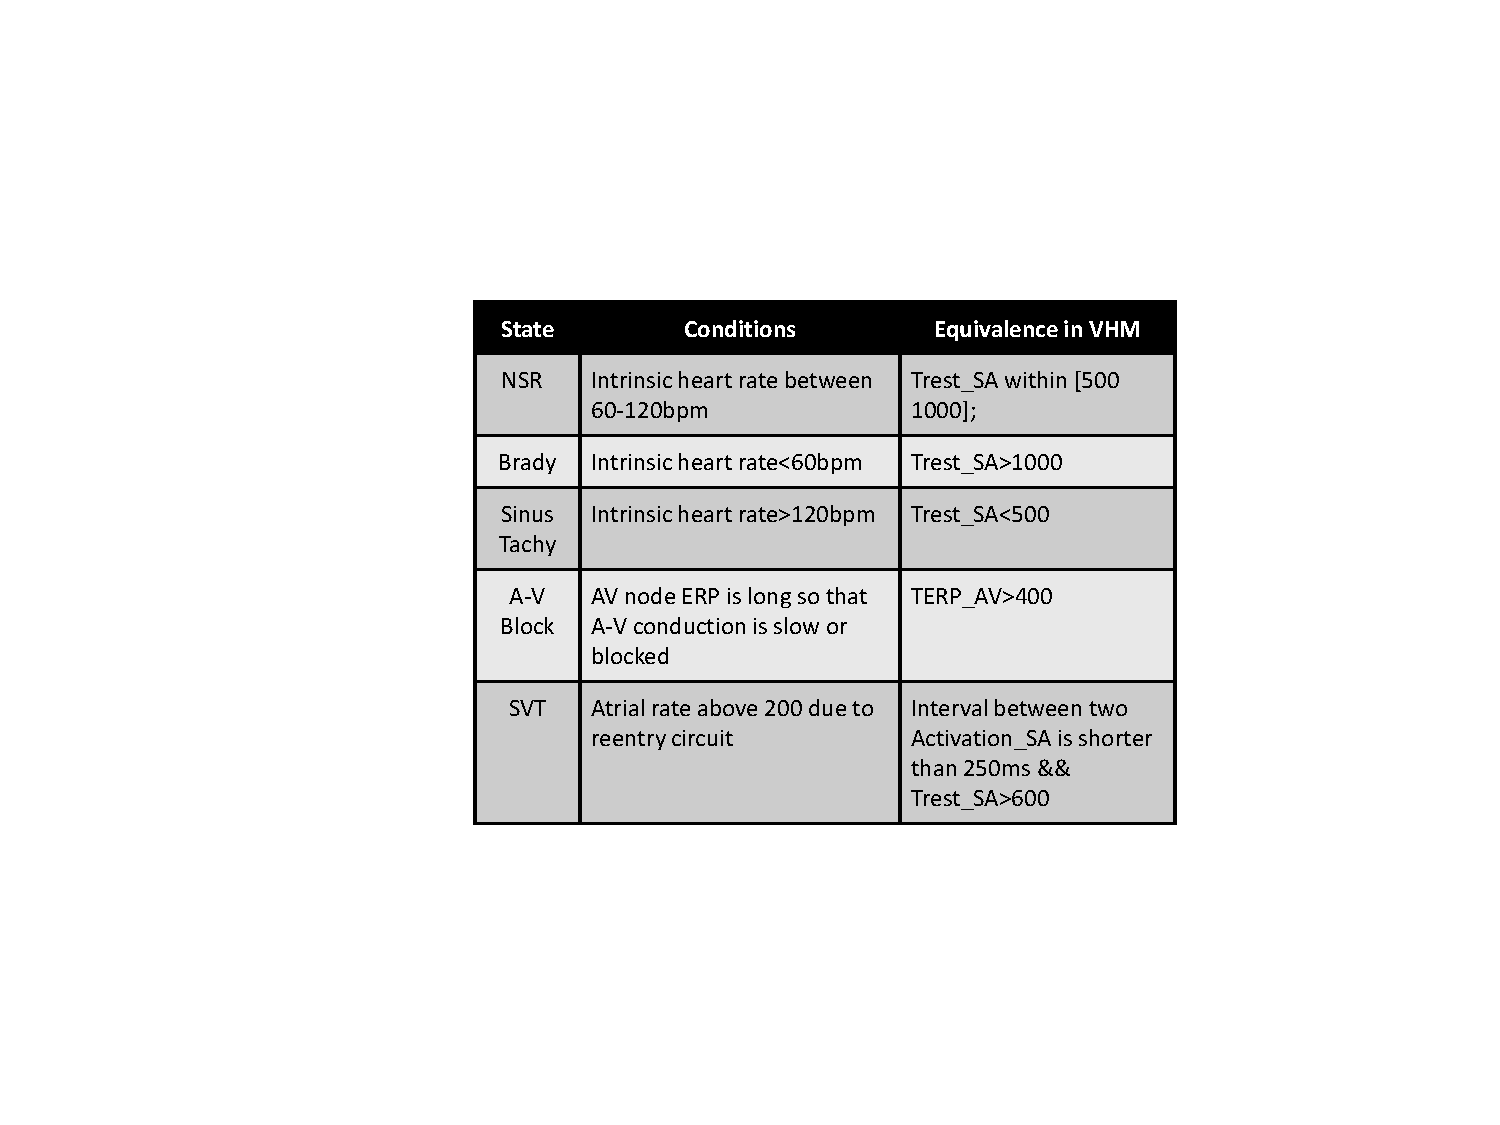
\includegraphics[width=0.70\textwidth]{figs/state.pdf}
	\center
	\vspace{-10pt}	
	\caption{Patient state and equivalence in the heart model}
	\vspace{-10pt}	
	\label{fig:state}
\end{figure}
\noindent
\\\textbf{2. Conditional Requirements:} Physiological requirements are in general conditional requirements. Specifying conditional requirements enables tighter constraints on the closed-loop system. \figref{conditional} shows a list of conditional requirements for normal sinus rhythm (NSR), supraventricular tachycardia (SVT), and bradycardia used during the pacemaker case study. 
\begin{figure}
	\center
	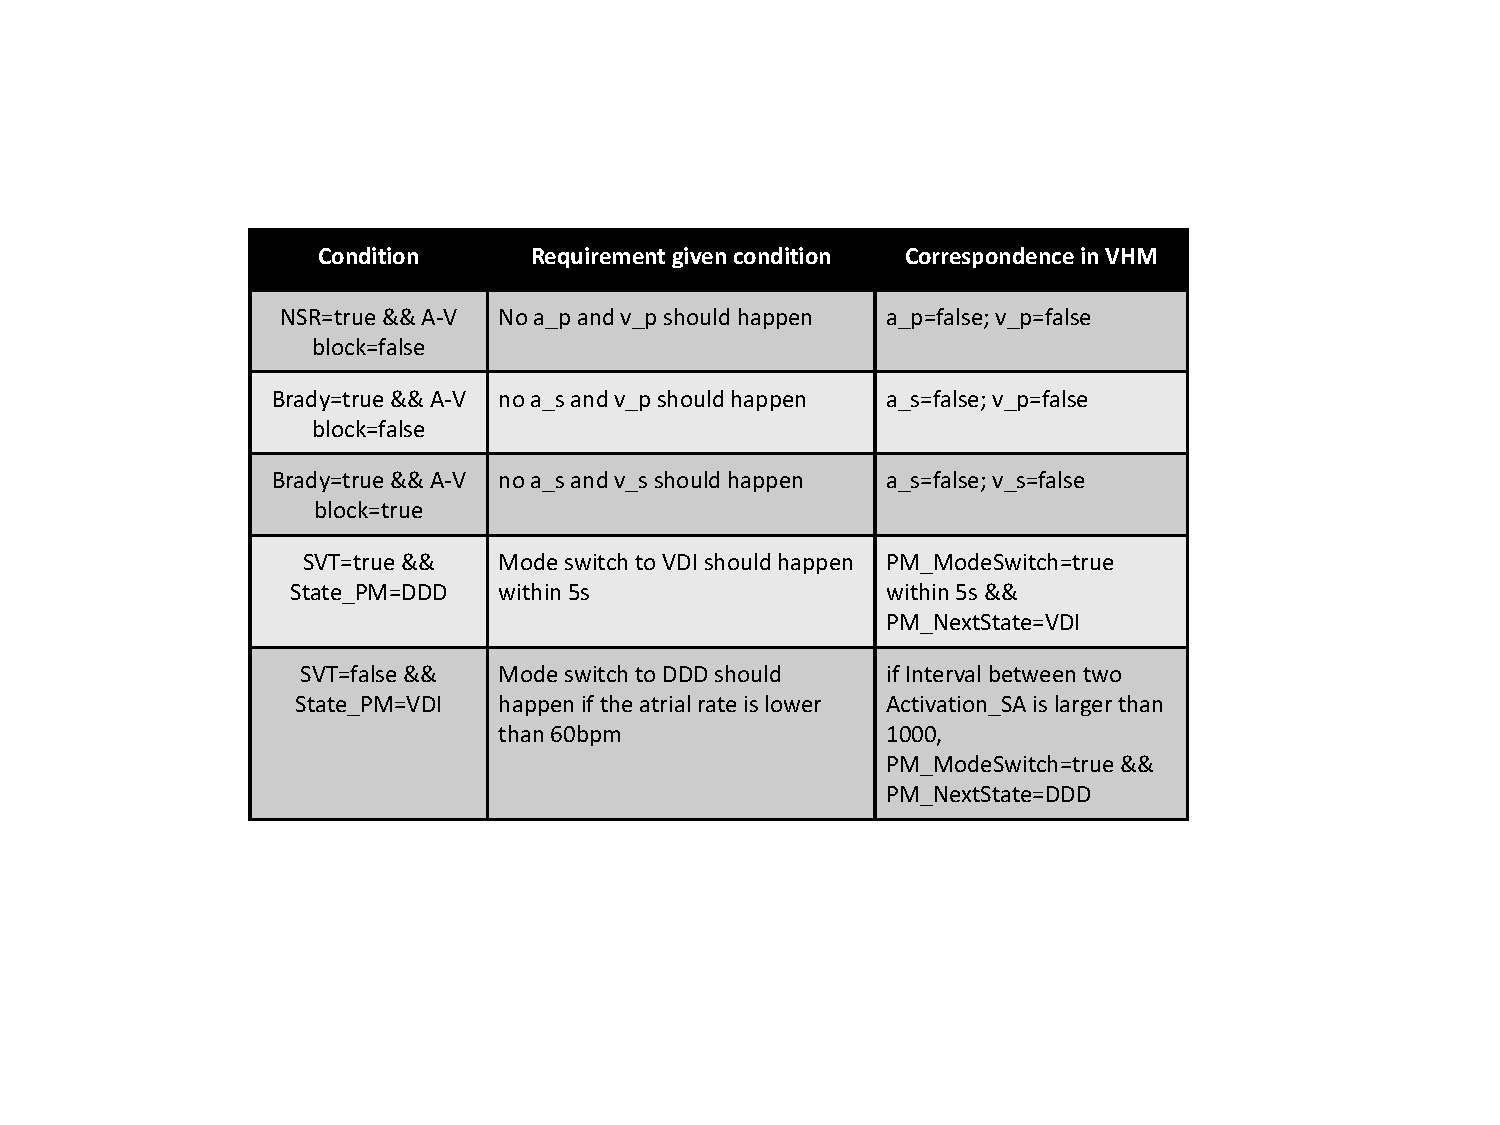
\includegraphics[width=0.7\textwidth]{figs/conditional.pdf}
	\center
	\vspace{-10pt}
	\caption{Conditional requirements for the close-loop system}
		%\vspace{-15pt}
	\label{fig:conditional}
\end{figure}
\begin{figure}
	\center
	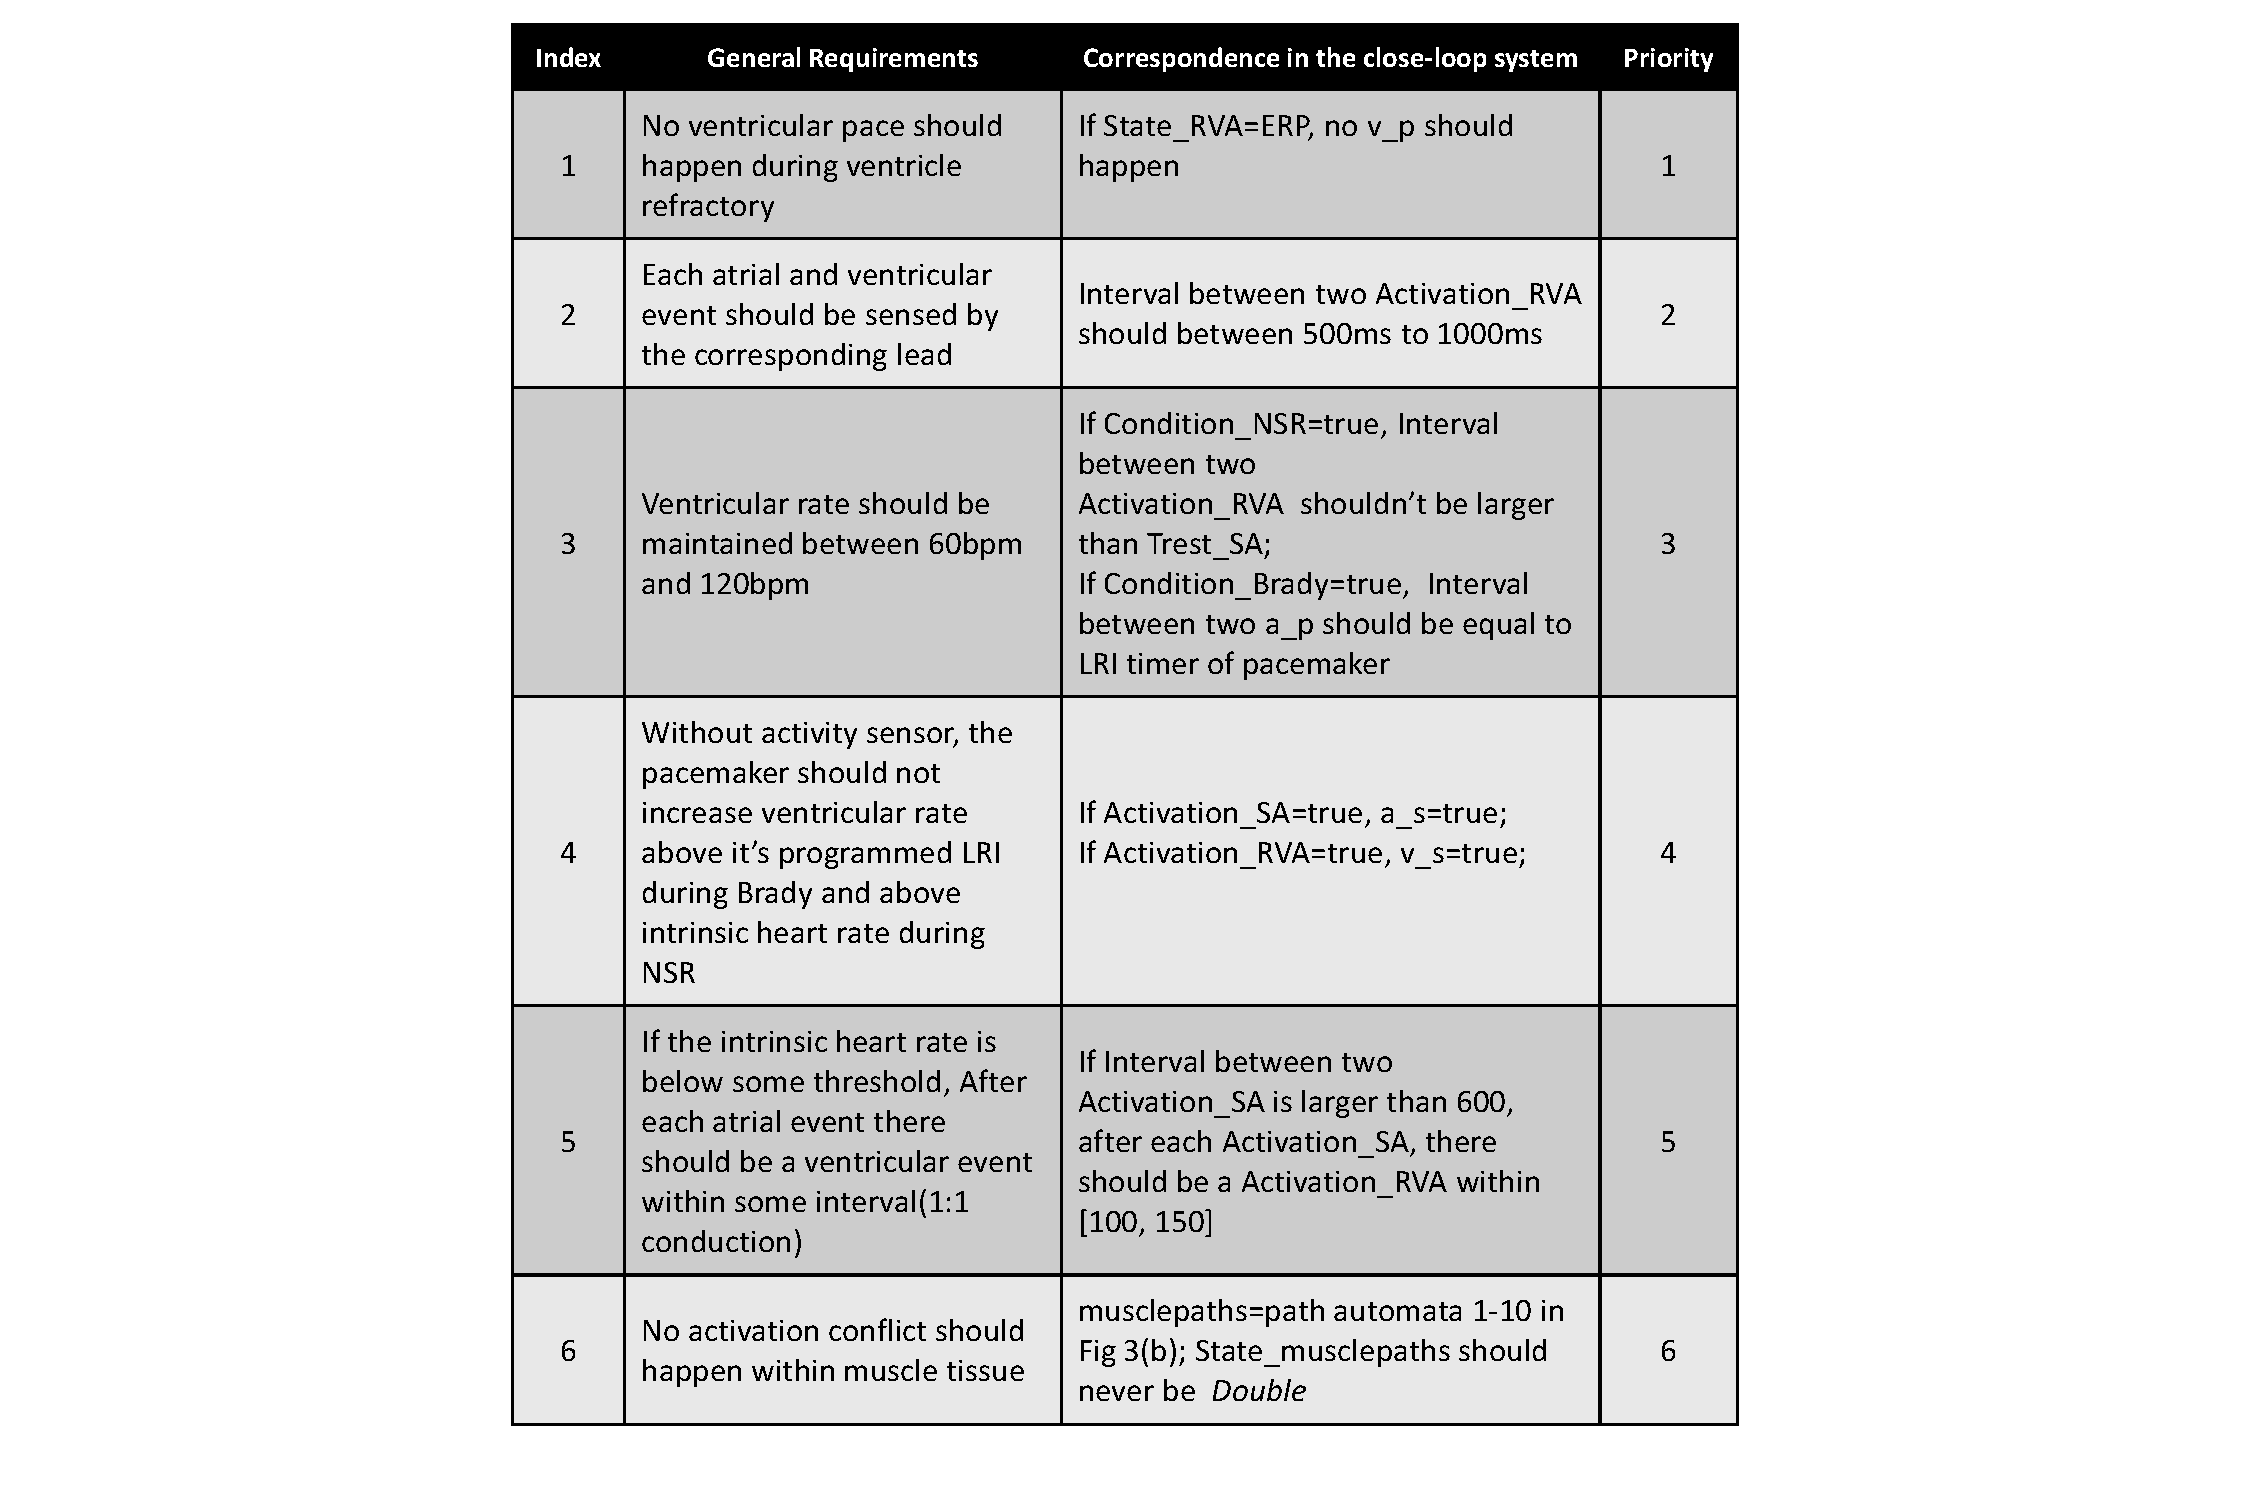
\includegraphics[width=0.7\textwidth]{figs/properties.pdf}
	\center
	\vspace{-10pt}
	\caption{General requirements for the close-loop system}
		%\vspace{-15pt}
	\label{fig:properties}
\end{figure}
\noindent
\\\textbf{3. Requirement Hierarchy}
For a closed-loop system including a heart $H$ and a pacemaker $P$: $S=H || P$ and two requirements $\varphi_1$ and $\varphi_2$ such that $\mathbb{P}_{\varphi_1}<\mathbb{P}_{\varphi_2}$, the following statement should always hold:
\vspace{-5pt}
$$H\models\varphi_2\rightarrow H||P\models\varphi_2$$
\noindent
meaning if a higher priority requirement is satisfied by the open-loop environment, it should be satisfied by the closed-loop system as well. An example violation of the statement is:
$$H\not\models\varphi_1 \&\& H\models\varphi_2 \&\& H||P\models\varphi_1 \&\& H||P\not\models\varphi_2$$
\noindent
which should not be allowed. In our closed-loop verification of pacemaker, the list of physiological requirements with assigned priorities are showing in \figref{properties}.




%\section{Requirement Representations}
%\subsection{TCTL}
%\subsection{Simulink Block}



\chapter{A Dual Chamber Pacemaker Specification}

As part of the model-based design, it is important to have a functional and formal model of the device software for testing and formal verification respectively. In our study, we focus on the implantable  pacemaker since it is one of the simpler implantable cardiac devices as its functionality is based only on timing and does not consider signal morphology. This serves as a good base case to demonstrate the proposed methodology.  In this chapter we describe the basic specification and formal implementation of a dual chamber pacemaker, as well as a more advanced function on mode switching. The specifications are based on the algorithm descriptions in \cite{compass} and the functional description released as part of the Pacemaker Challenge (\cite{challenge}). 
We aim to answer the following questions here:
\begin{itemize}
	\vspace{-5pt}
	\item How are the pacemaker's timers specified to maintain the appropriate heart rhythm?
	\vspace{-5pt}
   	\item What happens if new functionality are applied to the basic model?
\end{itemize}

The artificial pacemaker is designed for patients with bradycardia (i.e. slow heart rate). Two leads, one in the right atrium and one in the right ventricle, are inserted into the heart and fixed onto the inner wall of the heart. These two leads monitors the local activation of the atria and the ventricles, and generate corresponding sensed events (AS, VS) to its software. The software determines the heart condition by measuring time difference between events and delivers pacing events (AP, VP) to the analog circuit when necessary. The analog circuit then delivers pacing signals to the heart to maintain heart rate and A-V synchrony. In order to deal with different heart condition, pacemakers are able to operate in different modes. The modes are labeled using a three character system (e.g. $xyz$). The first position describes the pacing locations, the second location describes the sensing locations, and the third position describes how the pacemaker software responds to sensing. Here we introduce the widely used DDD mode pacemaker which is a dual chamber mode with sensing and pacing in both atrium and ventricle. 

\begin{figure}[!t]
\center
%\vspace{-10pt}
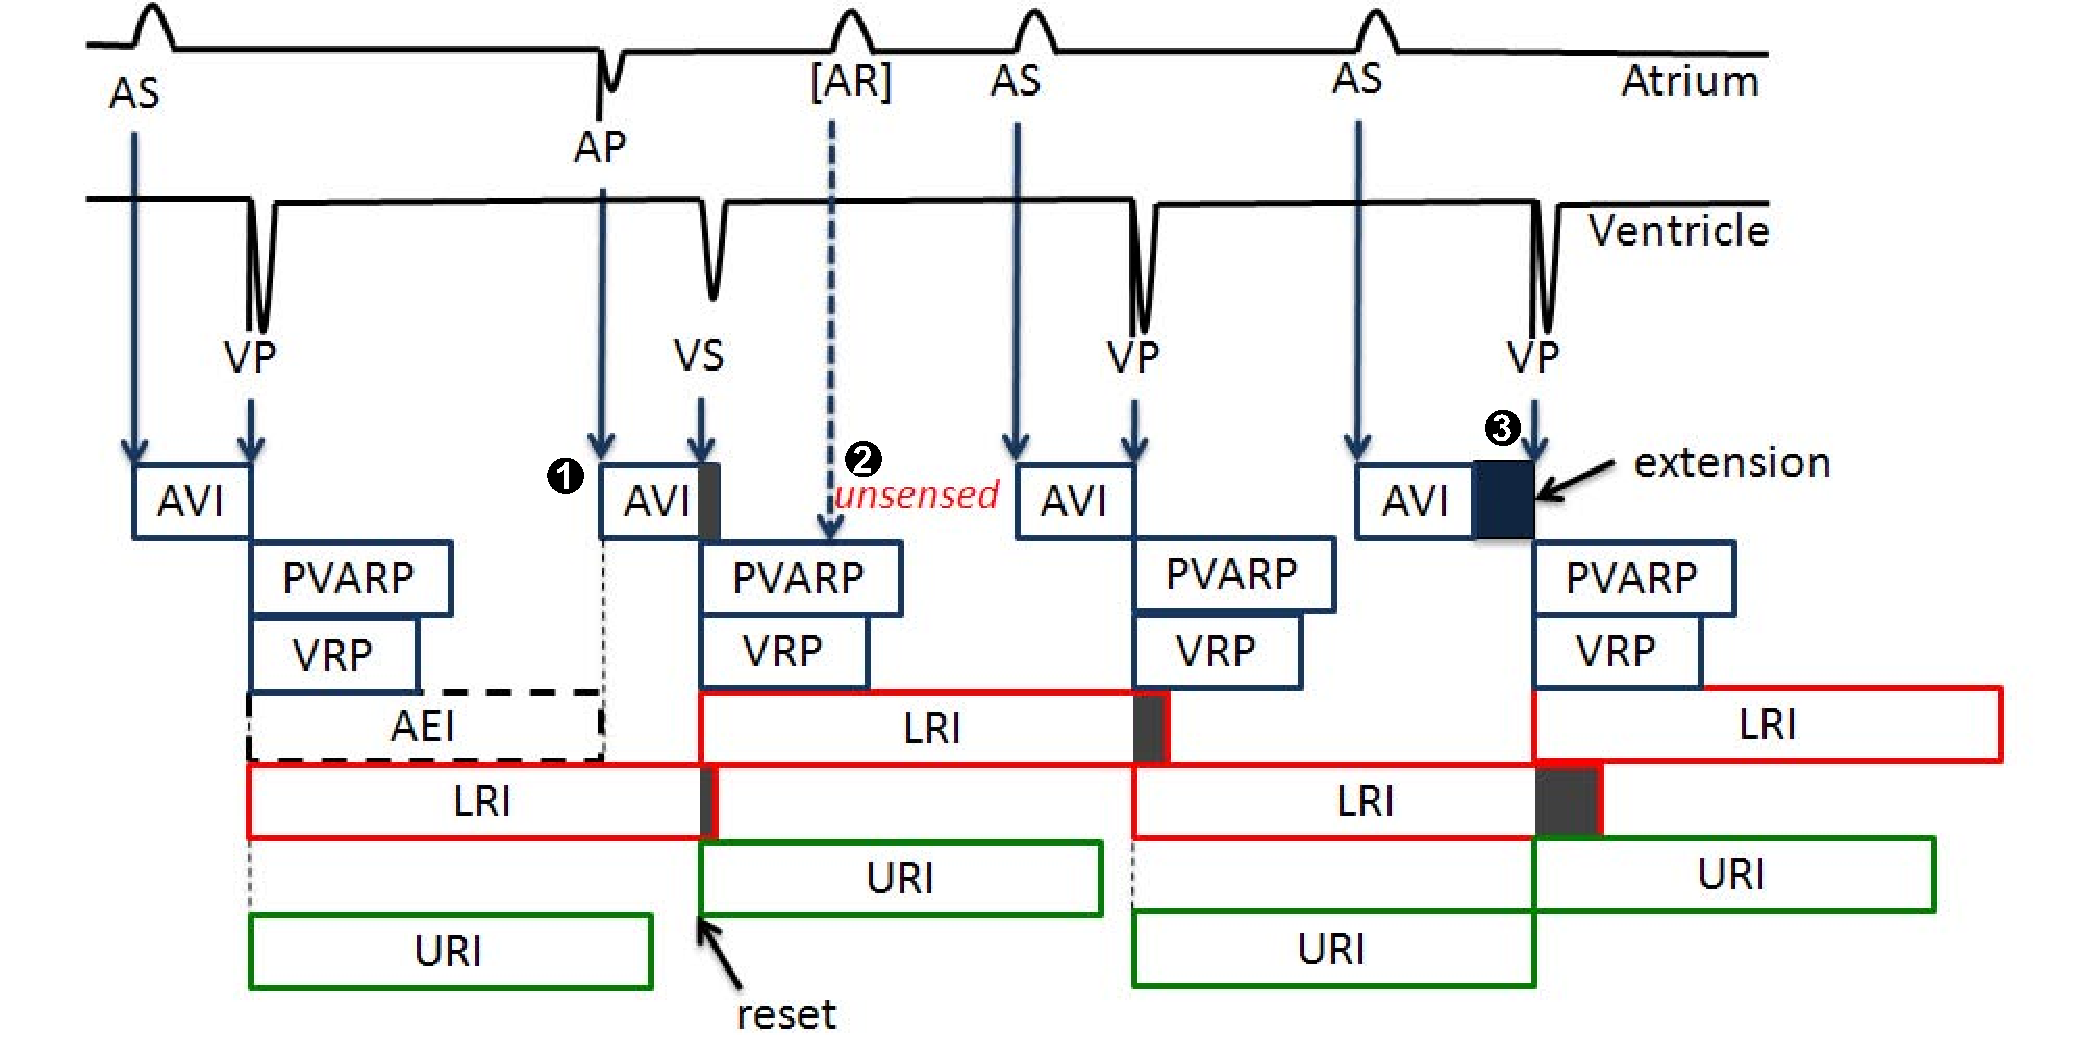
\includegraphics[width=0.7\textwidth]{figs/PM_timers.pdf}
%\vspace{-10pt}
\caption{Basic 5 timing cycles for a dual chamber pacemaker}
\label{fig:PMtimers}
%\vspace{-10pt}t

\end{figure} 
\section{Basic Specifications of a DDD Pacemaker}
The DDD pacemaker has five basic timing cycles triggered by external and internal events, as shown in \figref{PMtimers}. We decomposed our pacemaker model into five components which correspond to the five timers. $P=LRI\| AVI\| URI\| PVARP\| VRP$. These components synchronize with each other using broadcast channels and shared variables (as shown in \figref{PMdesign}). 

\subsection{Lower Rate Interval (LRI)}
%\vspace{-5pt}
The Lower Rate Interval (LRI) component is shown in \figref{PMdesign}(a). This component defines the longest interval allowed between two ventricular events, thus keeping the heart rate above a minimum value. In DDD mode, the LRI interval is divided into a V-A interval (TLRI-TAVI) and a A-V interval (TAVI). The LRI component maintains a maximum V-A delay while the AVI component maintains a maximum A-V delay so together they maintain the maximum V-V delay. In the LRI component, the clock is reset when a ventricular event \textsf{(VS, VP)} is received. If no atrial event has been sensed \textsf{(AS)}, the component will deliver atrial pacing \textsf{(AP)} after TLRI-TAVI. 

%\vspace{-5pt}
\subsection{Atrio-Ventricular Interval (AVI) and Upper Rate Interval (URI)}
%\vspace{-5pt}
The function of the AVI component defines the longest interval between an atrial event and a ventricular event. If there is no ventricular event \textsf{(VS)}  within TAVI after an atrial event \textsf{(AS, AP)}, and the time since the last ventricular event \textsf{(VS, VP)} is longer than TURI, the component will deliver ventricular pacing \textsf{(VP)}. The URI limits the ventricular pacing rate by enforcing a lower bound on the times between consecutive ventricle events. The UPPAAL design of AVI and URI component is shown in \figref{PMdesign}(b) and (c).%The UPPAAL design of AVI component is shown in 

%\vspace{-10pt}
\subsection{Post Ventricular Atrial Refractory Period (PVARP) and Post Ventricular Atrial Blanking (PVAB)}
%\vspace{-5pt}
Ventricular events, especially Ventricular Pace (VP) are sometimes so strong that the atrial lead can sense the activation as well. This signal may be falsely recognized as an atrial event and disrupt normal pacemaker function. This scenario is called crosstalk and was discussed in our previous work (~\cite{vhm_embc11}). In order to prevent this undesired behavior, and filter potential noises, there is a blanking period (PVAB) followed by a refractory period (PVARP) for the atrial events after each ventricular event \textsf{(VS, VP)}. Atrial events during PVAB are ignored and atrial events during PVARP trigger \textsf{AR!} events which can be used in some advanced diagnostic algorithms. The UPPAAL design of PVARP component is shown in \figref{PMdesign}(d).

%\vspace{-10pt}
\subsection{Ventricular Refractory Period (VRP)}
%\vspace{-5pt}
The VRP follows each ventricular event \textsf{(VP, VS)} to filter noise and early events in the ventricular channel which could otherwise cause undesired pacemaker behavior. \figref{PMdesign}(e) shows the UPPAAL design of VRP component.

\begin{figure}[!t]
\center
%\vspace{-10pt}
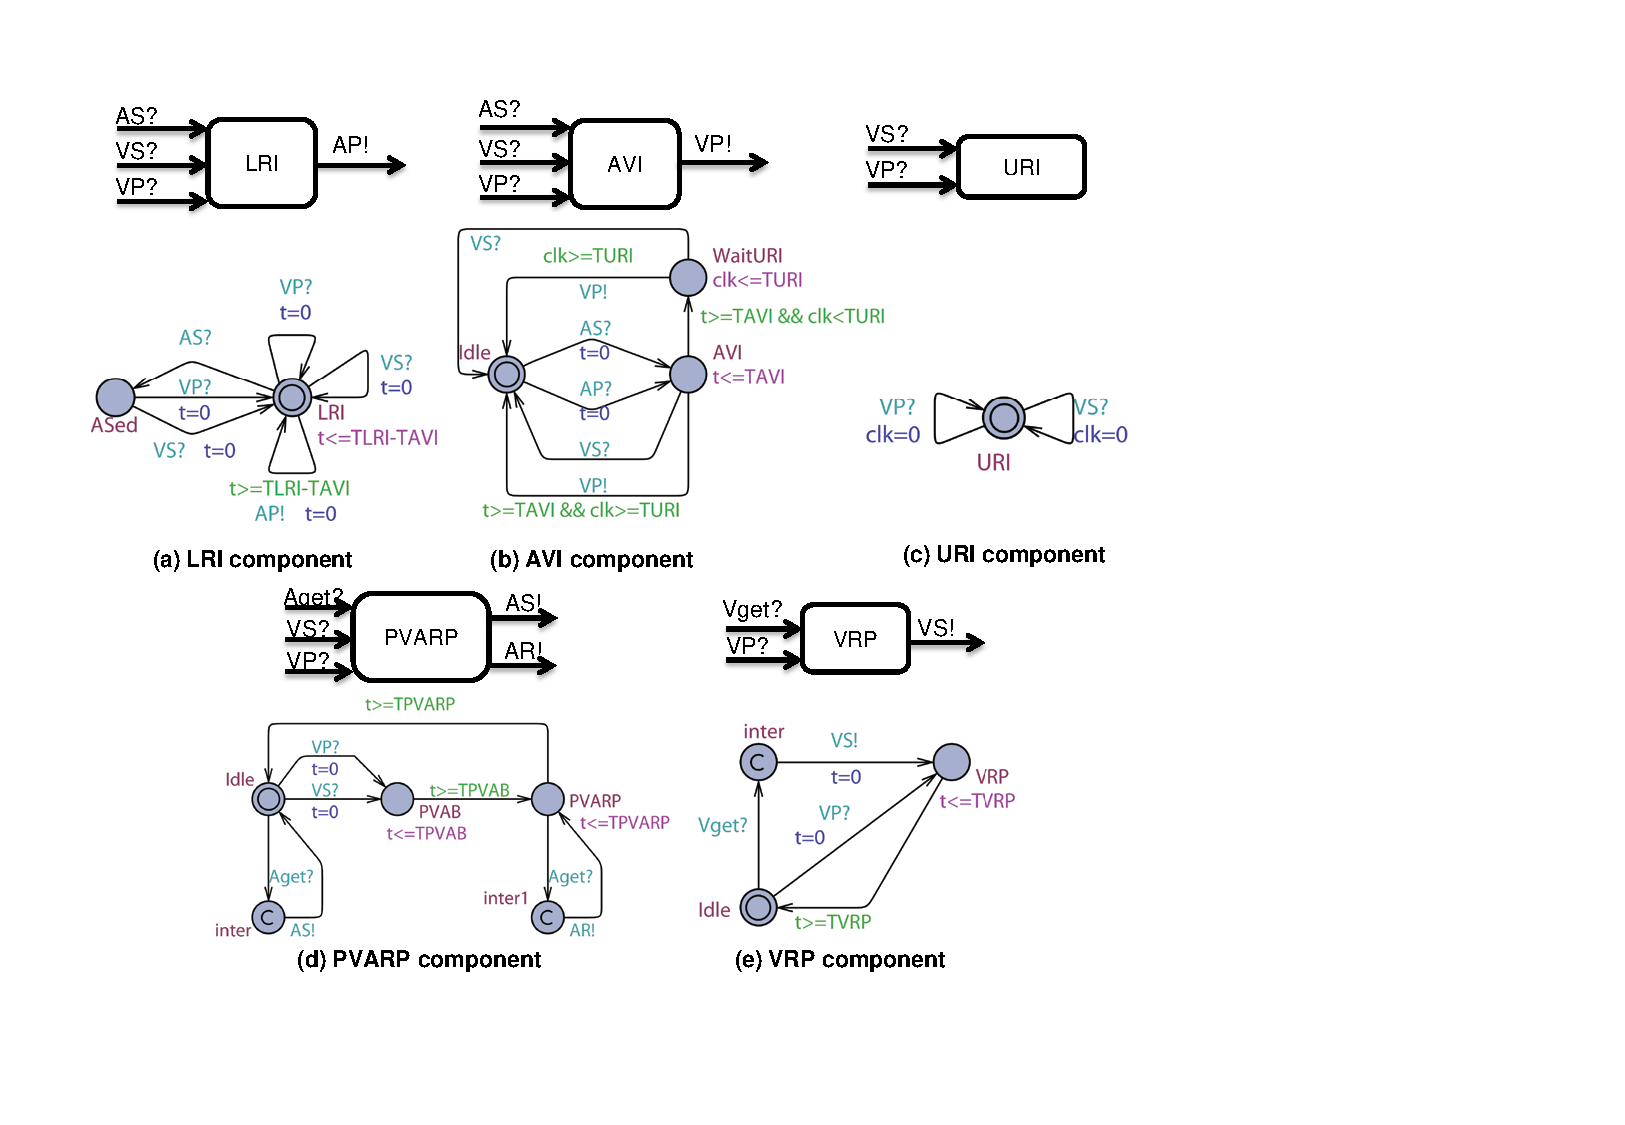
\includegraphics[width=0.9\textwidth]{figs/pacemaker.pdf}
%\vspace{-10pt}
\caption{Basic 5 timing cycles for a dual chamber pacemaker}
\label{fig:PMdesign}
%\vspace{-10pt}
\end{figure} 

\section{Mode Switch Operation: Atrial Tachycardia Response}
Supraventricular Tachycardia (SVT) is an arrhythmia with an abnormally fast atrial rate. %\figref{SVT} is a series of simulation results for closed-loop interaction between a heart model with SVT and the pacemaker model. The atrial and ventricular channels show electrogram inputs to the pacemaker and the pacemaker channel shows the corresponding events received and generated by the pacemaker software, \cite{vhm_embc11}.
Typically, in a heart without pacemaker, the AV node, which has a long refractory period, can filter most of the fast atrial activations during SVT, thus the ventricular rate remains relatively normal. \figref{SVT_none} demonstrates a pacemaker event trace during SVT, with a pacemaker in ODO mode, which just sensing in both channels. 
As there is no pacing in ODO mode, the heart is in open-loop with the pacemaker. In this particular case, every 3 atrial events (AS) correspond to 1 ventricular event (VS) during SVT. 
As an arrhythmia, SVT is still considered a safe heart condition since the ventricles operate under normal rate and still maintain adequate cardiac output. 

However, in the closed loop case with the DDD pacemaker, the AVI component of a dual chamber pacemaker is equivalent to a virtual pathway in parallel to the intrinsic conduction pathway between the atria and the ventricles. The pacemaker tries to maintain 1:1 A-V conduction and thus increases the ventricular rate inappropriately to match the atrial rate.  This is known as Pacemaker Mediated Tachycardia (PMT) as the heart would have been safe without the pacemaker and its virtual pathway. \figref{SVT_DDD} shows the pacemaker trace of the same SVT case with DDD pacemaker. Although half of the fast atrial events are filtered by the PVARP period ([AR]s), the DDD pacemaker still drives the closed-loop system into 2:1 A-V conduction with faster ventricular rate. Maintaining A-V delay is less important than maintaining an appropriate ventricular rate. The DDD pacemaker violates a higher priority requirement in order to satisfy a lower priority requirement, which is inappropriate.
\begin{figure*}[!t]
\centering
		\subfigure [\small]{			
		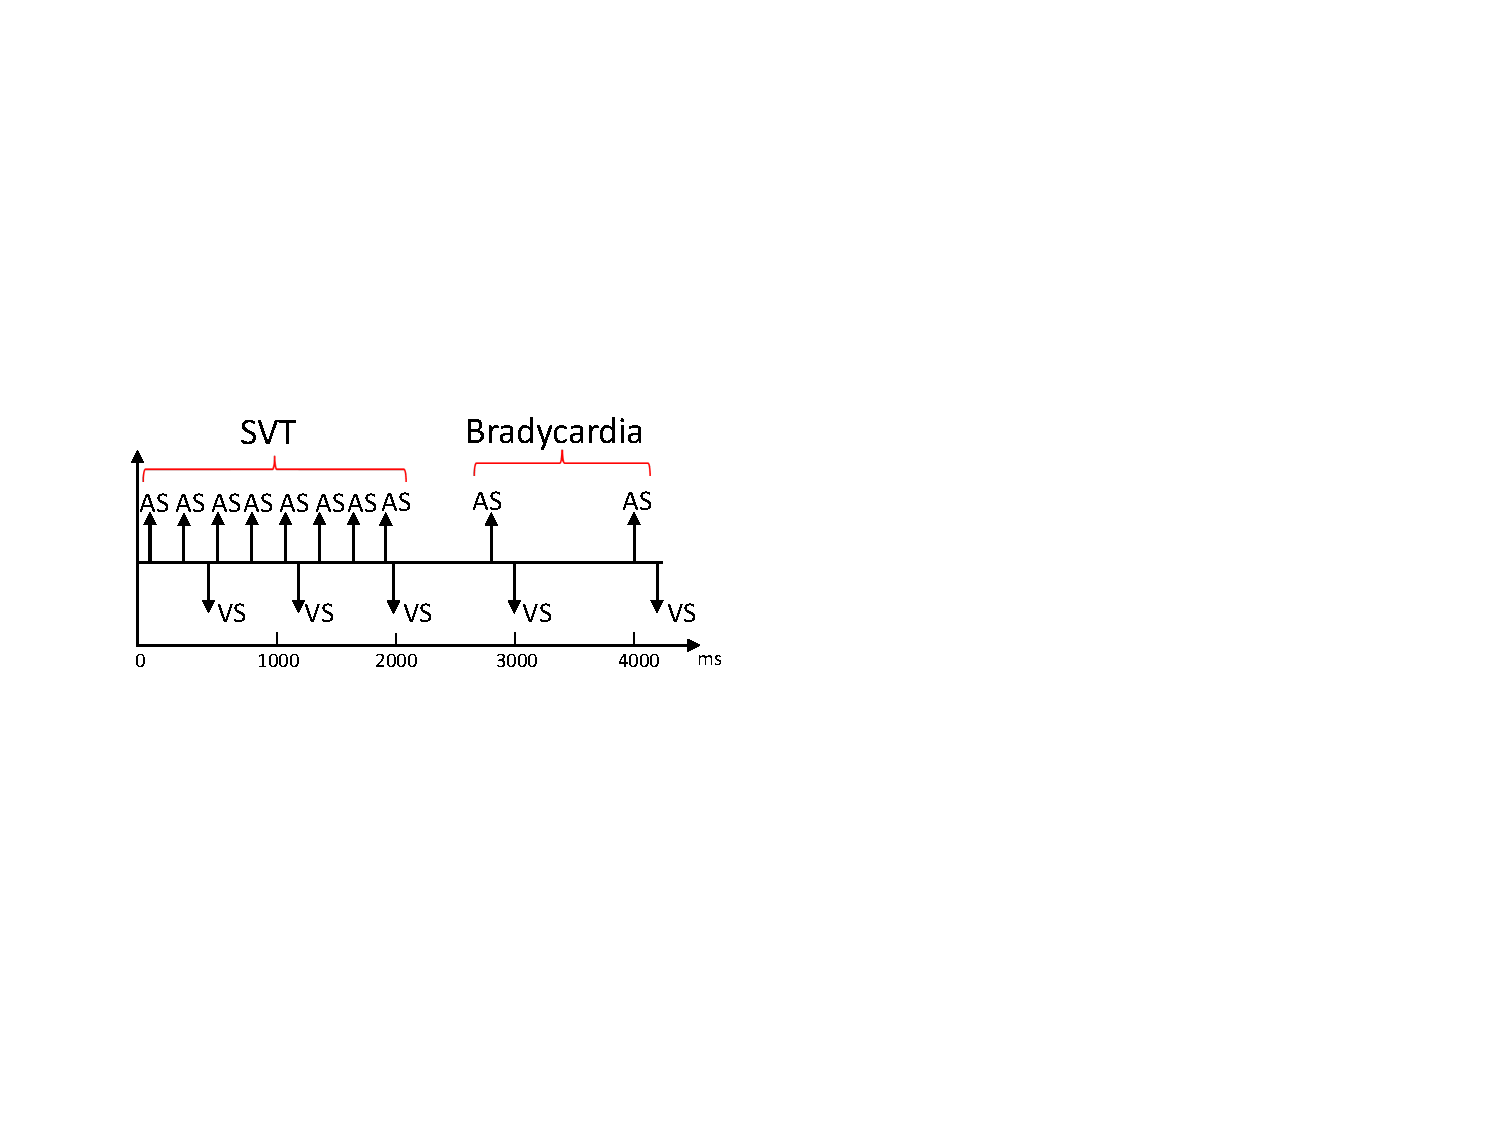
\includegraphics[width=0.5  \textwidth]{figs/SVT_none.pdf}
		\label{fig:SVT_none}
		} 
%	\hspace{.1in}%
\vspace{-10pt}
		
		\subfigure [\small] 
		{
		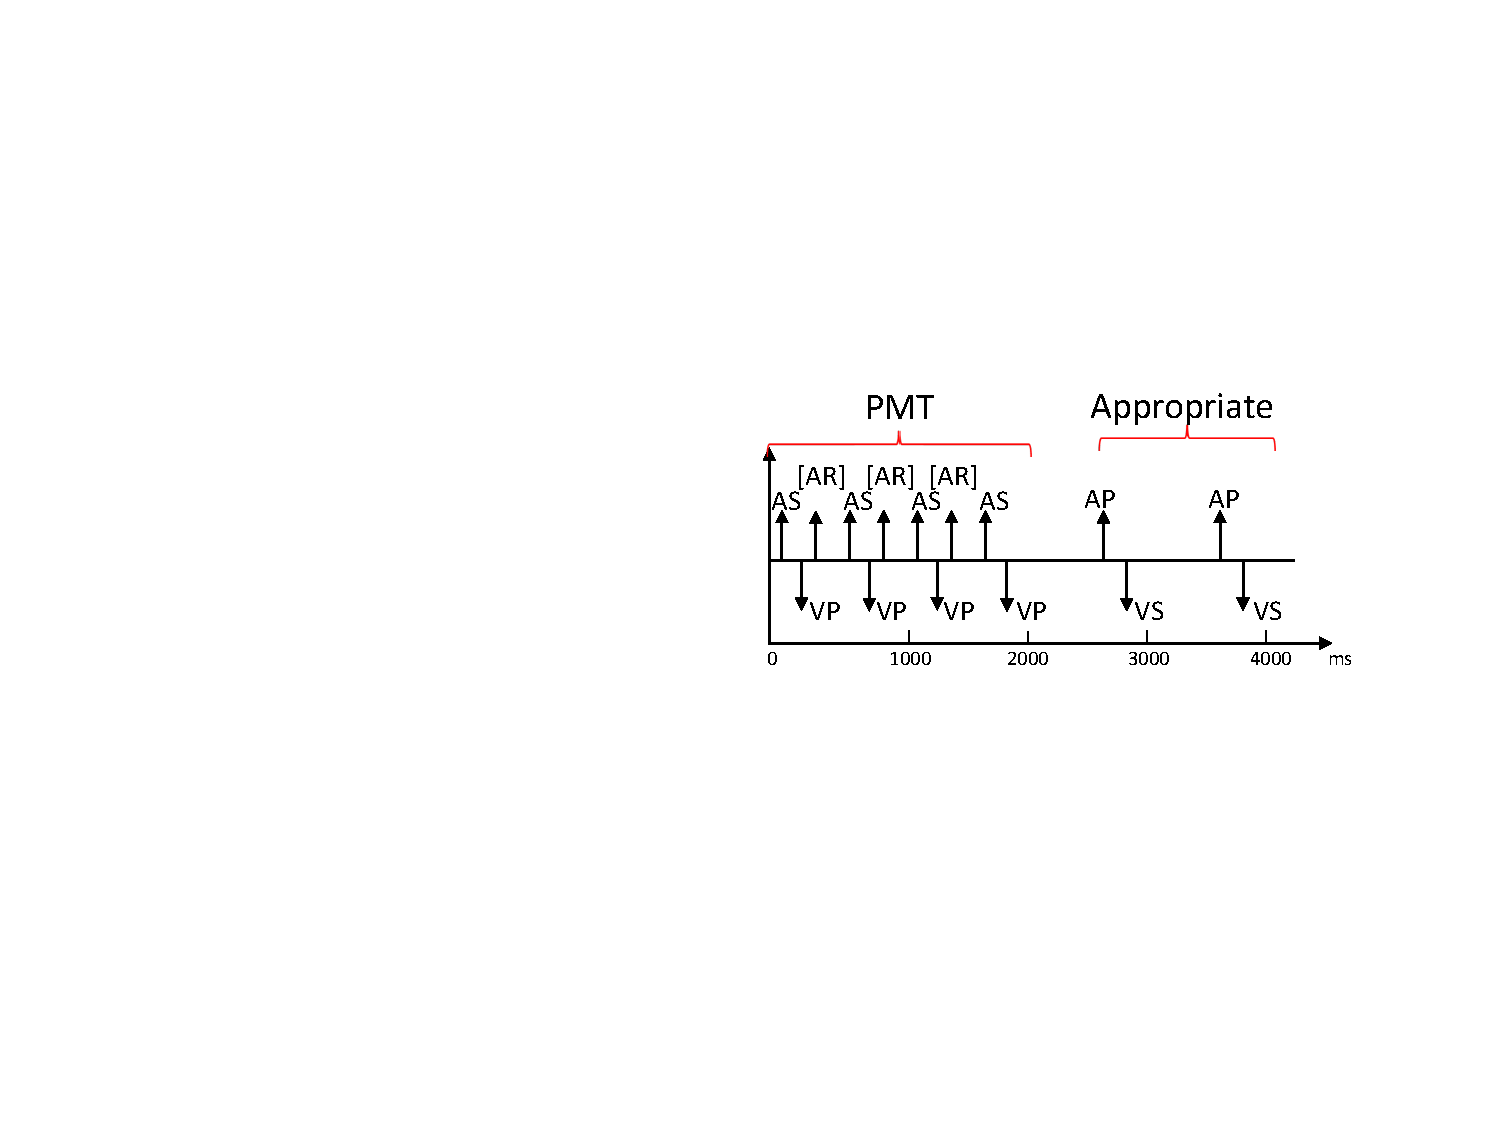
\includegraphics[width=0.5\textwidth]{figs/SVT_DDD.pdf}
		\label{fig:SVT_DDD}
		} 
\vspace{-10pt}
\caption{\small Benign open loop case: SVT with ODO pacemaker (b) Dangerous closed-loop-case SVT with DDD pacemaker}
%\vspace{-15pt}
\end{figure*} 

Pacemaker manufacturers have designed algorithms to detect and terminate these behaviors. Intuitively, the mode-switch algorithm first detects SVT. After confirmed detection, it switches the pacemaker from a dual-chamber mode to a single-chamber mode. During the single-chamber mode, the A-V synchrony function of the pacemaker is deactivated thus the ventricular rate is decoupled from the fast atrial rate. After the algorithm determines the end of SVT, it will switch the pacemaker back to the dual chamber mode. 

The mode-switch algorithm (also known as atrial tachycardia response) specification we use is similar to the one described in the Boston Scientific pacemakers' manual (\cite{compass}). The algorithm first measures the interval between atrial events outside the blanking period (AS, AR). The interval is considered as \emph{fast} if it is above a threshold (\emph{Trigger Rate}) and \emph{slow} otherwise. In our UPPAAL model we model it as $INT$ (see \figref{dur_count} (1)). A counter $CNT$ increments for \emph{fast} events and decrements for \emph{slow} events (see \figref{dur_count} (2)). After the counter value reaches the \emph{Entry Count}, the algorithm will start a \emph{Duration} ($DUR$) ,which is a time interval used to confirm the detection of SVT (see \figref{dur_count} (3)). In the \emph{Duration}, the counter keeps counting. If the counter value is still positive after the \emph{Duration}, the pacemaker will switch to the VDI mode (\emph{Fallback mode}). In the VDI mode, the pacemaker only senses and paces the ventricle. At any time if the counter reaches zero, the \emph{Duration} will terminate and the pacemaker is switched back to DDD mode.
% to show some interesting findings. The basic idea of this simplified model is explained in detail. \\
%\mySubSubSection{UPPAAL model for mode-switch algorithm}
In our UPPAAL model of the mode-switch algorithm, we use nominal parameter values from the clinical setting. We define \emph{trigger rate} at 170bpm (350ms), \emph{entry count} at 8, \emph{duration} for 8 ventricular events and \emph{fallback mode} as VDI. 

In order to model both DDD and VDI modes and the switching between them, we made modifications to the AVI and LRI components.
In each component two copies for both modes are modeled, and switch between each other when switching events (DDD, VDI) are received. During VDI mode, VP is delivered by the LRI component instead of the AVI component. The clock values are shared between both copies in order to preserve essential intervals even after switching. The modified AVI ($AVI'$) and LRI ($LRI'$)components are shown in \figref{avi_ms}. 
\begin{figure*}
		\centering
		%\vspace{-19pt}
		\includegraphics[width=0.8\textwidth]{figs/AVI_ms.pdf}
		%\vspace{-10pt}
		\caption{\small (a) After switching to \textsf{VDI} mode, the new LRI component \textsf{LRI'} maintains a minimum V-V interval; (b) After switching to \textsf{VDI} mode, the new AVI component \textsf{AVI'} keeps track of the time after each atrial events.}
		%  \vspace{-20pt}
		\label{fig:avi_ms}
\end{figure*}
\begin{figure*}
		\centering
				%\vspace{-15pt}
		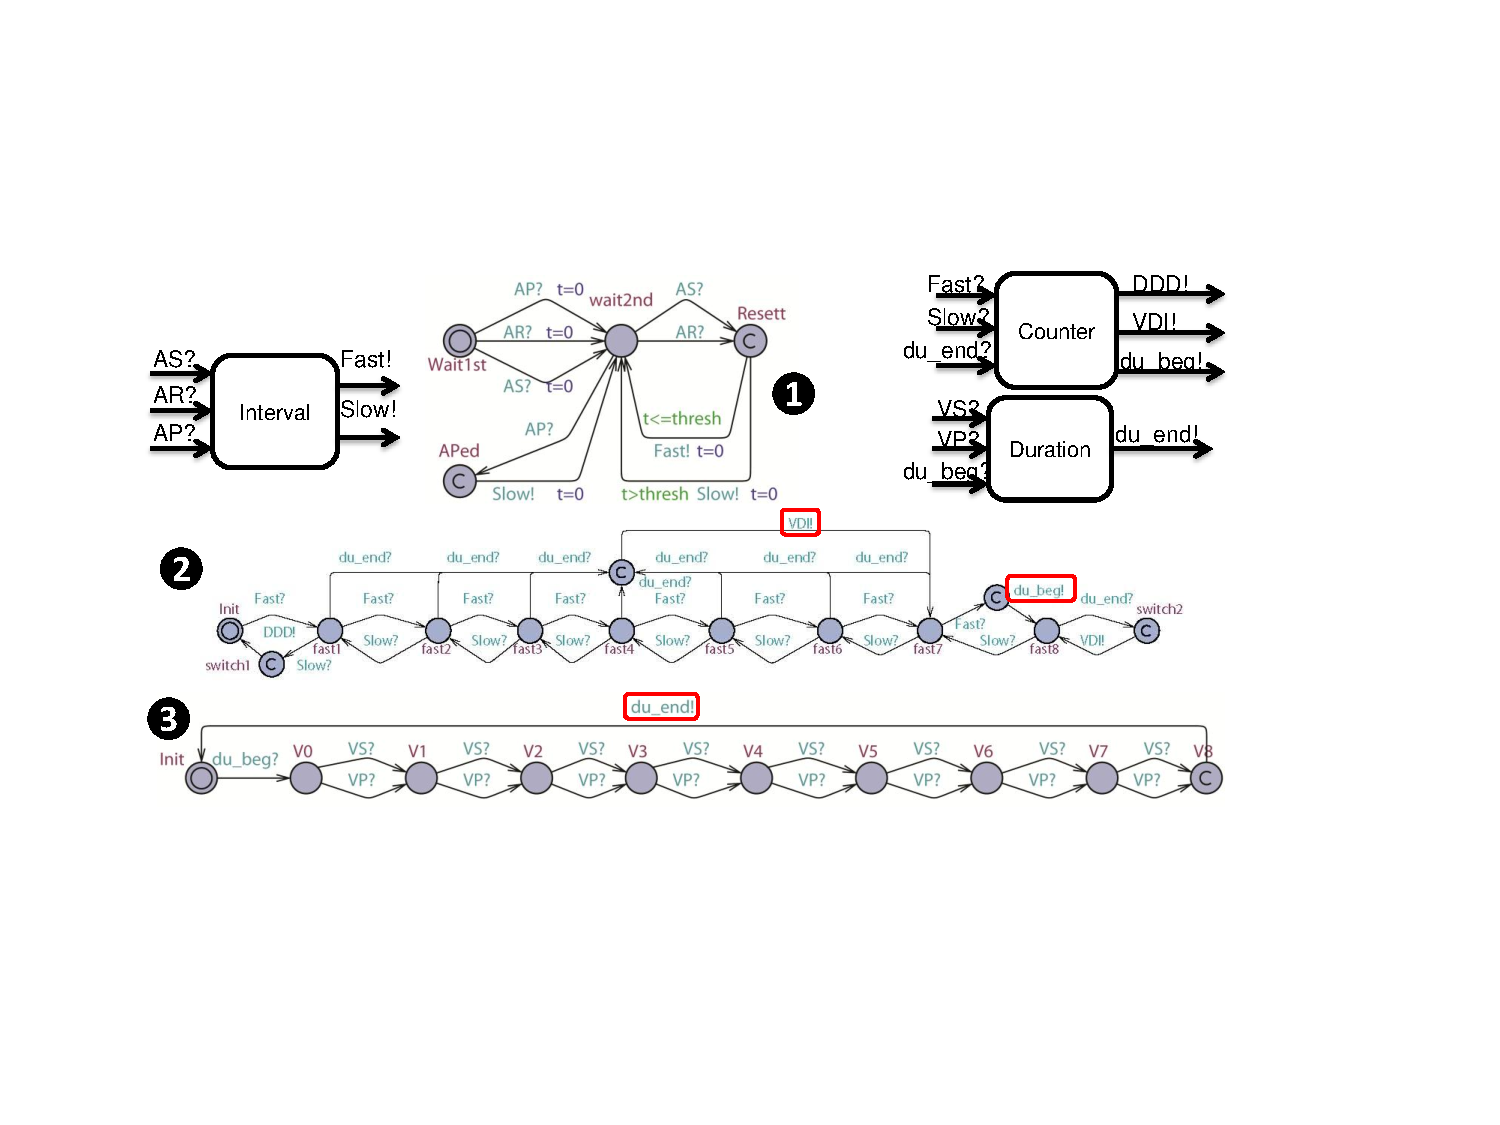
\includegraphics[width=0.9\textwidth]{figs/duration.pdf}
		\vspace{-10pt}
		\caption{\small (1) Component \textsf{INT}: An atrial event (\textsf{AS,AR}) arrives before \textsf{thresh} after the previous atrial event is regarded as a \textsf{fast} event. Atrial event arrives after \textsf{thresh} and \textsf{AP} are regarded as \textsf{slow} event; (2) Component \textsf{CNT}: After 8 \textsf{fast} event the algorithm will start a duration by sending \textsf{du\_beg} and will switch to \textsf{VDI} mode when the duration ends (\textsf{du\_end}); (3) Component \textsf{DUR} :The duration length is 8 ventricular events (\textsf{VS,VP})}
		  %\vspace{-15pt}
		\label{fig:dur_count}
\end{figure*} 

%%%%%%%%%%%%%%%%%%%%%%%%%%%%%%%%%%%%%%%%%%%%
%%%%%%%%%%%%%%%%%%%%%%%%%%%%%%%%%%%%%%%%%%%%

\chapter{Closed-loop Model Checking}
There are two categories of device bugs: 
1) the device may fail to conform to its \emph{specifications}, that is, the prescription of how it should react to certain inputs.  
2) the device may fail to improve the conditions of the patient as promised, even if it conforms to its specifications. 
The desired physiological conditions that the closed-loop system should achieve are captured in the \emph{physiological requirements}; for example, for a pacemaker, the heart rate should always be maintained above a certain threshold. 

Bugs in the first category (non-conformance to specification) can be detected via systematic and extensive open-loop testing in which a set of input sequences is fed to the device, and its output is compared with the expected output.
Bugs in the second category (violation of physiological requirements), on the other hand, require the interaction within the \emph{closed-loop system}, which consists of the device and its environment.
For instance, the pacemaker and the heart as its environment. 
In the medical device industry, closed-loop verification of the physiological requirements is mostly performed in terms of clinical trials, in which the actual devices are implanted in human subjects over an extended duration.
Unfortunately, because of the extremely high cost of clinical trials (several million dollars and spanning several years,~\cite{trialcost}), the amount and variety of human subjects during the clinical trials are limited, which reduces the opportunity to find bugs. 
Moreover, clinical trials are often conducted at the final design stage. Fixing bugs at this stage is very costly.

Closed-loop model checking enables closed-loop evaluation of the physiological requirements at an earlier design stage, which requires formal model(s) of the physiological environment. In this chapter we will answer the following questions:
\begin{itemize}
	\vspace{-5pt}
	\item How can we model environmental conditions of the heart to capture all physiological requirements?
	\vspace{-5pt}
	\item Can model checking find violations that testing cannot find?
	\vspace{-5pt}
	\item When and how to refine the environment model?
        \vspace{-5pt}
        \item Exploring the whole state space sounds great. What are the limitations of model checking? 
\end{itemize}
%            \item What are the effects of adding new features to the software? Can they disrupt the safety properties that the previous device hold?

In closed-loop model checking, there is only one device model. 
However there can be a large number of environmental conditions which require different models to represent them. For instance, a heart with atrial flutter has an additional conduction pathway, causing fast atrial rate, that is not present in a healthy heart. The timing and structural differences of different heart conditions should be distinguished in corresponding heart models.
%\todo[inline]{should we give an example of a heart condition?}
A set of initial models of the environment can be constructed, but the set is inherently incomplete because of the large number of environment conditions and their combinations. 
As a result, performing model checking using every model in the set cannot ensure full coverage of the environmental conditions. In the following sections, we will investigate how as we go from basic to more complex requirements, we require more sophisticated approaches to generate and navigate through a variety of environment models. We introduce the concept of an \emph{Abstraction Tree} to systematically encode requirements and choose the appropriate heart models for the requirement. By analyzing the concrete counter-examples we are able to distinguish if the problem is a bug within the device or due to the lack of expressivity in the environment model. 

\section{Testing vs Verification}

\newcommand{\ub}{\bar{u}}
\newcommand{\yb}{\bar{y}}

\emph{\textbf{Testing}} is a method for checking that a system does indeed obey its specification. 
In testing, an algorithm will do the following:
\begin{itemize}
	\item Initialize the system to some initial state $x_0$ in $X_0$.
	E.g., for a pacemaker device, this would describe the initial values for the various refractory periods, among other things.
	\item Generate sequences of input strings $\bar{u}_k$ from some set $A$, in reaction to which the system will produce output strings $\bar{y}_k$,
	\item A \emph{monitor} logs the output strings and determines whether the pair $(\bar{u}_k,\bar{y}_k)$ satisfies the specification or not.	
\end{itemize}

Because the set of valid initial states $X_0$ and the set of valid input strings $A$ may be infinite (or simply too large), the test bench must decide on how to intelligently choose a \emph{finite} number of $(x_0,\ub)$.
They must be chosen such that if the system does not produce wrong behavior with these pairs, then it is unlikely to produce errors under the \emph{full} valid set of pairs, namely, $X_0 \times A$.
This is the main challenge of testing: how to sample an infinite or large set of behaviors such that it is representative (in the above sense) of the full set of behaviors that $S$ is capable of?
Another important issue in testing is for how long to test the system: i.e. what should be the length of the $k^{th}$ string $\ub_k$? 
E.g., if $\ub_k$ has length 1000, the bug might manifest itself on $y_1\ldots y_{1001}$, but not $y_1\ldots y_{1000}$.

Regardless of the testing algorithm, testing remains incomplete, in the sense that short of testing every possible behavior, bugs may lie hidden in the behavior that we did not witness.

\emph{\textbf{Verification}} refers to formal verification.
It is applicable to finite state systems\footnote{Some infinite-state systems can be formally verified after an abstraction process which essentially produces an equivalent system that has finitely many states.}, 
and requires formal semantics for the system's operation. 
Roughly, this means we must have a mathematical unambiguous definition of how the system produces its output.
A verification algorithm, or \emph{model checker}, will explore the \emph{entire finite state-space} of the system in a systematic manner. 
Intuitively, if the entire state-space has been explored in all possible ways, and no incorrect behavior has been displayed, then the system is correct. 
Thus, verification is inherently \emph{complete}: if the model checker determines that the system is correct (under the conditions $A$ and $X_0$), then we can rest assured that is indeed the case.
Unlike testing, there is no question of whether we missed (didn't run) an initial condition that can display a bug.
There is also no question of test duration.
However in practice, some bound on the duration of the verification must be placed to avoid excessively long runs. 
If the model checker can't determine correctness in that time bound, then the verification is inconclusive.

Verification is computationally expensive and usually more burdensome to setup, but comes with a guarantee on the answer. 
Testing is computationally cheaper and less burdensome to setup, but the guarantees it provides are significantly weaker.
Testing, on the other hand, may be the only option for some complex systems that are beyond the capacity of today's model checkers, or which do not possess formal semantics.

In this chapter we cover formal verification of the closed-loop system and address testing in the following chapter.

\section{Reachability of Unsafe Regions for Basic Pacemaker Function}
The basic function of a pacemaker is to increase heart rate when necessary. As the result, we not only want to verify that the heart rate has been increased accordingly, but also ensure the pacemaker does not increase the heart rate too much. Since these requirements should hold for all possible heart conditions, the most abstract heart model $e$ is selected from Fig. 	\ref{fig:HM_abs} as the environment model. The following two requirements specify the unsafe regions  (too fast and too slow) within the closed-loop state space.

\subsection{Lower Rate Limit}
\vspace{-10pt}
The most essential function for the pacemaker is to treat bradycardia by maintaining the ventricular rate above a certain threshold. We define the region where the ventricular rate is slow, as \textsf{unsafe}. The monitor \textsf{PLRI\_test} is designed to measure intervals between ventricular events and is shown in \figref{safety1}. For property \\
\textsf{$\varphi_{LRI}=$A[] (PLRI\_test.secV imply PLRI\_test.t$\leq$TLRI)}\\ we have $H_4\| P\| PLRI\_test\models\varphi_{LRI}$.

\begin{figure*}[t]
\centering
%\vspace{-10pt}
		\subfigure[Monitor \textsf{PLRI\_test}] {
				\includegraphics[width=0.5\textwidth]{figs/LRI_test.pdf}
				\label{fig:safety1}
		} 
		\subfigure[Monitor \textsf{PURI\_test}] {	
			\includegraphics[width=0.45\textwidth]{figs/uri_test.pdf}
			\label{fig:uri_test}
		}
		%\vspace{-10pt}
	\caption{(a) Monitor for LRL: Interval between two ventricular events should be less than TLRI, (b) Monitor for URL: Interval between a ventricular event and a VP should be longer than TURI}
\vspace{-10pt}
\end{figure*} 

\subsection{Upper Rate Limit}
\vspace{-10pt}
The pacemaker is not designed to treat tachycardia so it can only pace the heart to increase its rate and cannot slow it down. However, it is still important to guarantee it does not pace the ventricles beyond a maximum rate to ensure safe operations. To this effect, an Upper Rate Interval (URI) is specified such that the pacemaker can increase the ventricular rate up to this limit. 

\begin{figure}[b]
		\centering
		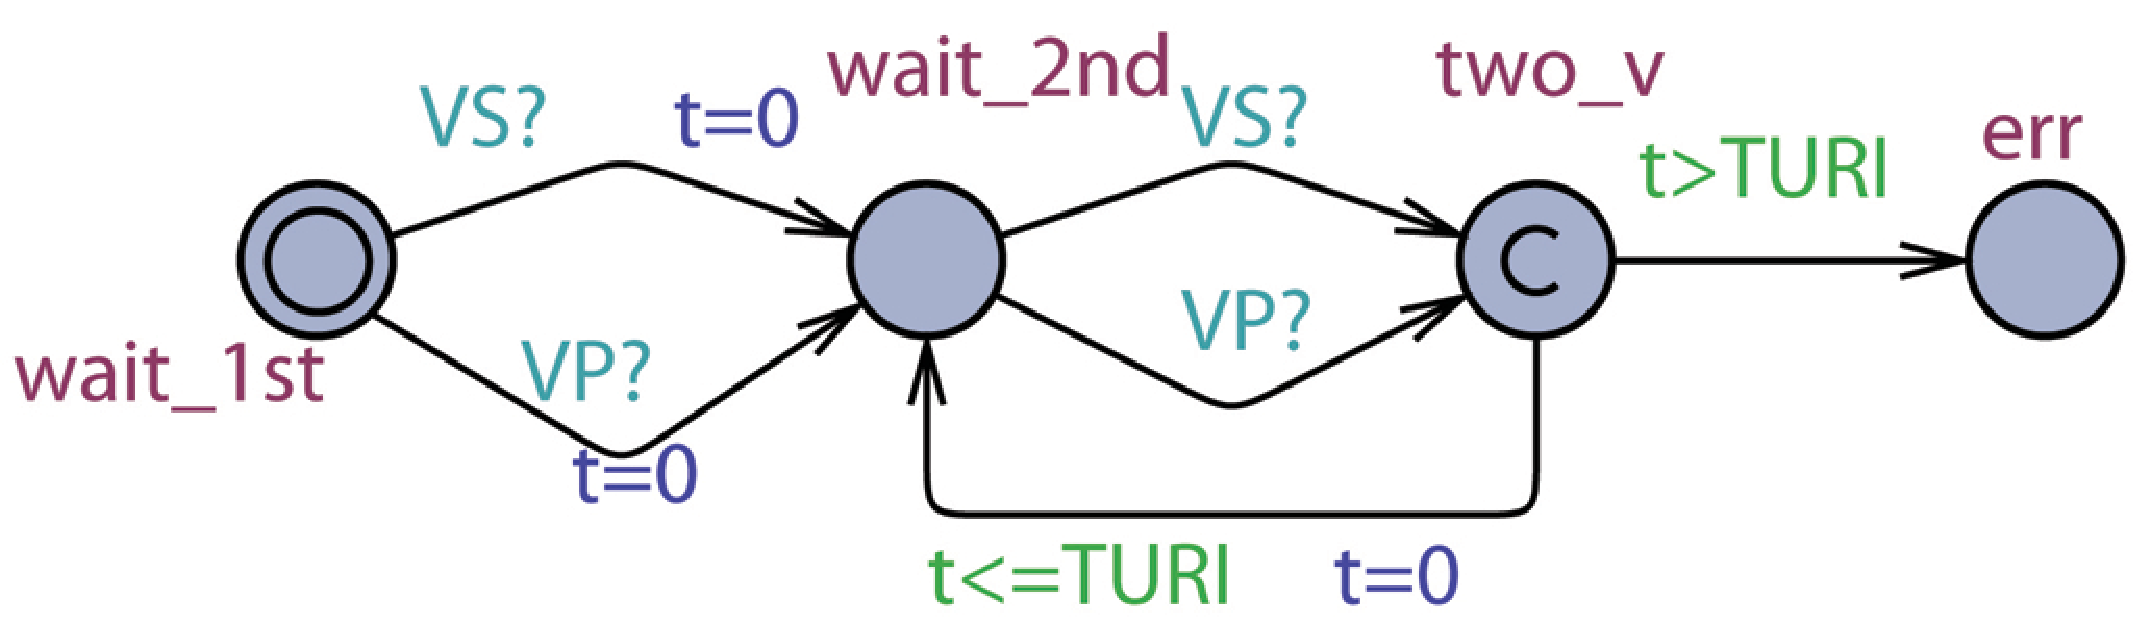
\includegraphics[width=0.4\textwidth]{figs/vv.pdf}
		\caption{\small Monitor \textsf{Pv\_v} for SVT: There exists an endless sequence in which interval between ventricular events is at most TURI}
		  %\vspace{-15pt}
		\label{fig:vv}
\end{figure}
  
We require that a ventricle pace (VP) can only occur at least $TURI$ after a ventricle event (VS, VP). The monitor \textsf{PURI\_test} is shown in \figref{uri_test}. For the property\\
$\varphi_{URI}=$\textsf{A[] (PURI\_test.secV imply PURI\_test.t$\geq$TURI)} \\
we have $H_4\| P\| PURI\_test\models \varphi_{URI}$.

\section{Model Checking the Mode-Switch Algorithm}

\subsection{Existence of Pacemaker Mediated Tachycardia during SVT}
The monitor \textsf{Pv\_v} is designed to show existence of PMT during SVT. It goes to the error state if the ventricular rate drops below the Upper Rate Limit (\figref{vv}).  


We specify 
$\varphi_{MS}=E[] (not Pv\_v.err)$\\
which verifies the existence of PMT. The heart model $H_e$ in Fig. \ref{fig:HM_abs} is not suitable for this property since the non-deterministic conduction of component $P_3$ does not capture the blocking property of the AV node, which is the key in PMT. We use a more refined model $H_d$ which has AV node modeled. To identify the PMT scenario, we first set $H_d.N^1.Trest\_min<100$ so that the atrial rate can be high and $H_d.N^2.Trest\_min>TURI$ so that the intrinsic heart rate is less than TURI. The property is first verified on pacemaker without the mode-switch algorithm. We have $H_d\|P\|Pv\_v\models\varphi_{MS}$ and the evidence returned by the model checker illustrates the PMT scenario.

% There are two separate AVI and LRI components for each mode and switches to the corresponding ones when synchronization signals are received. The clock values are kept so that essential intervals are kept. 
\subsection{Verification against fundamental safety properties}
For a pacemaker with the mode-switch algorithm: $P_2$=\textsf{LRI'$\|$AVI'$\|$URI$\|$PVARP$\|$VRP$\|$INT$\|$CNT$\|$DUR}, we verify the same fundamental safety properties on the pacemaker model with mode-switch algorithm. We have:
$$H_d\|P_2\|PURI\_test\models\varphi_{URI}$$
$$H_d\|P_2\|PLRI\_test\not\models\varphi_{LRI}$$
The Upper Rate Limit property still holds, but the Lower Rate Limit property is violated. The counterexample is proved to be valid after checking the trace of more refined heart models. By analyzing the trace we found that when the pacemaker is switching from VDI mode to DDD mode, the responsibility to deliver VP switched from LRI component to AVI component. Since the clock reference is different (Ventricular events in LRI component and Atrial events in AVI component), the clock value for delivering the next VP is not preserved. As a result, if an atrial event which triggered the mode-switch from VDI to DDD happens within [TLRI-TAVI, TLRI) after the last ventricular event, the next ventricular pacing will be delayed by at most TAVI time, which violates the Lower Rate Limit property (\figref{safety}). 
%%\begin{figure}
%%		\centering
%%		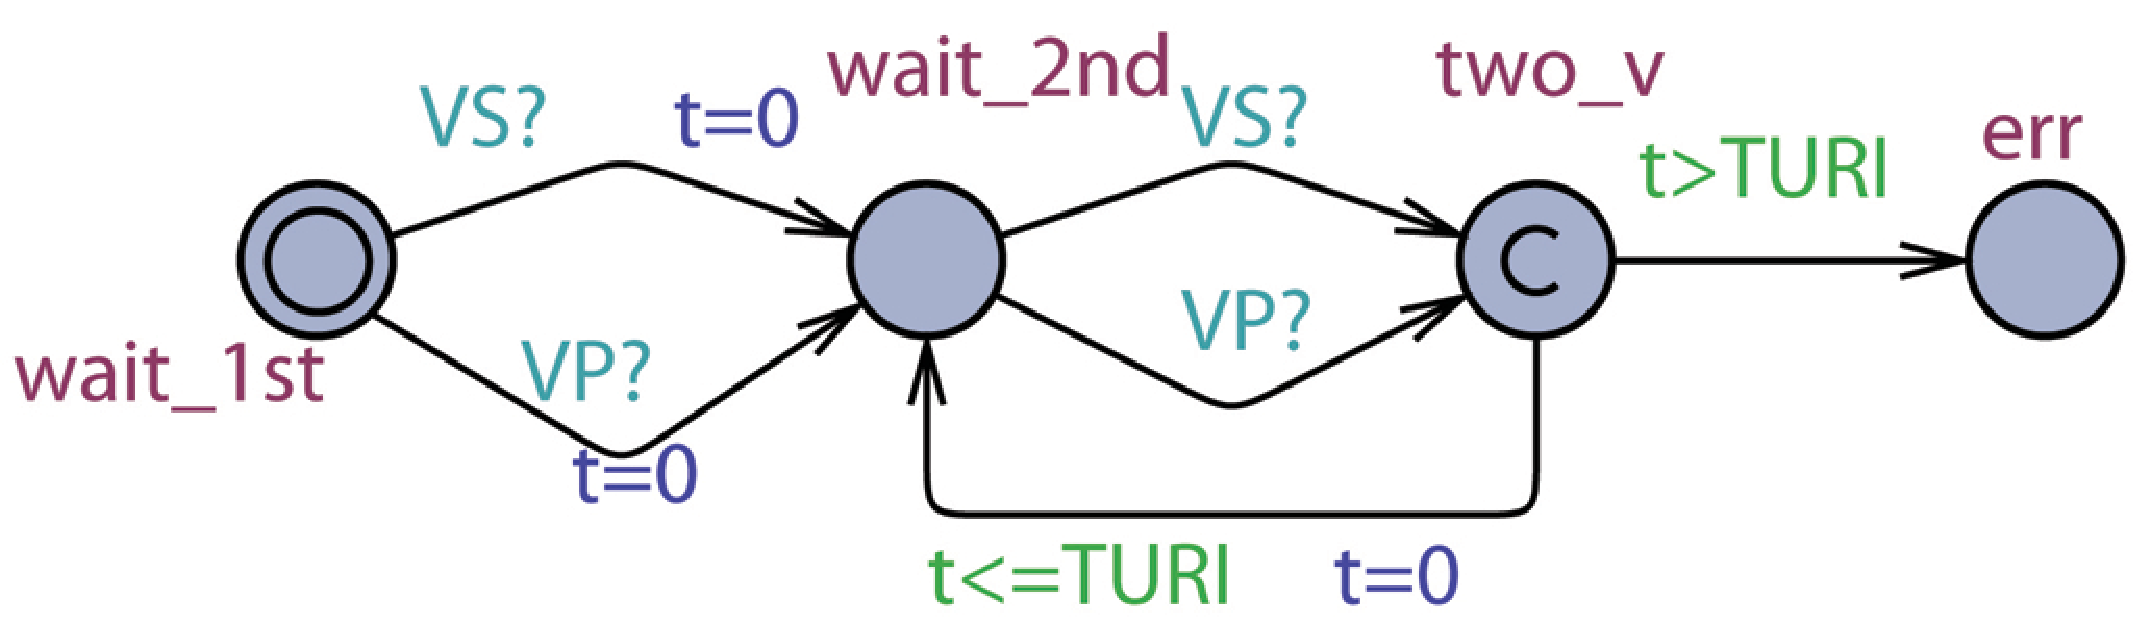
\includegraphics[width=0.4\textwidth]{figs/vv.pdf}
%%		\caption{\small Monitor \textsf{Pv\_v} for SVT: There exists an endless sequence in which interval between ventricular events is at most TURI}
%%		  %\vspace{-15pt}
%%		\label{fig:vv}
%%\end{figure}
\subsection{Verification of the Mode-Switch Algorithm}
After implementing the mode-switch algorithm, we verified the model against the same existence property. We expect the violation of this property, since during VDI mode the ventricular rate of the heart model is less than the Upper Rate Limit and will not trigger ventricular pacing. However, this property is still satisfied, indicating the mode-switch algorithm failed to eliminate the PMT scenario. The evidence trace returned by UPPAAL shows that a subset of atrial events fall into the blanking period after a ventricular event (see \figref{liveness}). As a result, two fast events are reduced to one slow event and mode switch may never happen. This scenario does exist in all our refined heart models, we conclude that the trace is physiologically feasible. The mode-switch algorithm in our pacemaker model can not terminate all PMT behaviors as specified.
\begin{figure}
\centering
%\vspace{-20pt}
		\subfigure []{
				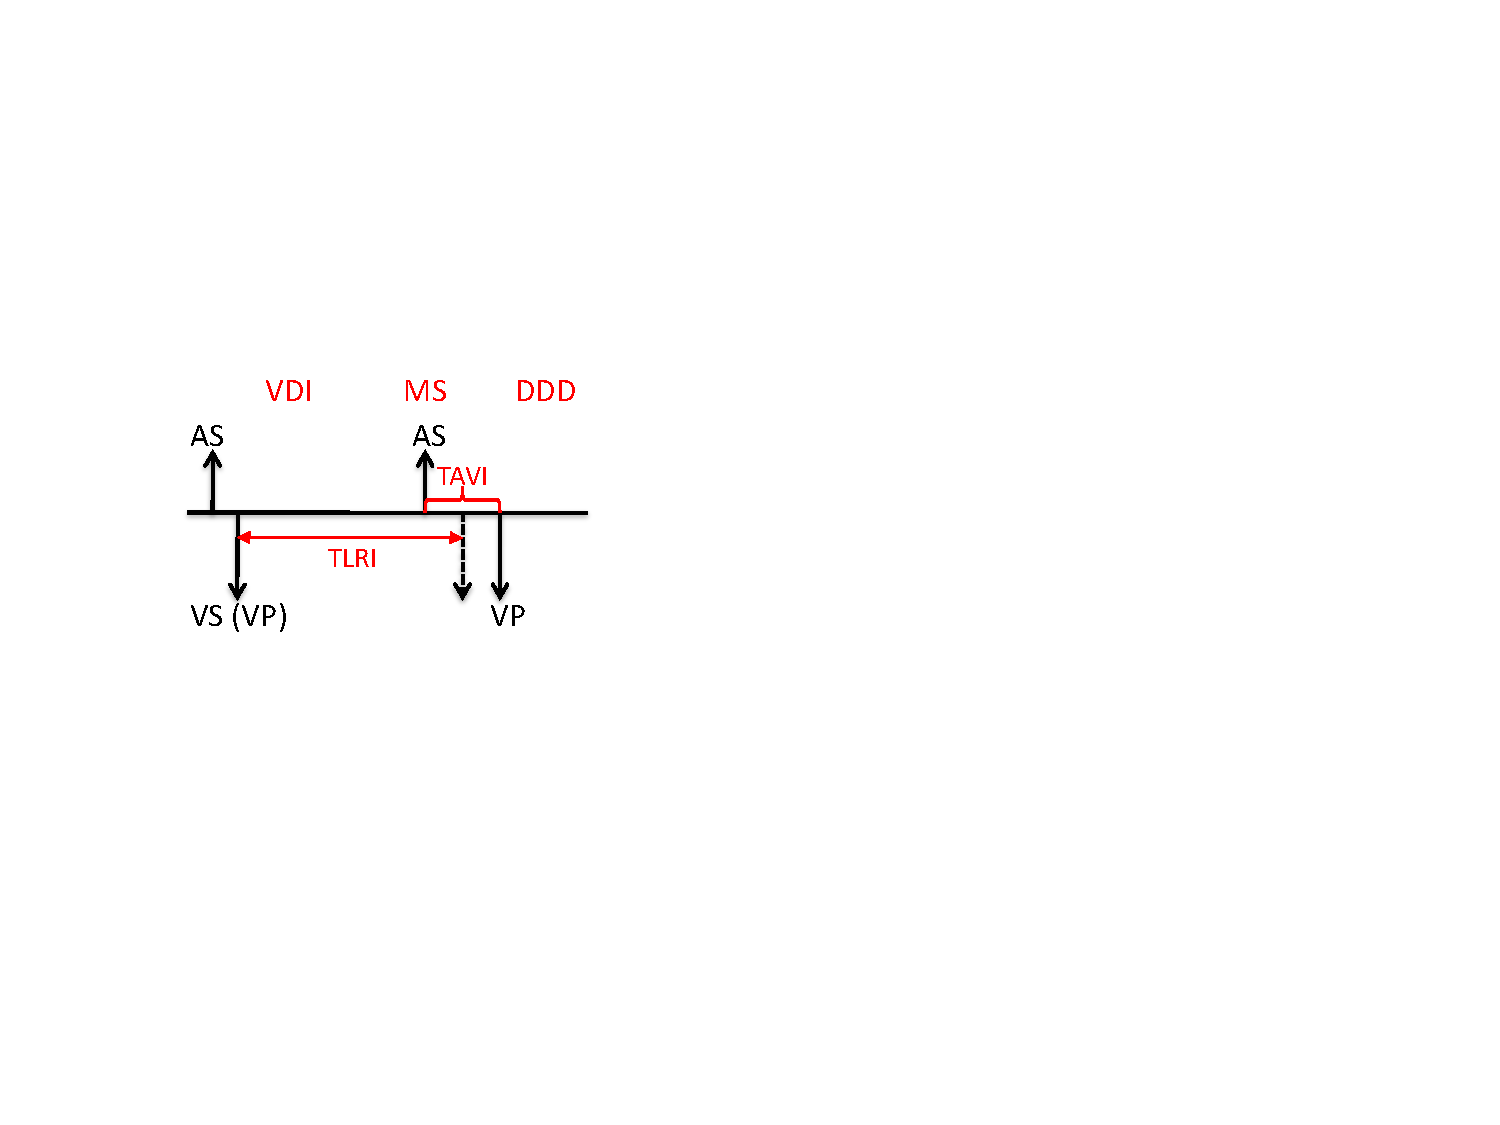
\includegraphics[width=0.4\textwidth]{figs/safety.pdf}
				\label{fig:safety}
		} 
		\subfigure []{	
			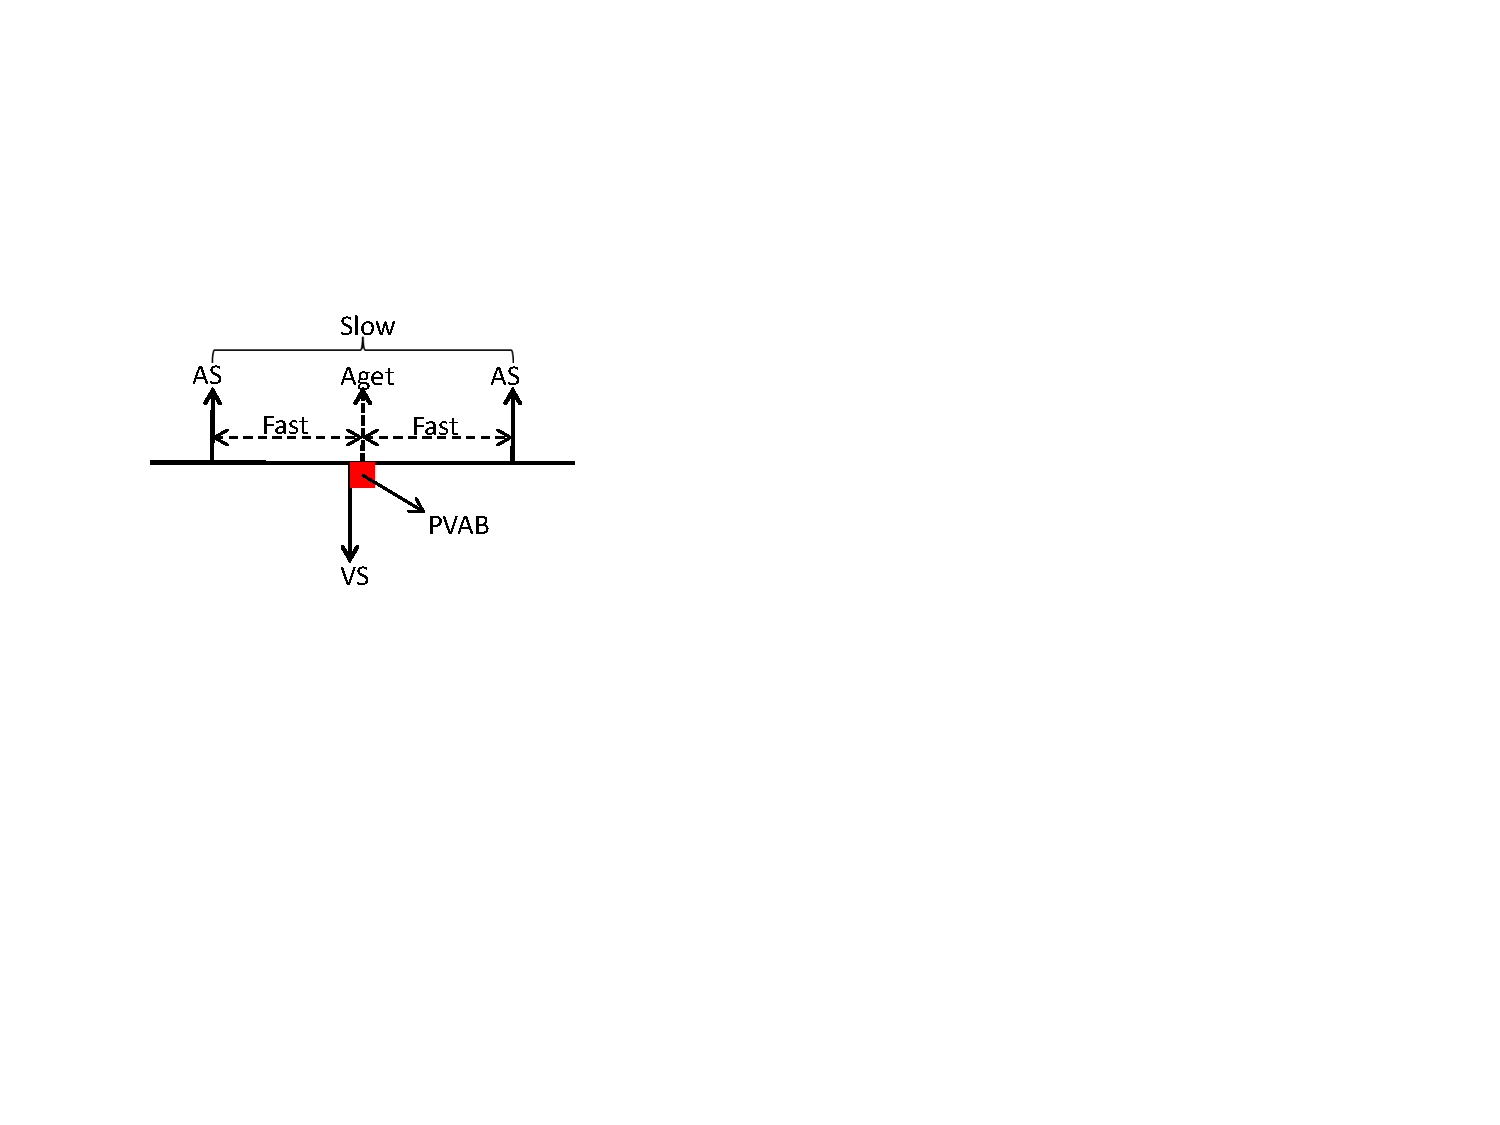
\includegraphics[width=0.4\textwidth]{figs/liveness.pdf}
			\label{fig:liveness}
		}
		\vspace{-10pt}
	\caption{(a) Safety Violation: VP is delayed due to the reset of timer during mode-switch, (b) Correctness Violation: The blocking period may block some atrial events, turning two \emph{Fast} events to one \emph{Slow} event \cite{TACAS12}}
\vspace{-20pt}
\end{figure} 
\section{Abstraction Tree for Environment Modeling}
In the previous two sections, model abstractions and selections are perfomed manually, which require knowledge of both Electrophysiology and model checking. 
Counter-examples returned from abstract models can be difficult to interpret by domain experts.
One abstract counter-example could be produced by multiple physiologically valid conditions, which causes ambiguity.
Thus, a rigorous framework is necessary to balance the need to cover a wide range of environmental conditions and the need to provide counter-examples to the physicians within their physiological context. The framework must also allow non-domain experts to perform verification, and establish `hand-off' points where the results of verification can be handed back 
to the experts for interpretation.

In this section, we use a set of domain-specific abstraction rules developed based on physiological knowledge to ensure the physiological relevance of the behaviors introduced into the abstract models.
The rules are applied to an initial set of physiological models to obtain an abstraction tree, which will be used for closed-loop model checking of the pacemaker. 
A straightforward search procedure is then used to conduct model checking using suitable heart models and return the most concrete and unambiguous counter-examples to the physicians for analysis.
In this framework, physiological knowledge is only needed when constructing the initial model set and when analyzing counter-examples. 
The application of the physiological abstraction rules and the verification procedure can be automated.
The proposed method can potentially be generalized to other domains in which the device operates in a large variety of environmental conditions. More information regarding this research can be found in \cite{regar_tech}.
\subsection*{Step 1: Abstraction Tree Construction}
A set of heart models corresponding to different heart conditions are first developed. 
The list can be expanded as new heart conditions are discovered.
Because we start from a set of initial models, and each one may be abstracted using a number of abstraction rules, we have a choice of which rules to apply to which models, and the order in which to apply them. 
Depending on which rule is applied when, we end up with different abstract models.
Thus an \emph{abstraction tree} $T_{HM}$ for the heart is created, as shown in \figref{HM_tree}. 
%Note that applying rules in different order results different abstraction tree. 
%The order used to obtain $HM\_tree$ is based on the domain knowledge that certain heart conditions may have similar behaviors and similar inputs to the pacemaker. 
%This systematic grouping maintains the physiological-relevance of the heart model even at higher abstraction levels, and reduce the necessity to resolve ambiguities at lower abstraction levels when model checking certain requirements.
\begin{figure}[!t]
	\centering
	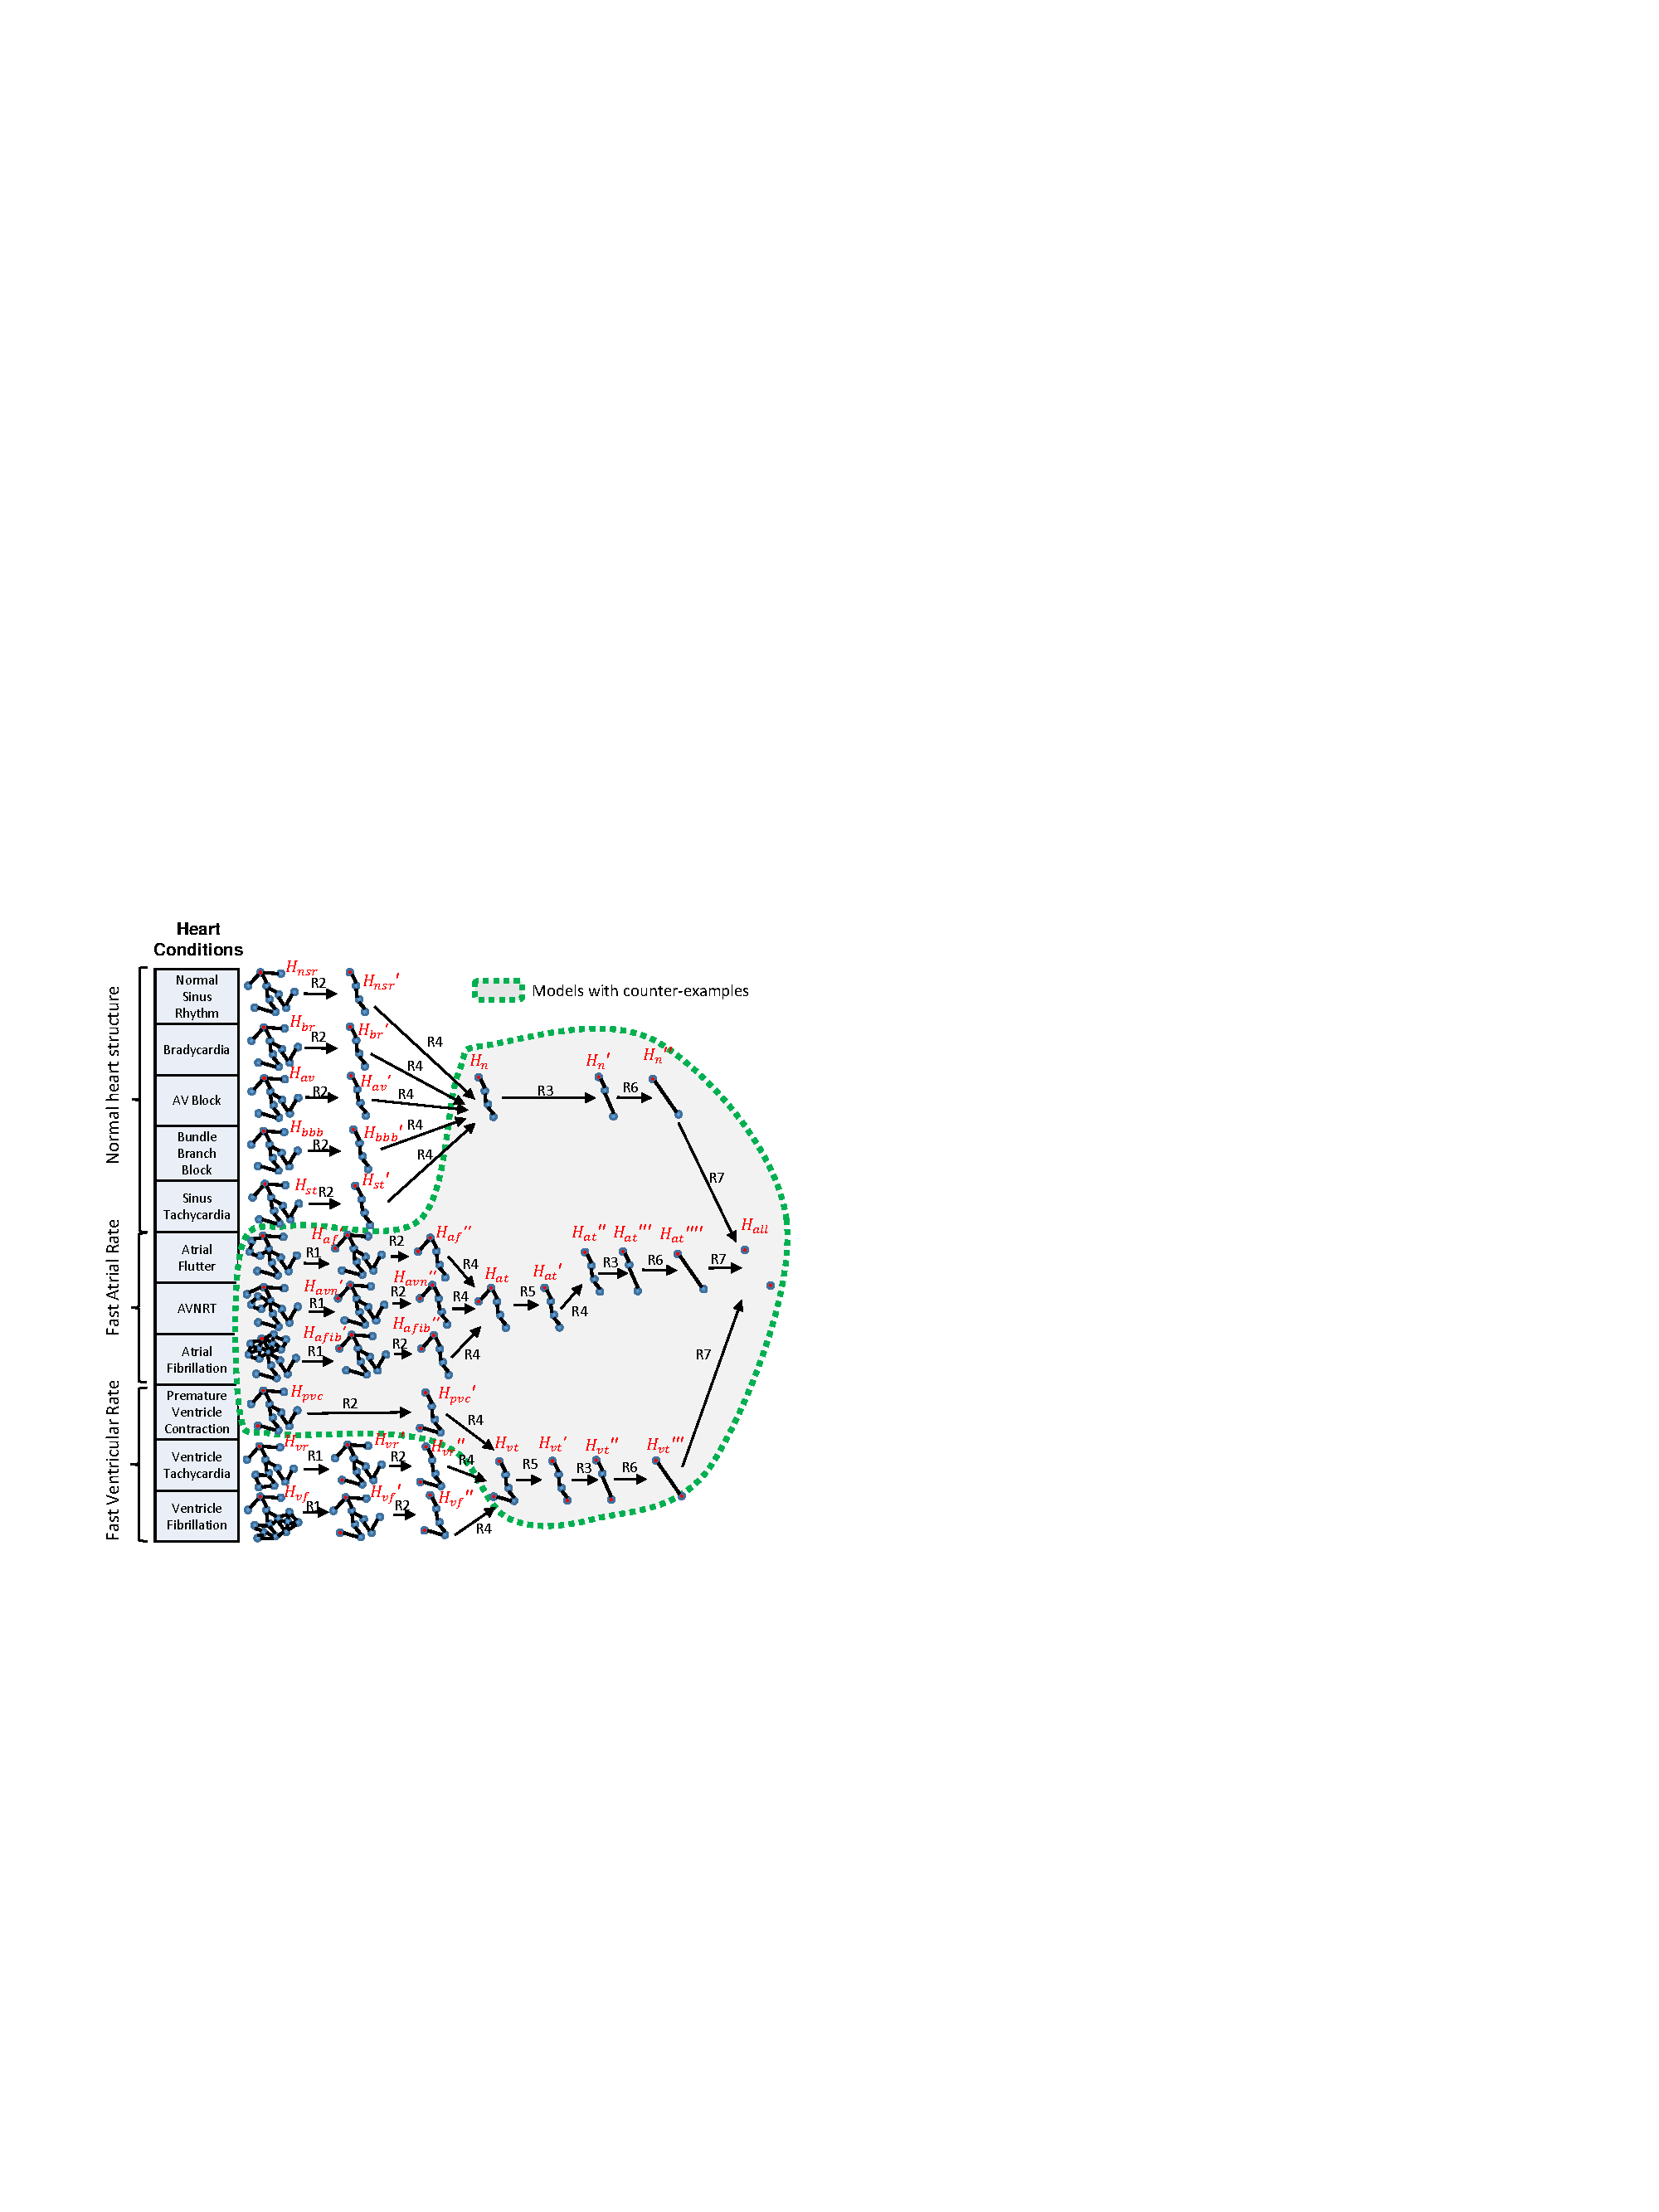
\includegraphics[width=0.85\textwidth]{figs/abs.pdf}
	%\vspace{-5pt}
	\caption{\small Heart Model Abstraction Tree}
	\vspace{-15pt}
	\label{fig:HM_tree}
\end{figure}

\subsection*{Step 2: Requirement Encoding}
The following requirement is designed to prevent the pacemaker from pacing too fast: 
``If the intervals between self-activations of the atria are between 300ms to 1000ms (60bpm - 200bpm), the intervals between ventricular paces should be no shorter than 500ms.''
Self-activation of the atria can be expressed using the location and clock of node automaton $N_A$.
The requirement can be formalized using the monitor  $M_{sing}(VP,500,\infty)$:
%\hatodo{mention $N_A$ is the atrium node automaton}
\[Req1: N_A.loc=Rest \land N_A.t\in [300,1000] \Rightarrow \neg M_{sing}.loc==Err\]
%\todo[inline]{some figure captions are all caps, others are not. please use same thing throughout}
%\begin{figure}[!b]
	%\centering
	%\vspace{-10pt}
	%\includegraphics[width=0.5\textwidth]{figs/abs_sim.pdf}
%
	%\caption{\small Abstraction Rule Application Example}
%\vspace{-10pt}
	%\label{fig:abs_exam}
%\end{figure}
 \subsection*{Step 3: Choosing Appropriate Heart Models For the Requirement}
To verify the closed-loop system with pacemaker model $PM$ and abstraction tree $T_{HM}$ (\figref{HM_tree}) against requirement $Req1$, the most abstract appropriate models are selected from the tree. 
The single event monitor $M_{sing}$ from \figref{monitor}(a) with variables $Var(M_{sing})=\{M_{sing}.t,M_{sing}.loc\}$ is used for this requirement. Model checking is performed on the closed-loop system including the heart model $M_H$, the pacemaker model $M_P$, and the monitor $M$. The requirement $\varphi_P$ can be then represented with TCTL formula:
 \textsf{A[] (not M.Err)}

The variables in the requirement are:
$Var(Req1)=\{N_A.t,N_A.loc,M_{sing}.loc\}$.
\begin{figure}[b]
		\centering
		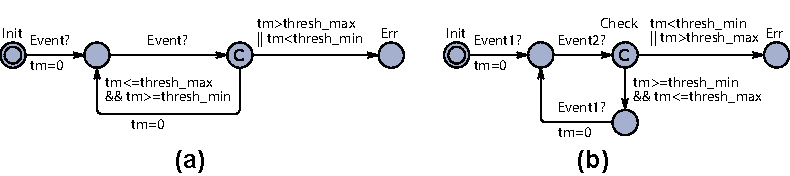
\includegraphics[width=0.8\textwidth]{figs/monitor.pdf}
		%\vspace{-5pt}
		\caption{\small (a) $M_{sing}$ for single event; (b) $M_{doub}$ for two events}
		  \vspace{-10pt}
		\label{fig:monitor}
\end{figure}

At the root of the tree $H_{all}$, we have $\{N_A.t,N_A.loc\} \not \subset Var(H_{all})\cup Var(M_{sing})$. 
So $H_{all}$ is not appropriate for $Req1$. 
All the children of $H_{all}$: $H_n'',H_{at}'''',H_{vt}'''$ are appropriate for $Req1$,
%we have $Var(Req1)\cup Var(M_{sing})\subset Var(H_n'')=Var(H_{at}'''')=Var(H_{vt}''')$, 
thus these three heart models are output as the most abstract models that are appropriate for $Req1$.
\begin{figure}[!t]
	\centering
	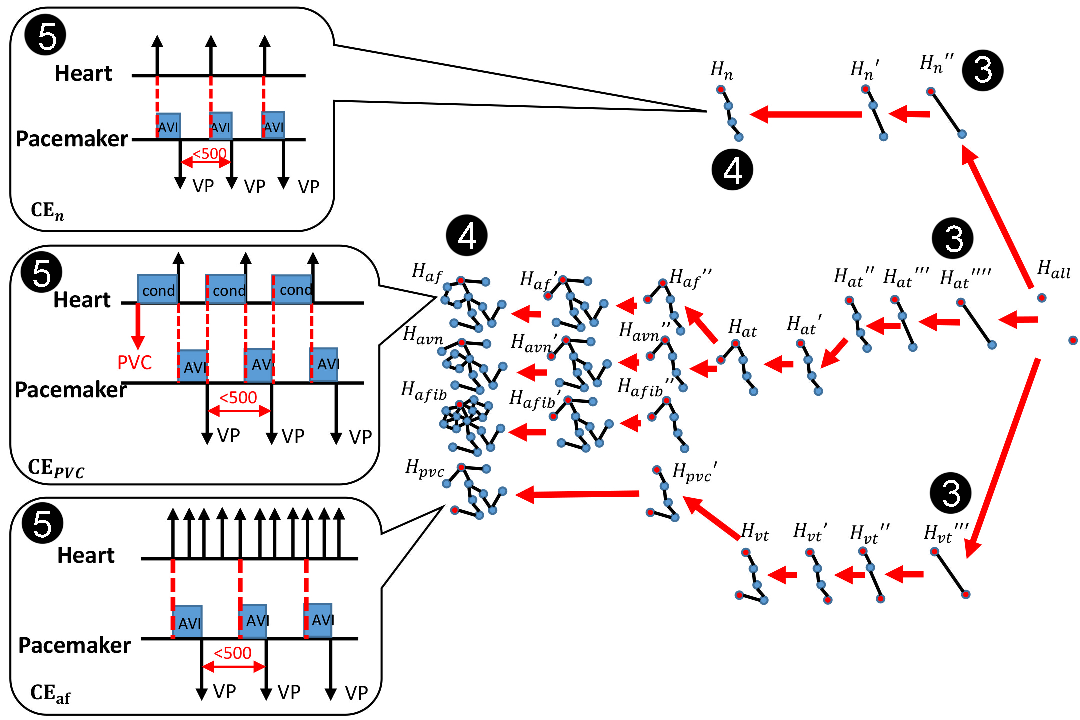
\includegraphics[width=0.8\textwidth]{figs/abs_rev.pdf}
	%\vspace{-5pt}
	\caption{\small Finding the most concrete counter-examples using the abstraction tree}
	\vspace{-10pt}
	\label{fig:CE}
\end{figure}
	\vspace{-10pt}
\subsection*{Step 4: Return the most Concrete Counter-Examples}
After the appropriate models for $Req1$ are selected, we have the initial set
$HM=\{H_n'',H_{at}'''',H_{vt}'''\}$.
Then we run Algorithm 2. By model checking on all 3 initial models in UPPAAL we have: 
$$H_n''||PM\not\models Req1;\; H_{at}''''||PM\not\models Req1;\; H_{vt}'''||PM\not\models Req1$$
%$$[1,[]]=ModelChecking(H_n'',PM,Req1)$$
 %$$[0,CE_1]=ModelChecking(H_{at}'''',PM,Req1)$$
%$$[0,CE_2]=ModelChecking(H_{vt}''',PM,Req1)$$
%\hatodoin{In the following text you use $CE_{at}$, etc. It's  best to use the letter subscripts in the above equations as well, so it's clear which cex comes from which heart model.}
%For the two heart models $H_{at}'''',H_{vt}'''$ in which the requirement is violated, the algorithm keeps going down the abstraction tree, and upon termination counter-examples are returned for the following heart models
The abstraction tree is then further explored. The heart models with counter-examples are illustrated in \figref{CE}, and the most refined heart models with counter-examples are: $H_{n};H_{pvc};H_{af};H_{avn};H_{afib}$.
%$$[0,CE_{at}]=ModelChecking(H_{at},PM,Req1)$$
%$$[0,CE_{pvc}]=ModelChecking(H_{pvc},PM,Req1)$$
%$$[0,CE_{af}]=ModelChecking(H_{af},PM,Req1)$$
%$$[0,CE_{avn}]=ModelChecking(H_{avn},PM,Req1)$$
%$$[0,CE_{afib}]=ModelChecking(H_{afib},PM,Req1)$$

%\begin{figure}[!t]
		%\centering
		%\includegraphics[width=0.9\textwidth]{figs/case.pdf}
		%%\vspace{-5pt}
		%\caption{\small Counter-examples}
		  %\vspace{-10pt}
		%\label{fig:CE}
%\end{figure}
	\vspace{-10pt}
\subsection*{Step 5: Analysis of the Counter-examples}
The counter-examples are then shared with physicians for analysis. In \figref{CE} we highlight three counter-examples. In the first counter-example, the intrinsic heart signals over time with up arrows as atrial activations and down arrows as ventricular activations. The signal for the second counter-example shows the pacemaker outputs with up arrows as atrial pacing and down arrows as ventricular pacing.%We only show the activations of the atrial node and ventricle pacing. 

Counter-example $CE_{n}$ is returned by $H_n$ and none of its children models violate the requirement. By careful analysis we found that $CE_{n}$ features the combination of fast intrinsic atrial rate and prolonged A-V conduction delay, which is the combination of heart conditions $H_{st}$ and $H_{av}$. This scenario shows that the abstraction rules can introduce physiological heart conditions that were not explicitly modeled in the initial model set. The pacemaker improved the open-loop heart condition by pacing the ventricles $AVI$ after each atrial event, which is a correct operation of the pacemaker despite the requirement violation. 
%\hatodo{is it TAVI or AVI like in the previous seciton?}

%\hatodoin{Do you mean that $CE_{at}$ is not a bug? Does this mean that the requirement may be violated in ways that are not dangerous?}
Counter-example $CE_{pvc}$ has a very similar execution to $CE_{n}$. However, the activations of the atrial node are triggered by retrograde conduction from ventricular paces (marker \textsf{cond}). The atrial activations trigger another ventricular pace after $AVI$, which will trigger another retrograde conduction. In this case, the heart rate is inappropriately high, which corresponds to a dangerous closed-loop behavior referred to as \emph{Endless Loop Tachycardia}.

In counter-example $CE_{af}$, the atrial rate is very high, which is also a sub-optimal but not dangerous heart condition. 
However, the ventricular rate can stay normal due to the blocking property of the AV node. 
Despite the filters in the pacemaker, the pacemaker still paces the ventricle for every 3 atrial activations, which extends fast atrial rate to more dangerous fast ventricular rate. 
%\hatodoin{Not very clear..do you mean that the intrinsoc centricular rate is fine because of AV filtering, but the PM is accelarating it?}
This scenario is referred to as Atrial Tachycardia Response of a pacemaker. 

From the analysis, pacemaker operations in $CE_{pvc}$ and $CE_{af}$ must be revised. However, the revision should not affect the behavior in $CE_{n}$. This example demonstrates that counter-examples from refined models provide more physiological context of the requirement violations, and distinguish the physiological conditions that can trigger the violations. The information is helpful for debugging and improving the algorithm. The physicians can also improve the physiological requirement so that these heart conditions can be then considered case by case.




\chapter{Certification}
\begin{itemize}
          	\item Can model-based closed-loop verification provide more safety guarantee than current practice? How much?
          \end{itemize}
\section{Current Practice}
There are two mechanisms that a medical device can enter the market in U.S. The Premarket Notification, also known as 510(k), is the most common and simple way. In a 510(k) submission The general philosophy for FDA certification is the "`Least Burden Approach"'
\section{Model-based Proof of Confidence}
%\cite{pancreas}



\backmatter





\bibliographystyle{plainnat}
\bibliography{bibliography}

\end{document}